\documentclass[article,type=msc,colorback,accentcolor=tud2d,twoside]{tudthesis}
\usepackage{ngerman}
\usepackage[american,ngerman]{babel}
\usepackage{tabularx} % better tables
\usepackage{colortbl}
\usepackage[hyphens]{url}
\usepackage[ngerman]{hyperref}	% urls
\usepackage{enumitem}
\usepackage{color}
\usepackage{listings}	% nicer lists
%setup special characters in listing
\lstset{literate=
  {á}{{\'a}}1 {é}{{\'e}}1 {í}{{\'i}}1 {ó}{{\'o}}1 {ú}{{\'u}}1 {ù}{{\`u}}1
  {Á}{{\'A}}1 {É}{{\'E}}1 {Í}{{\'I}}1 {Ó}{{\'O}}1 {Ú}{{\'U}}1
  {à}{{\`a}}1 {è}{{\'e}}1 {ì}{{\`i}}1 {ò}{{\`o}}1 {ò}{{\`o}}1
  {À}{{\`A}}1 {È}{{\'E}}1 {Ì}{{\`I}}1 {Ò}{{\`O}}1 {Ò}{{\`O}}1
  {ä}{{\"a}}1 {ë}{{\"e}}1 {ï}{{\"i}}1 {ö}{{\"o}}1 {ü}{{\"u}}1
  {Ä}{{\"A}}1 {Ë}{{\"E}}1 {Ï}{{\"I}}1 {Ö}{{\"O}}1 {Ü}{{\"U}}1
  {â}{{\^a}}1 {ê}{{\^e}}1 {î}{{\^i}}1 {ô}{{\^o}}1 {û}{{\^u}}1
  {Â}{{\^A}}1 {Ê}{{\^E}}1 {Î}{{\^I}}1 {Ô}{{\^O}}1 {Û}{{\^U}}1
  {œ}{{\oe}}1 {Œ}{{\OE}}1 {æ}{{\ae}}1 {Æ}{{\AE}}1 {ß}{{\ss}}1
  {ç}{{\c c}}1 {Ç}{{\c C}}1 {ø}{{\o}}1 {å}{{\r a}}1 {Å}{{\r A}}1
  {€}{{\EUR}}1 {£}{{\pounds}}1
}
\lstset{breaklines=true}
\lstset{numbers=left}
\lstset{tabsize=2}
\usepackage{cleveref}
\usepackage{lineno}
\usepackage{colortbl}
\usepackage{longtable}
\usepackage{subfigure}
\usepackage{pdfpages}
\usepackage{titlesec}
\lstset{numbers=none}
\usepackage{amsmath}
\newcommand{\sectionbreak}{\clearpage}

\addto\extrasamerican{%  
  \def\subfigureautorefname{\figureautorefname}
  \def\subsectionautorefname{\sectionautorefname}
  \def\subsubsectionautorefname{\sectionautorefname}
  \def\subsubsubsectionautorefname{\sectionautorefname}
}




\graphicspath{{graphix/}}

\newcounter{dummy} % necessary for correct hyperlinks (to index, bib, etc.)

\linespread{1.2}\selectfont

\newcommand{\getmydate}{%
  \ifcase\month%
    \or Januar\or Februar\or M\"arz%
    \or April\or Mai\or Juni\or Juli%
    \or August\or September\or Oktober%
    \or November\or Dezember%
  \fi\ \number\year%
}

%\definecolor{rowColorHead}{rgb}{0.7,0.7,0.7}
%\definecolor{rowColor1}{rgb}{0.9,0.9,0.9}
%\definecolor{rowColor2}{rgb}{255,255,255}

\hypersetup{%
  pdftitle={Design, implementation and evaluation of an anti-phishing app},
  pdfauthor={Clemens Bergmann und Gamze Canova},
  pdfview=FitH,
  pdfstartview=FitV
}

\setinstitutionlogo[height]{graphix/secuso.jpg}

\begin{document}
\selectlanguage{american}
\pagenumbering{arabic}
  \thesistitle{Design, Implementation and Evaluation of an Anti-Phishing Education App}{Design, Implementierung und Evaluation einer Anti-Phishing Education App}
  \author{Clemens Bergmann und Gamze Canova}
  %\birthplace{Darmstadt}
  \referee{Professor Dr. Melanie Volkamer}{Arne Renkema-Padmos}
  \department{Fachbereich Informatik}
  \group{Security, Usability and Society}
  \tuprints{37639}{id/eprint/3763}
  \makethesistitle
  \affidavit{C. Bergmann}
  \affidavit{G. Canova}
\cleardoublepage
 \tableofcontents

	%======================================================
	% CONTENT
	%======================================================
	\cleardoublepage
		
	% !!!!!!!!!!! WOERTER VEREINHEITLICHEN: !!!!!!!!!!!
	%anti-phishing
	%capitalization
	%email / e-mail / mail
	%website / web site
	%... e.g. und for example.
	% Therefore, ... (KOMMA)
	% Also, .... (KOMMA)
	% Additionally etc....
	% pre-study/prestudy mit phishing survey ersetzen!!!
	% can not / cannot
	% address bar / URL-bar / URL bar
	%	\linenumbers

	%Abstract:
	\begin{abstract}	
Scammers discover the Internet as a convenient place for their criminal activities. 
For instance, they send Internet users spoofed e-mails or publish fraudulent websites which prompt users to enter their confidential data. 
This kind of Internet fraud is referred to as phishing. 
For a victim of a phishing attack the consequences can be of an economic as well as an emotional nature. 
There exist multiple technical solutions to approach the problem of phishing. 
Yet, they all cannot guarantee 100\% accuracy.
Moreover, sometimes security warnings or indicators of such approaches are ignored by end-users.
For this reason a complementary approach is required.
We believe that the increase of security awareness and especially user education about the dangers of the Internet, is a further key strategy to combat phishing. 
Our master thesis aims at developing a smartphone app, which increases security awareness and educates the user regarding phishing.
To increase security awareness the users send themselves a spoofed e-mail right away when starting the app for the first time.
This shall exemplary illustrate them how trivial e-mail spoofing is and is intended to increase their motivation and engagement ultimately leading to better knowledge retention.
The user education part entails alerts regarding known techniques of attackers and helps them to internalize these by practice and repetition.
In detail, our app is realized as a quiz based game which mainly focuses on the detection of phishing URLs.
Ultimately, the app should enable the users to achieve the capability of defending themselves against phishing attacks in the future, in case technical solutions should fail.
In order to evaluate the effectiveness of the app a user study is conducted.
The study outcomes shows that our app in general receives positive feedback from the users and also helps them make better decisions on whether a given URL is legitimate or fraudulent.
\end{abstract}
	%*******************************************
%*******************************************
\section{Introduction}
%*******************************************
\label{s:introduction}

Nowadays, a world without Internet is unimaginable for most people in developed countries.
As an example, 83\% of Germany's population has Internet access~\cite{globalfinance2012internetusage}. 
However, it is undeniable that with the benefits of the Internet also come threats. 
One major issue of today's digitalized world is phishing. 
Phishing is a term which is referred to for various scenarios and techniques resulting in multiple possible definitions.
\autoref{s:phishing_general} elaborates on the different phishing techniques and scenarios.
Within the scope of this work, however, phishing is a form of fraud which lures users into disclosing confidential information. 
Usually, phishing happens through fake websites which imitate the original ones.
On these fraudulent website the users are persuaded to enter their confidential data, such as their login or bank account data.
The attacker may use the obtained data for various purposes resulting in different consequences which we elaborate on in the following.

%-------------------------------------------
\subsection{Consequences of Phishing}
%-------------------------------------------
Falling for a phishing attack has several consequences for the fooled person as well as for the target company or organization.
In the following some of these consequences are briefly illustrated.

\begin{description}[leftmargin=0cm]
	\item[Identity Theft:] Phishing is the practice of tricking users into disclosing their personal data, especially login information. The main goal of the attacker is to impersonate the attacked party. That is to say, a possible consequence of falling for a phishing attack is identity theft~\cite{jakobsson2006phishing}. With the obtained information the phisher can, for instance, do online shopping or access the corporate infrastructure on behalf of his victims.
	\item[Data theft:]
	 In a private environment the phisher might collect the user's contacts or all kinds of other sensitive information.
In case the attacker gains access to corporate systems he might be able to read and copy customer data or other confidential information.
 	\item[Reputational Damage:]
 	When the phisher gets access to a social network account he might be able to deceive ``friends'' of the victim as well. This might have a negative impact on the victim's reputation.
 	 Moreover, if a customer falls for an attack he might blame the targeted company for not protecting him appropriately. 
 	 Ultimately, this customer might lose confidence in eCommerce operations and the Internet in general.

In another scenario an employee might fall for a phishing trap.
If such news reports are published this might undermine the trust of potential and current customers in the attacked company~\cite{mcafee, redcondor}. 
	\item[Financial Loss:]
	An attacker might be able to plunder private or corporate bank accounts. Additionally, organizations have to face increased support costs~\cite{rsa2013, mcafee} caused by the problem of phishing.
\end{description}
 
%-------------------------------------------
\subsection{Statistics of Phishing}
%-------------------------------------------
\label{s:stats}
The problem raised by phishing is also reflected in many statistics of various reports. 
 According to the Anti-Phishing Working Group~(APWG) approximately 40,000 unique phishing websites are detected each month~\cite{antiphishingtrendreport2013}. Statistics published by Kaspersky Lab, a well-respected provider for IT security solutions, state that from year 2011-2012 to 2012-2013 the number of attacked users increased by about 87\%. 
While in 2011-2012, 19.9 million users were subject to phishing attempts, in 2012-2013 the numbers climbed up to 37.3 million. 
 Every day about 100,000 Internet users fall victims to phishing attacks, which is twice as much compared to the previous period of 2011-2012. An immense increase can also be observed in the number of unique attack sources (i.e. IPs), which has tripled from 2012 to 2013~\cite{kasperskyreport2013}. The amount of target institutions rose as well. 
 While in 2011 the APWG counted about 500 target institutions, in the first quarter of 2013, 720 target institutions were identified~\cite{antiphishingglobalreport2013}. 
Finally, RSA and ECM estimate worldwide costs caused by phishing at about \$1.5 billion for the year of 2012~\cite{rsa2013}. 

Note that according to Moore et al.~\cite{moore2010hard} such statistics might be inherently biased. 
The problem is, there are several ways to interpret collected data. 
Hence, every party might assess their data with respect to their interests resulting in diverse statistics. 
Diversity can also result from setting different foci.
Therefore, the reliability of such statistics, including the ones mentioned above, is questionable. 
Anderson et al.~\cite{anderson2012measuring} try to give an independent view on this topic.
%We cannot know whether the disparity between several statistics is the result of different foci or of personal interest. 
Regardless of the reliability and accuracy of the above mentioned statistics we believe that the education of end users is an important step towards countering phishing. 
Ultimately, more reliable and accurate statistics are required in order to evaluate the effectiveness of the proposed countermeasures against phishing. 

The next section discusses the importance of anti-phishing education in general and specifically the need for a mobile app for this purpose.
%-------------------------------------------
\subsection{Technical Solutions to Counter Phishing}
\label{s:technical_solutions}
%-------------------------------------------
Commonly, the phisher sends out a tremendous volume of e-mails to random users which contain links to fraudulent websites.
 There the users are deluded into providing their personal data.
According to Dr. Dobb's, for example, every day 500 million phishing e-mails arrive in user inboxes~\cite{drdobb2012email}.


Several technical solutions to counter phishing have already been proposed in literature~\cite{purkait2012phishing}. 
They protect the user from the enormous amounts of phishing attempts. Nevertheless, these techniques are not flawless, i.e. they do not provide complete protection from phishing. 
This section briefly summarizes some important examples.

\begin{description}[leftmargin=0cm]
	\item[Spam Filters:] One possible countermeasure to phishing is to filter phishing e-mails before they even reach the receiver.
 Various approaches for such spam filters already exist~\cite{bergholz2010new,chandrasekaran2006phishing,fette2007learning}, but also have their drawbacks.
 First, spam filters might be abused for an invisible form of censorship.
 Second, phishers are constantly improving their techniques to circumvent current spam filters.
 Furthermore, the strength of the filter controls the amount of false positives and negatives.
 On the one hand, it is possible that phishing e-mails can make it through these filters and might harm the user (false negatives). 
On the other hand, there are legitimate e-mails which may not reach the user (false positives). 
This might result in a user's loss of confidence, which in turn can result in the user not applying the spam filter anymore~\cite{olivo2011obtaining} in the worst case scenario. Ultimately, the user would receive even more phishing e-mails in his inbox.
Resulting from the downsides we see that spam filters cannot assure 100\% protection.
	\item[URL Blacklists:] An alternative to protect potentially endangered users from phishing attacks are browsers restricting the access to phishing websites with the aid of so called blacklists.
 Here, the browsers hold a list of revealed phishing websites, i.e. URLs.
 If a requested URL is contained in such a blacklist the access to this website can be restricted or the user can be warned about the phishing website.
 Several blacklisting approaches have been proposed in literature~\cite{ma2009beyond, zhang2008highly}. 
Similar to spam filters, blacklists can be abused for invisible censorship or may contain false positives.
Moreover, compared to automated filters these systems require a high effort to maintain, since a regular and realtime update is inevitable in order to make the system effective~\cite{purkait2012phishing}.
The major downside of blacklists is that most of them work reactively.
 That is to say, there is a certain time frame where phishing websites are active without being blacklisted.
 In this time frame users can access fraudulent websites without being warned or restricted and thus are susceptible to an attack.
 To resolve this problem multiple dynamic and predictive approaches have been proposed~\cite{prakash2010phishnet, obied2009fraudulent, balzarotti2012proactive}.
Despite the existence of predictive approaches, there will always be malicious websites which can bypass protective systems (false negatives), thus they cannot guarantee 100\% protection. 
  Finally, there is the weakest link in the security chain: there exist users who ignore security warnings and thus remain susceptible to phishing and other threats.
A field study conducted by Akhawe et al.~\cite{akhawe2013alice} revealed that 10\% of Mozilla Firefox' and 25\% of Google Chrome's malware and phishing warnings are clicked through, i.e. ignored.
%Users especially seem to ignore Google Chrome's SSL warning (70.2\%). According to the authors this behavior indicates that the user's experience with a security warning has a significant impact %on their future behavior.
 As a matter of fact, in case of disregard of these warnings such systems will remain unhelpful for those who ignore them. 
	\item[Visual Distinction:] Some website providers allow the user to customize some visual elements of the website~\cite{dhamija2005battle}.
This customization is easy to recognize for the users and difficult to spoof for the attacker.
Hence, it can help the user distinguish the legitimate website from its fake.
As always the human factor plays a major role: such techniques will remain unhelpful for users who keep misunderstanding or ignoring the provided visual indicators. 

	\item[Takedown:] Commonly, hosting providers are urged to take down revealed malicious websites by certain parties, for example: banks, other organizations or specialized takedown companies~\cite{moore2007examining}. The removal of phishing websites is an effective solution, since it implicitly solves the aforementioned problem, where users ignore security warnings: a removed website cannot trick a user into entering sensitive data.
Website takedowns might raise international and legal issues in case multiple jurisdictions are involved.
The phishing website might be located on a different country than the targeted organization.
If a takedown company requests the removal from a third country the issue grows even more complicated.
However, according to Moore et. al~\cite{moore2009impact} the removal of phishing websites generally follows fairly fast (4-96 hours).
The authors state that system administrators are aware of the phishing problem and take such websites down, usually without involving the police or court.
Although, the takedown follows fairly fast, it is not fast enough.
The average life time of a phishing website is 61.69 hours, i.e. 2.5 days~\cite{moore2007examining}.
Thus, this approach cannot entirely defeat phishing. During the uptime of the fraudulent website falling for it remains a threat.
\end{description}

 %-------------------------------------------
 \subsection{Security Awareness and User Education}
 %-------------------------------------------
 \label{s:awareness}

The previous section dealt with available technical solutions to combat phishing and illustrated the downsides of such techniques.
In summary, we could identify two major issues which we discuss in the following.
\begin{enumerate}
	\item\textit{Accuracy of Technical Solutions:} First, attackers can always invent new, more sophisticated deceptions that bypass current prevention systems.
	 The attackers are always first in row, i.e. they create a deception technique and once it is captured and resolved by detection systems, they simply create a new technique or adapt the old one so that it is no longer detected.
	 Second, there will always be false negatives.
	 Therefore, solutions do not assure 100\% accuracy resulting in the user being left unprotected in cases where technical solutions fail.
	\item\textit{User Behavior and Knowledge:} Another major problem with approaches to combat phishing is user behavior.
 As indicated above users tend to overlook or deliberately ignore security warnings.
 If the user behavior does not change such approaches will remain unhelpful for those who do not take them seriously.
 The problem is that users primarily make use of the Internet for purposes like online shopping, online banking, communicating with relatives and friends etc.
 Aspects related to security are not of their primary interest.
%or they just implicitly assume the system to be secure.
 Another factor for overlooking and ignoring these warnings might be the lack of security awareness~\cite{akhawe2013alice}.
 Some users might just not be aware of how easy it is for even unexperienced attackers to duplicate a website or send out fake e-mails on behalf of trusted companies or persons.
 Even if users are aware that there is a certain degree of threat in the Internet, people tend to believe the probability of facing such an attack is very low and that it will not happen to them, until it actually happens to them or to relatives/friends.
\end{enumerate}

For these reasons, we believe that an approach which is complementary to technical solutions is required.
We regard the raising of their security awareness and the offering of a service for education as a further key step against phishing.
Increased security awareness may change users' behavior and attitude towards taking the warnings of protective tools more seriously.
The user education can help users defend themselves in cases such technical tools fail.

The major question to ask here is whether education and increased security awareness can help combat phishing.
The opinions on this question are divided.
There exist security researchers and experts who argue that user education is pointless~\cite{useredupointless, bruceschneieronsecuritytraining}.
Other sources emphasize the need for increased security awareness and education of the users~\cite{usereducebit, usereduscmagazine}.
It also seems that there already exist promising and effective anti-phishing education approaches~\cite{kumaraguru2007protecting, sheng2007antiphishingphil}, yet with the need for further improvements (cf.~\autoref{s:related_work}).

Ultimately, we believe that technical solutions will never suffice to protect the end user entirely.
Therefore, there is the need for complementary approaches.

%-------------------------------------------
\subsection{Anti-Phishing Education on the Smartphone}
%-------------------------------------------
\label{s:antiphishing_on_smartphone}
In the previous sections we discussed the need for phishing eduction in general. One possibility to offer the user such an education service is using a smartphone app.
We chose to develop an app for the following reasons.

\begin{description}[leftmargin=0cm]
	\item[Mobility and Size:] The main characteristic of a smartphone is that it is mobile and smaller than the well-known desktop computers.
 As a consequence, there is less space on the screen.
 Many browsers, for example, generally hide their address bars due to the lack of space.
 With the address bar, the URL and other potential security indicators are hidden.
The release of iOS7 features a key step towards better transparency for the user.
iOS7's Safari browser displays the host (except for ``www'' and ``m'') instead of the website title or the URL itself.
This might make phishing attacks more difficult to succeed, assumed that users look at and assess this area of the browser.
Additionally, in portrait mode the host is displayed even when scrolling down the page, i.e. this relevant information is always visible.
An interesting question to ask here is whether and how many will follow such an approach.
Currently, Android does not support such a functionality. 
Yet, displaying the host instead of the complete URL or the title is not sufficient to help users detect phishing.
There is still a need for URL parsing comprehension for these purposes.
	\item[Distraction Caused by Mobility:] There is also the fact that users often use their smartphones while on the move, for example, when walking or  during a train or a bus ride.
 These circumstances include distractions from the environment which are unavoidable.
 These distractions obviously will influence the user's attentiveness.
 Hence, smartphone users might be even more vulnerable to phishing attacks than the traditional desktop user.
 This is also indicated by a report of 2011~\cite{trusteer2011}, which says that mobile users are three times more likely to access phishing websites than desktop users.
 This might also be influenced by the fact that mobile e-mail clients effectively provide no way to check the validity of an incoming e-mail.
The potential distraction raises the question whether it has an impact on the user's education and retentiveness.
According to the principles of learning (cf.~\autoref{s:learning_principles}) it most likely has an impact on the learning performance.
Yet, we believe that our exercise and repetition scheme (cf.~\autoref{s:learning_principles}) helps users to internalize the learning content despite potential distractions.
For further research it would be interesting to test how significantly distractions impact the learning results of our app, though.
	\item[High Number of Smartphone Users:] In addition, given that the majority of the people use a smartphone on a regular basis in Spain, Germany, Italy, France and the UK~\cite{smartphoneusage}, there is a need for the protection of smartphone users.
\end{description} 

Overall, educating the user on the smartphone provides two major benefits.
 First, the user can use the app on the move.
 Thus, the app is accessible outside of the user's desktop environment.
 The app can be used during train or bus rides, or while bridging the time.
 The app can be started and continued any time as a sideline.
Despite the fact that we mainly aim at motivated users who want to do something about their unknowingness (cf.~\autoref{s:target_group}) we hope that a mobile app might reach even more users.
 Second, we believe it is easier to transfer knowledge of smartphones to desktop computers regarding several aspects.
For example, the parsing of a URL can be easily transferred from smartphones to desktop computers, as desktop screens are bigger and a URL is easier to find compared to smartphones.
 Transferring knowledge from desktop computers to smartphones, on the other hand, raises more complicated issues.
The parsing of a URL on a desktop computer, for example, cannot be easily transferred to smartphones.
The user needs to know how to access the generally hidden address bar and how to view the complete URL.
Icons or security warnings are probably not easy to transfer in any direction since those differ significantly among devices, versions and browsers.

 
%===========================================
\subsection{Goals}
%===========================================
\label{s:goals}
In the previous sections we have identified the need for countermeasures for phishing.
This section summarizes our primary goals for this thesis and describes them in more detail subsequently.
The major goals of this thesis is to offer users a service which educates them about phishing so that they are less likely to fall for fake webpages in the future.
With our approach we do not intend to replace existent or future technical solutions, but complement them instead.
 We think that the following steps are important to achieve this goal.

\begin{enumerate}
	\item Increasing the users' security awareness.
	\item Educate the user with the skills required to identify phishing websites.
	\item Implement this service as a smartphone app.
\end{enumerate}

As already indicated in the previous section the lack of the users' security awareness seems to be a major issue concerning their security related behavior (cf. \autoref{s:awareness}).
 For this reason we want to raise the users' security awareness hoping that this will increase their attention and decrease their vulnerability.
 Moreover, besides technical solutions and increasing user awareness it is important to give the user information so that they can detect phishing attemtps in case technical protection fails.

%===========================================
\subsection{Outline}
%===========================================


This thesis consists of ... main chapters: .... Their purpose is as follows:

Chapter 1 motivates this work.
..

Chapter 2 ...

Chapter 3 ...

...

Chapter ... finally summarizes this work and provides an outlook on future work.







	%*******************************************
\section{Background}
%*******************************************
\label{s:background}
The objective of this chapter is to provide the required background knowledge for our further design elaborations. 
We split this chapter into two parts.
The first part deals with the term phishing in general which includes common phishing techniques, attack channels, and variations of phishing.
In the second part we introduce different phishing learning techniques.
For better readability and comprehensibility we divided the available learning techniques into their content, i.e. what specific content is the user told, and the used media, i.e. how is this content communicated to the user.


%===========================================
\subsection{Phishing in General}
%===========================================
\label{s:phishing_general}
This section elaborates on the topic of phishing in general.
Phishing is a term which is referred to for various scenarios and techniques.
Consequently, there are different definitions of phishing found in literature.
Therefore, we start with a definition that entails all types of phishing.
Subsequently, we introduce different phishing techniques, used attack channels and variations of phishing.
Finally, we state our scope with respect to the term of phishing and provide our own definition of it which we consider in this work.
%............................................................................................................
\subsubsection{Abstract Definition of Phishing}
%............................................................................................................
\label{s:phishing_def}
The goal of this work is to help users distinguish phishing websites from legitimate ones. 
 Since phishing is important within the scope of this work, we define the term first. In fact, phishing is a term that is used by many people in different contexts. Therefore, the following definition is deliberately kept abstract in order to cover all possible scenarios of phishing. At the end of this chapter we will state our definition of phishing which we consider in this work.

\begin{center}
\textit{``Phishing is the practice of obtaining confidential information from users and describes a form of identitfy theft.
 Targeted confidential information includes, but is not limited to, user names, passwords, social security numbers, credit card numbers, or account information.
''}~\cite{jakobsson2006phishing}
\end{center}

%............................................................................................................
\subsubsection{Phishing Techniques}
%............................................................................................................
\label{s:phishing_techs}
There are various possibilities how phishers can obtain users' confidential information.
 In the following we describe phishing techniques that can be distinguished~\cite{jakobsson2006phishing, phishingtechniques}.
 This is important to know in order to determine what we are able to teach our target group.
%Online Identity Theft: Phishing Technology, Chokepoints and Countermeasures.
% ITTC Report on Online Identity Theft Technology and Countermeasures
%master_thesis/notes/phishing

\begin{description}[leftmargin=0cm]
	\item[Deceptive Phishing] In deceptive phishing social engineering plays a key role.
 Here, users are deluded into disclosing their confidential data directly to the phisher without being aware of it.
 A typical scenario is the unsuspecting user receiving an e-mail from an institution he trusts.
 In fact, this e-mail is malicious and links to a fake website, where the phisher intends to steal the user's data by capturing the fields the user enters trustfully.
 Once the phisher obtains the user's data, he is able to impersonate the victim's identity and benefit from this.

	\item[Malware Based Phishing] As the term already reveals, malware-based phishing embraces some kind of malicious software running on the user's computer.
 There are several ways of infecting the user's computer with such malware.
 Social engineering techniques can be used to convince the user to open malicious e-mail attachments or download malevolent files from a website.
 Another possibility is to exploit security vulnerabilities.
 Once the malware resides on the target, various technologies can be utilized to get at the users' data.
 Keyloggers and screenloggers, for example, track users' data input and send relevant information to a phishing server.
 Recent research has shown that mobile phone operating systems are as vulnerable to such attacks as desktop systems.
 Another way is to make use of so-called web trojans, which appear when users intend to log in.
 While the user thinks he is logging into a website of his trust, the entered information is actually transmitted to the phisher.

\end{description}
The above mentioned phishing techniques are the most common ones which influence the public understanding of the term most.
Despite these, there are other possible attacks that could be considered as phishing.

\begin{description}[leftmargin=0cm]
	\item[DNS Hijacking] This kind of phishing is also referred to as pharming and includes the manipulation of a system's host file or domain name system (DNS).
 These kinds of tampering result in returning a fraudulent IP address for URL requests and thus leading the user to a malicious website, even though the URL of a legitimate website had been entered.
 As a consequence, the unaware user enters his credentials into this fake website and the attacker obtains these which he can misuse.
 For the user these attacks are almost impossible to detect.

	\item[Man-in-the-Middle Attack] In this form of attack the phisher positions himself between the legitimate website and the user.
 The user's data input is delivered to the phisher, where he stores the information and then forwards it to the legitimate website.
 Responses are also forwarded back to the user so that the interference of the phisher does not affect the user's interactions.
 The gained sensitive information can then be sold or misused in any other way.
 As everything works as usual for the user, it is very difficult for him to detect such an attack.
 
	\item[Content Injection/XSS] Content injection refers to the practice of embedding additional harmful content into legitimate websites.
 This content can be, for example, malevolent code to log users' sensitive information and deliver the input to the phishing server.
 Well-known types of content injection include, for example, cross-site scripting (XSS).
XSS vulnerabilities result from a web application's usage of content from external sources, such as search terms, auctions or user reviews of a product.
 This type of data supply can be misused and instead of delivering the expected kind of data malicious scripts can be injected.

	\item[Search Engine Poisoning] Other phishing attempts involve search engines.
	With the aid of common search engine optimization techniques the phisher aspires to rank his phishing website higher than the legitimate website. By doing this he might trick users who use search engines to access websites into visiting his fraudulent page.
	
\end{description}

%Besides the different kinds of techniques of phishing, there also exist a number of attack channels a phisher can exploit.
 %The following section deals with these attack channels.

%(eventuell liste oder aufzählung) 
%EXAMPLE TABLE WHICH MIGHT BE USEFUL :D
%\begin{table}
%	\centering
%	\begin{tabularx}{.9\textwidth}{m{2.6cm} m{3.8cm} m{4.0cm} m{4.12cm}}
%	\hline	
%	\rowcolor{rowColorHead}
%										& Spalte 1 												& Spalte 2 			& Spalte 3\\
%	\hline
%	\rowcolor{rowColor1}
%	Zeile 1 					& Inhalte, \newline Inhalte			&	Inhalt			 		&	Inhalt \\		
%	\rowcolor{rowColor2}
%	Zeile 2 			& Inhalt, \newline Inhalt			&	Inhalt					&	Inhalt, \newline Inhalt	\\	
%	\hline
%	\end{tabularx}
%	\caption{Description}
%	\label{table:label}
%\end{table}

%............................................................................................................
\subsubsection{Phishing Attack Channels}
%............................................................................................................
Several attack channels exist that can be exploited by phishers to reach their victims.
 This section introduces some possible attack channels~\cite{phishing2010ramazan, phishingtechniques}.
 
\label{s:attack_channels}
\begin{description}[leftmargin=0cm]
	\item[E-Mail] E-Mail spoofing is a common way for a phisher to reach his victims.
 These e-mails usually imitate renowned institutions, organizations, companies or banks that the recipients trust.
 They usually contain a text which will deceive the recipient into doing what it says. 
For this purpose, psychological manipulation techniques are used, including, but not limited to, exerting pressure or issuing threats.
 Typically a link to a malicious website, whose look and feel is almost identical to the original one, is included.
 On this website the user is deluded into entering sensitive data which is captured by the phisher.
 An alternative is the usage of embedded forms in an e-mail where the user fills in the requested data directly instead of being forwarded to a fraudulent website.
 Finally, sometimes users are even asked to directly send back their confidential data.

	\item[SMS] An alternative to acquire confidential user data is making use of cell phone text messages.
 As with e-mails, the text message may contain a link to a fake website, where the user is induced into divulging sensitive information.
 The user may also be asked to send back the information directly.
 Another possibility is being asked to call back a fraudulent or expensive telephone number.
 This number usually leads to an automated voice response system which is intended to gain the confidential information from the calling user.
 This form of phishing is also referred to as smishing, derived from the two terms ``SMS'' and ``phishing''.

	\item[Instant Messaging] Spreading links via instant messages is another way for a phisher to reach his victims. Once the phisher has gained access to a victim's account he can pretend to be him and lure his contacts into disclosing their data as well. The phisher can continue this game repeatedly.
Obviously, this kind of deception can be applied in other attack channels, such as e-mails or online social networks, as well.
 
	\item[Online Social Networks] Using online social networks is similar to using instant messaging services.
 However, online social networks provide additional valuable information to the phisher.
 With the aid of user profiles and pinboard entries etc. he can make his baits even more credible and trustworthy. 
For example, with the aid of a social network the phisher might find out that a potential victim likes a specific game. In order to delude this user the phisher might pretend to be the developer of this  game, refer to a severe problem with the user's account and ask him to enter his credentials.

	\item[Voice Phishing] A further possibility for a phisher is to send out spoofed e-mails asking the victim to call back the telephone number indicated in the e-mail.
 To deceive the user, the phisher as usual claims to be from a legitimate and trustworthy institution or organization.
 The number in the e-mail commonly leads to a voice response system by which the user is induced into disclosing confidential information.
 Alternatively, the phisher may directly call the user.
 Voice-over-IP (VoIP) further facilitates these kinds of attacks.
 It makes them easy to execute and inexpensive.
 Voice phishing is also referred to as vishing.
 
	\item[Physical letters] The phisher might even send out real letters to a number of users. However, we believe that this is unlikely because in contrast to the digital channels, this channel is associated with expenses and more effort.

\end{description}

%............................................................................................................
\subsubsection{Variations of Phishing}
%............................................................................................................
There exist two major variations of phishing which can be distinguished, mass phishing and spear phishing.
As the names reveal, mass phishing involves targeting a large number of users, while spear phishing rather refers to targeting a specific user or group of users.
In this section we discusses these two variations.

\label{s:phishing_variations}

\begin{description}[leftmargin=0cm]
	\item[Mass Phishing] In the case of mass phishing the attacker sends out a tremendous amount of spoofed e-mails to random users.
 These e-mails usually link to the phisher's fake website where he tricks his victims into disclosing their credentials.
 In this variation the phisher is not forced or even able to customize the e-mail to the attacked user.
 He formulates the e-mails such that they might persuade most users and accepts that some users might not fall for it.
 The principle of mass attacks is very common and effective, since sending e-mails and setting up websites is almost of no cost and effort nowadays.
 Even if not all phishing e-mails make it through the spam filters or are not opened: sending out a tremendous amount of spoofed e-mails evidently results in a high amount of victims, not in relative, but in absolute numbers.
 For example, there exist estimations of 156 million phishing e-mails being sent out daily.
 Only 16 million of these e-mails win the fight against spam filters.
 The half of these are opened.
 800,000 users of these 8 million e-mail recipients actually click on the contained link and still 80,000 users take the bait according to the estimations~\cite{takethebait}. As discussed in \autoref{s:stats} the reliability of phishing statistics is questionable. Yet, these number indicate a rough overview of the problem.
	\item[Spear Phishing] Unlike mass phishing attacks, spear phishing mainly aims at sensitive information like business secrets, intellectual property or even military secrets.
 While in mass phishing attacks, spoofed e-mails are sent to millions of random users, spear phishing targets specific individuals resp.
 groups within organizations to acquire sensitive information.
 In order to make a deceptive request more credible and personal, information about the targeted individuals and organizations is used.
 Usually, victims of spear phishing receive an e-mail with a malicious attachment and are induced into downloading it~\cite{trendlabs2012spear}.
 As sharing documents via e-mail is normal in an organization this does usually not arouse suspicion, if the e-mail is from a known person with a genuine context.
 This makes spear phishing attacks very hard to detect~\cite{trendlabs2012spear,statephishinghong}.
When a phisher attacks senior executives or other leaders in positions of influence this is sometimes referred to as whaling~\cite{whaling}.
\end{description}

%............................................................................................................
\subsubsection{Scope of Phishing in Our Analysis}
%............................................................................................................
\label{s:scope}
We showed that phishing is a wide area. 
Covering it in a whole will go beyond the scope of a masters thesis. 
Therefore, we have to constrain the scope of this term.
 In literature phishing is described as the act of gaining sensitive information from unsuspecting users, usually with the aid of fake websites~\cite{sheng2007antiphishingphil, antiphishingtrendreport2013, kasperskyreport2013}.
Here, instead of exploiting system vulnerabilities the users themselves and their trust are exploited.
This form of attack is referred to as deceptive phishing.
This type of attack is the mostly observed one and influences the public understanding of the term phishing.
 For this reason, we decided to focus on deceptive phishing.
 
 As aforementioned, phishing websites can be distributed in several ways, including, but not limited to, e-mail, SMS, or online social networks.
 Additionaly, these services might be accessed via multiple applications (different e-mail applications, dedicated apps, browsers).
%If we want to cover all this it would increases the amount of information that we have to tell the user to an extent that we do not think that it will fit into a still easy to use application.
 %E.g. we could tell the user that he can use an e-mail client that displays e-mails in plain text but this would only protect him from Links that come in via e-mail and would force him to use a certain %e-mail application. Additionally it is unlikely that the user will check that each time before he clicks because that will interfere with his workflow.
 In order to be independent from the source a link may originate from, we set our focus on the analysis of URLs before entering private data (cf. \autoref{s:coverage}), i.e. on the website itself, such that any attack channel distributing a link to a fake website will be covered by our approach.
% However we, and the user should, know that by mere clicking the link to come to the website some information might already be send to the phisher.
% This includes the validity and activeness of the communication path (e-mail address, phone number, OSN account) and additional information (browser data, used ISP).
% das kommt spaeter eh..
 
  Finally, there are two major variations of phishing we introduced.
 Our main focus is the mass phishing attack, since this is the common one.
 However, if any spear phishing or whaling attack involves fake websites, this would be covered by our approach as well.
Yet, as discussed above spear phishing and whaling attacks are very difficult to detect~\cite{trendlabs2012spear,statephishinghong}.
Hence, it appears to be reasonable to target this issue separately from mass phishing in further research.

Now that we restricted our understanding of phishing, we provide our definition of the term for the scope of this thesis in the following section.

%............................................................................................................
\subsubsection{Our Definition of Phishing}
%............................................................................................................
In the following we present our definition of phishing which encompasses our and the genral public understanding of it:

\begin{center}
\textit{``Phishing is the practice of obtaining confidential information from users and describes a form of identitfy theft. This attack exploits a user's trust rather than system vulnerabilities. More specifically, the user is fooled into believing that he is communicating with a party he trusts and lured into divulging confidential data. This usually happens through phishing websites which look delusively similar to the originals. Targeted confidential information includes, but is not limited to, user names, passwords, social security numbers, credit card numbers, or account information.
''}~\cite{jakobsson2006phishing}
\end{center}

%===========================================
\subsection{Phishing Learning Techniques}
%===========================================

This section deals with different learning techniques used for phishing education in previous work.
 For better readability and comprehensibility we divided the related work into two categories: the \textit{content}, i.e.
 what the user is taught, and the 
%WHAT WAS THE USER TOLD$ and the 
\textit{medium}, i.e. how the content is taught.
These two categories can be further divided into several classes. 
In the following, we are going to provide an overview of these classes, before we provide specific examples of previous work in the next chapter.


%============================================
\subsubsection{Content Classification}
%============================================
\label{s:content_classification}
The content classification deals with the precise content of learning which is communicated to the user. 
The objective of this section is to introduce the different classes of learning content that we identified in previous work.

\begin{description}[leftmargin=0cm]
	\item[General Knowledge Transfer] Renowned and targeted websites, such as PayPal, eBay or Microsoft provide general and superficial information about phishing~\cite{generalknowledgemicrosoft, generalknowledgepaypal, generalknowledgeebay}.
	Usually, they deal with questions like what is phishing, how does phishing happen, what are the symptoms of phishing and how to report phishing attempts.
	\item[E-Mail Based Knowledge] In this class of content, the users are told about the ``anatomy'' of phishing e-mails~\cite{antiphishingphyllis, sonicwall}. Particularly, they are informed about what kind of hints in an e-mail give indications for a phishing attempt.
 Indications can be potentially malicious attachments, impersonal salutation, requesting personal and confidential information as well as exerting pressure and threatening the user with, for example, account closure.
 The benefit of detecting phishing attempts before even clicking on a link in an e-mail is that the user would not confirm the existence and active usage of his e-mail address to the phisher.
 More importantly, the user would not unknowingly download malicious software.
 The problem with the e-mail based approach is that detecting phishing e-mails by looking at their content becomes more and more difficult~\cite{microsoftphishing,spamfighter}. Even if today  many phishing e-mails exhibit obvious characteristics we expect that phishing e-mails will improve. Therefore, we believe it is likely that these obvious hints will not remain in the future. 

	\item[URL Based Knowledge] Sending spoofed e-mails with links to fake websites is a common trick of phishers.
 On the target website the user is lured into disclosing his credentials.
 Thus, detecting such fake websites is another possibility to protect oneself against phishing.
 Here, the user is taught to distinguish phishing URLs from legitimate ones~\cite{sheng2007antiphishingphil, arachchilage2012designing}. 
Links to phishing websites are not only distributed by phishing e-mails.
 Such links can be spread via any communication channel, such as online social networks or SMS.
 It is even possible to land on a phishing website by just browsing the web.
 In these situations knowing how to distinguish phishing URLs from valid ones will help whereas knowledge about phishing e-mails in general will not.
 The problem with this approach is that as soon as the DNS or host file is attacked even for experts it will get difficult to distinguish a phishing website from the legitimate one (cf.~DNS~Hijacking~in \autoref{s:phishing_techs}).
 Also, it is unlikely that the user checks a URL after each click. This is why, the user should develop a strategy when to check a URL (for example, before entering personal data) and when not.
Despite its downsides, we believe that URL based knowledge gives the most reliable hint regarding its ``origin'', i.e. whether a URL in fact belongs to a legitimate website or not.
We had a look at the phishing URLs provided by PhishTank~\cite{phishtank}. The majority of these URLs were not or only loosely related to the attacked website. If the users would be aware of the importance of the URL and were able to interpret it the phishers would put more effort in forging valid looking URLs. Obviously, there are enough users falling for primitive attacks. Therefore, we think that it is important to inform the users about the significance of URLs and to teach them how to interpret those.
\end{description}


%============================================
\subsubsection{Medium Classification}
%============================================
\label{s:medium_classification}
The learning medium describes how the learning content is communicated to the user. 
The objective of this section is to introduce the different classes of learning media that we identified in previous work.

\begin{description}[leftmargin=0cm]
    \item[Simple Text] One possible medium to provide information is simple text. It can be delivered in written or spoken form. For example, most people in Germany learn reading in elementary schools with textbooks. 
Textbooks and lectures are also commonly used in university education.
 Providing the user only with text to the topic of phishing makes it possible to communicate almost any kind of content, so that the learning objectives can get as complex as one wishes.
Yet, a user's willingness to read a lot of complex text about computer security depends on his motivation. 
 Moreover, some facts can better be transferred with graphics than with text and in modern time there are more interactive alternatives to simple texts that some people might prefer.
    
	\item[Game Based Learning] Game based learning tries to communicate the learning content vividly and playfully through a game.
 Such a game usually has a ``background story'' and a ``mission'' the user has to accomplish~\cite{sheng2007antiphishingphil,antiphishingphyllis}. The game design is important and depends on the target group.
 Previous work in the area of phishing, for example, focused on a fish as starring role in their game (cf. \autoref{s:related_work}). This might work well for a target group of young age, but will most likely not be appealing to a larger audience.
 This is also reflected by our phishing survey (cf. \autoref{s:survey}).
	\item[Quiz Based Learning] The quiz based approach is a type of a game which relies on a question-answer cycle without using a specific background story~\cite{onguardonline}. The advantage of a quiz based approach is that it seems to be more appropriate for adults and thus will likely be appealing to a larger audience, which is also reflected by our phishing survey (cf. \autoref{s:survey}).

	\item[Comparison Based Learning] A further way to teach users is to let them compare legitimate websites, for example, URLs, or e-mails, with fake ones.
 Here, the user has to decide which of the shown examples are the secure ones~\cite{staysafeonline}. 
We believe that this form of learning would increase the user awareness, as with this approach one could visualize to the user how difficult it can be to distinguish an original from a fake, especially when they appear almost identical.
 On the contrary, this way of learning does not reflect the reality, which is a major drawback in our point of view.
 In real life the user does not have the luxury of choosing between two options, he has only one and has to decide whether this option is trustful or not.

	\item[Emdedded Learning] The aim of embedded learning is to educate the user on the topic of phishing during his every day life.
 For this reason, the user is sent simulated phishing e-mails.
 In case the user falls for this simulated phishing attempt he is notified and gets more information regarding phishing and how to protect himself~\cite{embedded2011jansson, kumaraguru2009phishguru}. 
This approach benefits from the so called ``teachable moment''. 
In the moment the user realizes that he has almost become a victim to a phishing attack, he will be highly motivated to prevent this happening again and thus be highly receptive for input related to this topic.
 Yet, a study in Germany revealed that the teachable moment renders superfluous in case the users do not realize what is happening~\cite{TUD-CS-2013-0167}.
 The authors of this study assessed the effectiveness of CMU/APWG's landing page. 
They found out that people just closed the window immediately after or shortly after landing on the educational page without reading on,  because they thought they were on the wrong website and were not aware that they landed on an educational site.
 Even with an effective landing page, the missing positive feedback is a major flaw of this strategy in our opinion.
 The user is only notified in case of a mistake and not in case he has successfully discarded the simulated phishing e-mail.
 A further problem is raised with the implementation of such an approach.
 Legal issues will arise when sending simulated phishing e-mails which claim to come from a reputable vendor, such as an online shop.
\end{description}
Due to the drawbacks of embedded learning (legal issues) and comparison based approaches (unrealistic) we believe that a mixture of the game and quiz based approach containing relevant informative text is the best way to go.
This approach might be more appealing to a larger audience compared to, for example, just offering simple text.
Yet, testing whether a quiz and game based approach is in fact more appealing and appropriate remains for future work.
At the very least our phishing survey reveals that potential users tend to vote for quiz based approaches in comparison to simple text or a game with a fish as a main character (cf. \autoref{s:survey_results}).
Regarding the content which will be communicated to the user we decided to focus on detecting phishing URLs for the reasons explored in this section.
A major aspect to consider in further research is the knowledge retainment.
For this purpose, our approach should be tested in long-term studies and possibly compared to alternative approaches.
	\selectlanguage{american}

%*******************************************
\section{Related Work}
%*******************************************
\label{s:related_work}

This chapter deals with previous work on anti-phishing education.
 For better readability and comprehensibility we divided the related work we have found in literature into two categories: the \textit{content}, i.e.
 what the user is taught, and the 
%WHAT WAS THE USER TOLD$ and the 
\textit{medium}, i.e. how the user is taught.
 In the following, we will provide an overview of this content and medium classification.
 Subsequently, we will provide examples of previous work.

%HOW WAS THE USER TOLD ABOUT THE WHAT%. %EVENTUELL ENUM OR SO

%============================================
\subsection{Content Classification}
%============================================
The objective of this section is to introduce the different classes of learning content which we could identify in previous work.


\begin{description}[leftmargin=0cm]
	\item[General Knowledge Transfer] Renowned and targeted websites, such as PayPal, eBay or Microsoft provide general and superficial information about phishing~\cite{generalknowledgemicrosoft, generalknowledgepaypal, generalknowledgeebay}.
	Usually, they deal with questions like what is phishing, how does phishing happen, what the symptoms of phishing are and how to report phishing attempts.
 Providing the user only with text to the topic of phishing makes it possible to communicate any kind of content, so that the learning objectives can get as complex as one wishes.
 However, it is likely that users do not like reading too much, especially when it gets complex and difficult to comprehend.

	\item[E-Mail Based Knowledge] In this class of content, the user is told about the ``anatomy'' of phishing e-mails~\cite{antiphishingphyllis, sonicwall}. Particularly, they are informed about what kind of hints in an e-mail give indications for a phishing attempt.
 Indications for a phishing e-mail can be impersonal salutation, requesting personal and confidential information as well as exerting pressure and threatening the user with, for example, account closure.
 The benefit of detecting phishing attempts before even clicking on a link in an e-mail is that the user would not confirm the existence and active usage of his e-mail address to the phisher.
 More importantly, the user would not unknownlingly download malicious software.
 The problem with the e-mail based approach is that detecting phishing e-mails by looking at their content becomes more and more difficult~\cite{microsoftphishing,spamfighter}. Even if today still many phishing e-mails exhibit the obvious characteristic of having no personal salutation or being urgent and threatening, even today we observe a growing number of phishing e-mails that don't make these mistakes and it is likely that these obvious hints will not remain in future.

	\item[URL Based Knowledge] Sending spoofed e-mails with links to fake websites is a common trick of phishers.
 On the target website then, the user is lured to disclosing his credentials.
 Thus, detecting such fake websites is another possibility to protect oneself against phishing.
 Here the user is taught to distinguish phishing URLs from legitimate ones~\cite{sheng2007antiphishingphil, arachchilage2012designing}. Links to phishing websites are not only distributed by phishing e-mails.
 Such links can be spread via any communication channel.
 It is even possible to land on a phishing website by just surfing.
 Thus, for these cases knowing how to determine whether an e-mail is fake or legitimate is of no use.
 In these situations knowing how to distinguish phishing URLs from valid ones will help.
 The problem with this approach is that as soon as the DNS or host file is attacked, cf.~Section~\ref{s:phishing_techs}, even for experts it will get difficult to distinguish a phishing website from the legitimate one.
 Also it is unlikely that the user is checking the URL after each click. So the user must develop a strategy when to check the URL (e.g. before entering personal data) and when not.

\end{description}




%============================================
\subsection{Medium Classification}
%============================================
The objective of this section is to introduce the different classes of learning media which we could identify in previous work.

\begin{description}[leftmargin=0cm]
    \item[Simple Text] The simplest way of transferring knowledge to the user is to just write text about it.
    This is the most researched kind of medium and generations over generations pedagogues have researched and improved this medium.
    Alone in this medium there are multiple genres and subgenres which all might be used to transfer knowledge.
    The main problem is that in modern time many people see the simple text as old fashioned and prefer more interactive learning approaches. 
    
	\item[Game Based Learning] Therefore another way to communicate the learning content to the user is to use a traditional game.
 Such a game usually has a ``background story'' and a ``mission'' the user has to accomplish~\cite{sheng2007antiphishingphil,antiphishingphyllis}. The game design is important and depends on the target group.
 Previous work, for example, has focused on a fish as starring role in their game, cf.
~Section~\ref{s:prev_work}. This might work well for a target group of young age, but will most likely not be appealing to a larger audience.
 This is also reflected by our prestudy, cf.
~Section~\ref{s:prestudy}.
	\item[Quiz Based Learning] The quiz based approach is a form of a game which relies on a question-answer cycle without using a specific background story~\cite{onguardonline}. The advantage of a quiz based approach is that it seems more appropriate for adults and thus will likely be appealing to a larger audience.

	\item[Comparison Based Learning] A further way to teach users is to let them compare legitimate websites, URLs or e-mails with fake ones.
 Here the user has to decide which of the shown examples are the secure ones~\cite{staysafeonline}. We believe that this form of learning would increase the user awareness, as with this approach one could visualize to the user how difficult it can be to distinguish an original from a fake, since they look almost identical.
 However, this way of learning does not reflect the reality, which is a major drawback in our point of view.
 In real life the user does not have the luxury of chosing between two options, he has only one and has to decide whether this option is trustful or not.

	\item[Emdedded Learning] The aim of embedded learning is to educate the user on the topic of phishing during his every day life.
 For this reason the user is sent simulated phishing e-mails.
 In case the user falls for this simulated phishing attempt he is notified and gets more information regarding phishing and how to protect himself~\cite{embedded2011jansson, kumaraguru2009phishguru}. This approach benefits from the so called ``teachable moment''. The moment the user realizes that he has almost become a victim to a phishing attack, he will be highly motivated to prevent this happening again and thus be highly receptive for input related to this topic.
 However, the missing positive feedback is a major flaw of this strategy.
 The user is only notified in case of a mistake and not in case he has successfully rejected to react to the simulated phishing e-mail.
 A further problem is raised with the realization of such an approach.
 Legal issues will arise when sending simulated phishing e-mails which claim to come from a reputable vendor, for example, Amazon.

\end{description}

%============================================
\subsection{Previous Work}
%============================================
\label{s:prev_work}
In the previous section we have introduced you to the different classes of learning contents and communication media. 
We have decided for a mixture of the game and quiz based approach to create an incentive for the users. 
Regarding the content which will be communicated to the user we decided to focus on detecting phishing URLs for the reasons we have mentioned before in Section~\ref{Content Classification}.
This section summarizes previous work on anti-phishing education and in which way our work is to be distinguished from those. 

%...............................................................................................................
\subsubsection{Game and URL Based Approaches}
%...............................................................................................................
Anti-Phishing Phil is a game based approach~\cite{sheng2007antiphishingphil}. 
The three main objectives of this game are the following: 
(1) learn to detect phishing URLs, (2) learn where to look for indications in browsers for trustworthy/untrustworthy websites, and (3) learn to use search engines to find legitimate websites. 
The major focus, however, is set on the detection of phishing URLs. 
The main character of the game is a little fish, named Phil, who has to grow to a big fish by eating worms. 
These worms can either be good, i.e. real worms, or bad, i.e. fake worms, with which fishers try to hook the fish of the sea. 
Good worms of the game are associated with URLs of legitimate websites, while bad worms are associated with the URLs of phishing websites. 
Phil's task is to feed on legitimate URLs only. 
He must reject phishing URLs to grow to a big and healthy fish. 
The game consists of four rounds in total, each round endures two minutes. 
For correct actions Phil is rewarded with a certain amount of points. 
If Phil falsely rejects a legitimate URL, he is slightly penalized by having the time left decremented for a couple of seconds. 
However, if Phil eats a phishing URL he is severely penalized by losing one of three lives. 
In this way, the authors try to simulate the real world effects of their behavior. 
Each round the focus of deception techniques is shifted and phishing URLs get more difficult to identify. 
In the first round the users get introduced to IP address URLs. 
The second round mainly deals with deceptive subdomain URLs, where the brand name occurs in the subdomain. 
In the third round, the users are taught about similar and deceptive domains. 
In the last round finally, the user has to deal with all kinds of deceptions he has dealt with so far. 
The information material provided to the user is delivered by so called training messages. 
Anti-Phishing Phil features four kinds of training messages. 
First, the user gets direct feedback during the game, whether the answer he has given is correct or not and why. 
Second, the user has the possibility to receive help in case he needs it. 
In this case, Phil's experienced father will give a tip. 
Third, at the end of each round a score sheet is displayed, which summarizes the user's answers, whether they were correct or wrong, and why they were correct or wrong. 
Finally, there are anti-phishing tips in-between the rounds. 
To evaluate the effectiveness of the game the authors conducted a between-subjects experiment with three training conditions: 
(1) existing training material, e.g. from eBay or Microsoft, (2) anti-phishing tutorials which were created based on the game, and (3) the game itself. 
Each group had to decide on ten websites (in total 20) about their authenticity before and after the training step. 
The results showed that the participants in the game condition performed better than those in the other two conditions. 
All in all, we believe that the approach is a good step towards user education and features many good aspects. 
In the first place, the game based approach is an attractive incentive. 
Furthermore, the training messages are kept short and simple. 
Finally, the training messages, especially of the categories of help during the game and the score sheet after each round are very valuable. 
Due to time restrictions we could not integrate those kind of messages. 
However, we believe that this approach has some flaws and thus is not optimal for user education. 
Even though, using a fish as main character for this game is a funny idea, we do not think that this is an appropriate solution for adults. 
This is also reflected by the results of our pre-study, cf.~Section~\ref{prestudy}. 
Therefore, we will not use a fish as our main character. 
Our approach will rather be a combination of a game, which includes lives and points, and a quiz, where users are required to answer questions directly, without any background story.
As aforementioned, the training messages are simple and easy to understand, however, we are afraid that the phrasing is too vague. 
For example, for IP address URLs the following alert message is displayed to the user: 
"Don't trust URLs with all numbers in the front". 
For subdomain attacks the following wording is used "Don't be fooled by the word ebay.com in there, this site belongs to ttps.us". 
These kind of messages are susceptible to misinterpretation. 
Another downside we see, which is ultimately related to the vague formulations, is that the user is not concretely explained how he has to parse the URL in order to make healthy decisions on the authenticity of such. 
Here again he is only told that the most important part of the URL is between the "https://" and "/" and that the name of the website is the text right before the "/". 
In our point of view this is a vague phrasing and there is a lack of emphasizing the importance of the domain, which we do in our solution. 
Finally, the game does not cover some spoofing techniques, which are still relevant in our opinion, cf.~Section~\ref{phishing_url_categories}, and thus covered by us. 
For example, the difference between http and https is not introduced, as well as the fact that https websites can also be phishing websites. 
Furthermore, the game does not explicitly mention that the domain name, the host or even the entire URL can be part of the path to fool the user. 
Finally, there are different ways of making use of deceptive domains, which were not explicitly covered in Anti-Phishing Phil. 
For example homographic attacks which are detectable by the human eye, typos or scrambled letters, which should be distinguished in our opinion, in order to exemplify to the user how mean and hard to detect such URL spoofing techniques can be. 
There exist further proposals which are very similar to Anti-Phishing Phil~\cite{arachchilage2011designing,arachchilage2012designing}

%...............................................................................................................
\subsubsection{Game/Quiz and E-Mail Based Approaches}
%...............................................................................................................
Anti-Phishing Phyllis~\cite{antiphishingphyllis} is a game based approach and focuses on teaching the user to detect a variety of phishing traps in e-mails. 
These include, for example, fake links, attractive offers, urgent requests or malicious attachments. 
The main character of this game is a fish named Phyllis. 
Phyllis has to decide whether potential traps (marked with red bubbles) in an e-mail he is shown are real phishing traps or are harmless by disarming or ignoring them. 
The playing user gets hints during the game and direct feedback on his actions. 
SonicWALL provides an IQ test on phishing e-mails~\cite{sonicwall}. 
The user is shown e-mails consecutively and has to decide whether the displayed e-mail is legitimate or not. 
The user does not receive direct feedback on his decisions. 
At the end he receives an overview of the answers he has given and whether they were correct. 
If the user wants to know why his answer was correct or wrong he has to click on a link to get this information. 
As aforementioned, teaching users to detect phishing e-mails before even giving them the possibility to land on phishing websites has the advantage that they do not confirm the activeness of their e-mail address, and more importantly do not have the chance to accidentally download malicious software. 
However, as phishing e-mails become more and more sophisticated, i.e. convincing and credible, and since phishing websites are also reachable via SMS, online social networks or just surfing in the Internet, we did decide against the e-mail based approach. 

%...............................................................................................................
\subsubsection{General Knowledge Transfer With Embedded Learning}
%...............................................................................................................

There are several proposals in literature for embedded learning~\cite{jannson2011simulating, kumaraguru2009phishguru,alnajim2009antiphishing}. 
Jansson et al. proposed a solution where simulated phishing e-mails with links to fake websites or malicious download attachments are sent out to users~\cite{jannson2011simulating}. 
The moment a user falls for a trap of these simulated e-mails he receives a notification to inform him that he could have fallen for a real phishing attempt. 
Also, the e-mail includes a link to a website with a training program with general information and tips on how to detect phishing and malicious attachments. 
After consulting the training program the user is asked to complete a questionnaire in order to verify whether he received the messages of the training program. 
A very similar approach, the so called PhishGuru, is proposed by Kumaraguru~\cite{kumaraguru2009phishguru}. 
Another possibility is to leave out the step where simulated phishing e-mails are sent to users. 
Instead real phishing e-mails are made use of. 
For example, the APWG and Carnegie University's CyLab Usable Privacy and Security Laboratory (CUPS) work on the project "Phishing Education Landing Page"~\cite{apwg2009landingpage}. 
The moment a user clicks on a link of a real phishing website which has already been taken down, i.e. the moment the user behaves riskily, he is redirected to the anti-phishing landing page.
There he is told that he had almost become a victim of phishing and provided with educational material to this topic. 
Finally, there is an approach where the intervention does not happen after clicking on a dangerous link, but while surfing~\cite{alnajim2009antiphishing} instead. 
When the user lands on a blacklisted phishing website and is about to disclose his sensitive data (i.e. presses the submit button) the system interferes: 
the user is warned and given tips on how to detect phishing websites (e.g. abstract information on the detection of spoofed URLs). 
All of these solutions benefit from the so called teachable moment, the moment the users place themselves at risk by either clicking on a link in a (simulated) phishing e-mail or by submitting sensitive information to blacklisted phishing websites. 
This moment of risk presents a teachable moment for those who almost fell for such a trap. 
For this reason giving the warnings, hints and training to the user in this moment will most likely result in higher motivation and retention so that the tips are more likely to help avoid similar dangers in future. 
A downside of these approaches is that they do only give negative feedback to the user. 
Consequently, the user is not "rewarded" when he rejects to click on a phishing link or to submit data on a phishing website, which is an important thing to do in our view. 
Moreover, the amount of information provided on such an educational website should be reasonable, i.e. the user should not be flooded with information. 
Otherwise he will not retain or even consult everything. 
To overcome these issues, a reasonable consideration for future work might be to combine embedded learning with another approach, for example, playing an educational game. 
In this way positive feedback can be included and the information can be transferred bit by bit to the user. 
For example, the website the user is redirected to might contain just the most important information, just enough to motivate the user to click on the provided link to our final app, in case the user is interested in gaining in-depth insight on this topic. 
For now, we do not follow this approach since the step of sending simulated phishing e-mails to users raises legal issues.

%...............................................................................................................
\subsubsection{Comparison and URL Based Approach}
%...............................................................................................................
Symantec offers a "race to stay safe"~\cite{staysafeonline}, where the user is shown two snapshots of two websites, while one website is a fake and the other is a legitimate one. 
Within very short time the user has to compare the snapshots and decide which way is the safe one to go. 
The focus of this training is set on the URL and address bar. 
We believe that such an approach is likely to increase the user awareness of how deceptively similar phishing websites can be to the original ones. 
However, the approach of comparing two websites is not realistic enough, since the user does not have two websites and does not have the option to choose between them in reality. 
This is why we did not decide for the comparison based approach. 
However, adding time pressure to our approach, i.e. simulating a real life situation, is an aspect which might be worth to consider for future work.

%...............................................................................................................
\subsubsection{General Knowledge Transfer With Quizzes}
%...............................................................................................................
There exist online quizzes where the user is asked general questions to the topic of phishing~\cite{icicibank,onguardonline}. 
The design of these online quizzes are based on the association of phishing with fishing. 
That is to say, here again a fish is the main character of the quiz, which we do not find appropriate for adult users. 
Moreover, the number and variety of the questions asked in these quizzes are very restricted. 
Even if the examples of the quiz based approaches are not optimal for user education, we think that this approach is the most appropriate one for adults as target group.

%...............................................................................................................
\subsubsection{Further Game Based Approaches On Other Computer Security Topics}
%...............................................................................................................
Besides the proposals for user education on the specific topic of phishing, there exist a variety of other approaches aiming at educating the everyday user on general or other specific topics of computer security.
Auction Hero, for example, is a simulation game which covers different topics of computer security, amongst other phishing~\cite{chiasson2011auction}. 
Its aim is to help users make more secure decisions in the Internet by modeling real online life. 
Real life is simulated by making security a secondary goal of the game, like it usually is the case with end users. 
The primary goal of the user, who is a trader, is to build and sell robots, and earn enough money and reputation to ultimately become an "Auction Hero". 
As in reality, the trader has to pay attention to various security risks like weak account passwords, out-dated antivirus software as well as phishing. 
Phishing, in particular, is dealt with as follows: users receive e-mails within the game, while some of them are legitimate and others are not (for example, an e-mail saying that the user has won an auction for an item he has never bidden on). 
The e-mails include links to websites where they are asked to enter their in-game login data. 
An ultimate consequence of disclosing data to a phishing website is that the user will suffer loss of money and reputation. 
Also, an explanatory warning will be displayed. 
The user is taught about typical characteristics of phishing, potential consequences of falling for them, and how to deal with phishing attempts. 
This approach has the major benefit of simulating real life, i.e. it considers security as a secondary goal, and thus provides a realistic context for the user. 
Additionally, the user does not only learn about phishing, but other security related aspects, such as having strong passwords and keeping antivirus software up-to-date. 
However, for our work, unfortunately such an extensive approach is out of scope.
There exist a multitude of further online games and quizzes covering different or general topics of computer security.
"Mission Laptop Security", for example, is a quiz based approach where the user's mission is to transport a laptop to a specific destination in a secure manner~\cite{laptopsecurity}. 
During his trip, the user is asked various questions about how to act in different situations. 
The mission can only be completed if the user gives enough correct answers.
Another game covers the topic of network security~\cite{wirelesshackers}. 
Hackers, represented by little red men, are surrounding the user's WLAN area. 
By clicking on a hacker man a question appears. 
When the user gives the correct answer, this specific hacker man disappears. 
When the user gives an incorrect answer all red men come closer to the user's computer in the center of the WLAN area.
Others have diverged from computer based games and rather suggested a phiysical card game primarily intended to increase the users' awareness of needs and challenges related to computer security in general~\cite{denning2013controlalthack}.







 


	%*******************************************
\section{Scope of Our Approach}
%*******************************************
\label{s:assumptions}
This chapter elaborates on the determination of our scope to educate people about phishing. 
Here, we gather all of our choices and the corresponding reasoning for our defintion of our scope. 
These include the various classes of phishing and phishing learning techniques that we mentioned in \autoref{s:background} as well as new aspects.
Subsequently, we summarize the system requirements and what assumptions we had to make. 
Finally, the limitations of our work are stated.

%===========================================
\subsection{Coverage}
%===========================================
\label{s:coverage}
\begin{description}[leftmargin=0cm]
	\item[Deceptive Phishing as Phishing Technique] Within the scope of this work we focus on deceptive phishing.
 In particular, we target the detection of phishing websites resp. phishing URLs.
	\item[Several Attack Channels] As mentioned above, we concentrate on the detection of phishing URLs.
 Phishing websites can be reached in several ways.
 Links to fake websites are usually distributed via e-mails, instant messages, or online social networks.
 Moreover, they can be spread via SMS or even phone calls.
 Ultimately, a phishing website can also be reached by just surfing in the Internet.
 By teaching on identifying spoofed URLs, our approach covers all attack channels as long as the user is tricked into divulging sensitive information on a phishing website.

	\item[Mass Phishing as Variation of Phishing] We cover mass phishing, as already stated in \autoref{s:phishing_variations}.
 However, the URL checking can be applied in case of any variant, as long as the attack includes a website which lures the user to type in his credentials.

	\item[Game and Quiz Based Learning as Communication Medium] As discussed in \autoref{s:medium_classification}, we have decided to develop a quiz game to create an incentive for the users and at the same time reach a large audience. 

	\item[URL Based Knowledge as Learning Content] As argued in \autoref{s:content_classification} we decided to educate the users about phishing based on URLs. 
We believe that URL based knowledge gives the most reliable hint regarding its ``origin'', i.e. whether a URL in fact belongs to a legitimate website or not.
Additional we had a look at the phishing URLs provided by PhishTank~\cite{phishtank}. The majority of these URLs were not or only loosely related to the attacked website. If the users would be aware of the importance of the URL and were able to interpret it the phishers would put more effort in forging valid-looking URLs. Obviously, there are enough users falling for these primitive attacks. Therefore, we think that it is important to inform the users about the significance of URLs and to teach them how to interpret those.

	\item[After Click URL Analysis] The analysis of a URL can follow before or after clicking on a link (if a link is involved), i.e. with a URL preview option or directly in the address bar. 
Analyzing the URL before clicking on it brings several benefits:

\begin{enumerate}
	\item \textit{No Malicious Download} If a spoofed URL is detected before clicking on a link the potential download of  malicious software can be avoided. 
	\item \textit{Phisher Obtains No Information} Recognizing the spoofed URL before visiting the website prevents the phisher from obtaining any information of the user. Such information include, for example, the activeness and validity of the user's e-mail address. 
\end{enumerate}

On the other hand, the before click scenario has severe downsides:

\begin{enumerate}
	\item \textit{Redirects Not Recognizable} Many links contain redirects. Such redirects, which can be malicious, are not recognizable before the click.
	\item \textit{Unavailability of URL Preview Functionality} The stock e-mail client of Android does not provide the functionality of previewing the destination URL. 
Here, the only way to preview the URL to apply a long press to the link, copy it into the clipboard, paste it somewhere else and then view it. 
Then, after the analysis the URL has to be sent to the browser.
As this is involves too much effort, it is likely that no user will follow such a suggestion.
	\item \textit{Deception With URL Preview} There are other e-mail clients which provide options to display the destination URL of a link.
Yet, we believe that this should not be communicated to the user for two reasons.
First, we are elaborating on a general approach that does not rely on third party e-mail clients besides the default one, which is pre-installed and comes with the device itself.
Second, and most importantly, this functionality has the potential to mislead the user.
A severe downside of the URL preview is that the end of the preview is cut in case the URL is too long.
 Well-crafted URLs might thus look legitimate even though they are not because the most important part of the URL, i.e. the actual domain, was cut out.
 For example, the subdomains of the URL can be long and well-crafted so that a legitimate looking subdomain is exactly at the end of the preview.
 This will cause the user to think that the subdomain at the end of the preview is the domain of the URL.
 Ultimately, the user will trust this URL even he should not.
	\item \textit{Users Like Clicking} Clicking on links is practical and convenient. As a matter of fact, users like clicking on links. Hence, we cannot hinder users from clicking on links.
\end{enumerate}

The after click scenario does not exhibit all these drawbacks which is why we chose to follow this approach.
On the other hand, this scenario might suffer from potential malicious downloads and providing information to the phisher (benefits of before click scenario).
If a user confirms his e-mail address to the phisher by clicking on a link, further attacks towards this e-mail address are likely to follow.
Also, the pure request and displaying of a phishing website might provide additional information to the phisher or even expose the user to attacks.
For now, we consider this as future work, as there is no possibility in our target scenario to detect the real target of a link before clicking on it.

	\item[Considered Browser] As a matter of fact, the user is only taught general browser skills, which can be transferred to any other browser.
Nevertheless, when the user gets browser screenshots, for example, we made use of the Android standard browser to be sure that most users are familiar with the pictures they are shown.
\end{description}	

%===========================================
\subsection{System Requirements}
%===========================================
In the following we list the system requirements which need to be met to install and play with the final app.


\begin{description}[leftmargin=0cm]
	\item[Android] Currently the mobile phone market is split between two major competitors. Android~(81.0\%) and iOS~(12.9\%)~\cite{androidiosmarketshare}. 
	We have decided to develop an app for the Android operation system as there are more users and we believe we have greater freedom here compared to an iOS app. 
 	Additionally, Android is an open operating system and imposes less requirements and barriers that allow us a quick development and publication of our app~\cite{publishios, publishandroid}. 
	\item[Version] Our initial intention was to develop an Android app for version 4.0 and upward.
 However, during the app development we have encountered that about 24\% of all Android users still have Android 2.3.3 to 2.3.7~\cite{versionsandroid}. For this reason we have decided to modify the code so that these users can also install and use our app.
	\item[Samsung Galaxy S3 or S4] Actually, it is not necessarily required to install the app on Samsung Galaxy S3 or S4 devices. 
Yet, we did not have the possibility to test our app (design and functionality) on different devices.
The above mentioned devices are those we tested and used for our final user study.
\end{description}

%===========================================
\subsection{Assumptions}
%===========================================
We have to make some assumptions about the user's system. 
If one or more of these are not met the user, disregarding of his skills, might not able to detect when he is a target of an attack.
\begin{description}[leftmargin=0cm]
	\item[Secure DNS] We have to assume that DNS is not under the control of the attacker.
	Our approach is to show the user how to identify phishing attempts by analyzing the URL of the shown page.
	In fact, this is of no use if the phisher can control the DNS system of the user.
	Therefore, we assume local host files and all used DNS servers as untouched by the attacker.
	\item[Secure Smartphone] We imply that the user's system is in a secure state.
	This means that the attacker is not able to, for example, exploit browser vulnerabilities, replace the browser or read the user's input.
	\item[Secure SSL] 
	For a man-in-the-middle it is possible to intercept sent or received data and to collect the user data directly without notice.
	Therefore, we warn the user against entering personal data on non-HTTPS pages.
	But even in HTTPS environments we can not be sure of the server's identity if SSL is not secure.
	We are aware of events showing that there are a multitude of SSL providers which, intentionally or not, fail to award certificates to legitimate users only.
	When the certificates cannot be trusted, SSL cannot be considered as secure and, ultimately, the user has no practical possiblity to detect a man-in-the-middle attack.	
	\item[Malware] 
	Sending e-mails with malicious attachments or links to malicious downloads are a form of deceptive phishing.
	In our approach we assume that the attacker does not lure the user into downloading such malicious software, which captures the user's confidential data.
	We focus on attacks where the user is actively encouraged to provide his sensitive data himself.
	Yet, we believe that preventing users from being lured into downloading malware is an important aspect.
	Therefore, in future work one should consider how our approach can be expanded with regard to this problem.
	
\end{description}

%===========================================
\subsection{Limitations of Our Approach}
%===========================================
In addition to the general assumptions pointed out in the previous section, there are limitations of our approach resulting from the chosen target group for our app.
As described in \autoref{s:target_group}, users from our target audience are no computer experts and have neither time nor are they willing to analyze the shown website thoroughly before entering data.
Therefore, we do not intend to tell the users about possible attacks that only experienced user might find.
\begin{description}[leftmargin=0cm]
	\item[Cross-Site Scripting]
	Cross-Site Scripting (XSS) is an attack where the attacker enters code, such as a form, into a legitimate webpage.
	For a later viewer of this page this form seems to be legitimate content of the attacked webpage and he might be lured to enter personal data in this area. 
	Depending on the attacked webpage this cannot be detected by the user.
	This is a vulnerability of the attacked webpage and can be prevented by checking user input.
	Therefore, we think that preventing this attack is in the responsibility of the website owner.
	\item[URL Hiding Techniques]
	Most modern mobile phones have small screens.
	Therefore, most browser hide away the URL bar to increase the viewport when the user browses webpages.
	The URL bar is shown only when the user scrolls up beyond the top of the webpage.
	There is a possible attack where the attacker prevents the user from scrolling all the way up and instead displays a fake URL bar with a fake URL.
	A problem that the attacker faces is that mobile browsers look very diffently and this must be reflected by the fake URL bar - a tedious and difficult task.
	Moreover, attackers do not need such sophisticated attacks because enough users fall for the simple attacks these days. 
	We think this is the reason why this kind of attack has not yet been observed in the wild and the reason why we do not consider it as well.
\end{description}


	%*******************************************
\section{Target Group}
%*******************************************
\label{s:target_group}
Introductory sentences.
..
DIVSI


	%*******************************************
\section{Phishing Survey}
%*******************************************
\label{s:survey}
Before elaborating on the concrete app design we ran a small phishing survey.
 To the best of our knowledge there do not exist other surveys which resemble ours and additionally were conducted in Germany.
 This chapter deals with the main objectives of the survey.
 Furthermore, it provides some details and finally presents the results and evaluates the questionnaire.


%============================================
\subsection{Main Objectives}
%============================================
Our main objectives of this survey were twofold:

\begin{enumerate}
	\item \textit{Awareness and Knowledge} One goal of the survey was to comprehend what exactly Internet users understand under phishing.
 With a Likert scale we furthermore tried to figure out how they evaluate their on knowledge on the topic of Internet security.

	\item \textit{Preferences of Users} Another purpose of the survey was to get an idea of the users' preferences with regard to an educational app.
 For example, they were asked whether they found a quiz based game appropriate for learning purposes.

\end{enumerate}
%============================================
\subsection{Survey Details}
%============================================
This section provides some details about our questionnaire, how we distributed it and how we filtered the surveys in order to consider our target group for the results and evaluation.

The whole survey form can be found in \autoref{s:presurvey_form}.

\subsubsection{Questionnaire}
In the following we present the structure of our questionnaire and the function of each section.
 
\begin{enumerate}
	\item \textit{General Information} In this section the participant is asked to provide information regarding his gender, age, his professional qualification as well as his field of study or work.
 The main purpose of this section is to exclude participants which do not fit into our target group.

	\item \textit{Internet Usage} Here, the participant is asked how often he uses the Internet, whether he owns a smartphone and which applications he uses on his desktop computer and which ones he uses on his smartphone.
 This section is intended to give us an overview of the users' Internet usage and helps us to exclude participants who do not fit into our target group.

	\item \textit{Self-Assessment} In this part of the survey, the participant has to indicate how much he agrees to the presented statements with the aid of a Likert scale.
 The statements mainly refer to their self-assessment regarding their knowledge about Internet security.
 For example, they have to assess, whether they think they have enough knowledge, to avoid the dangers of the Internet or whether they think it is easy for them to distinguish legitimate e-mails from fake ones.
 This section is partially based on Likert scale statements used by DIVSI\cite{divsi2012divsi}.
	\item \textit{Phishing} Here, the participant gets concrete questions to the topic of phishing.
 In particular, he is asked which services and which user information are endangered by phishing attacks.
 This section purposes to find out what the participants know about and think of phishing.

	\item \textit{Anti-Phishing App} This section asks the user for his preferences regarding an anti-phishing education app.
 With the aid of a Likert scale he is requested to assess, for example, whether the would like having a game with a fish, or whether he finds a text-based approach meaningful as well as whether he would have fun with a question-answer quiz game.

	\item \textit{Further Survey Progress} In this part of the survey the user can provide us his e-mail address in case he wants to get information about the further progress of the survey or would like to test the app.

\end{enumerate}

\subsubsection{Distribution}
In total 251 persons participated in our survey.
 We set up an online survey as well as asked students to fill out our printed survey.
 In the following we briefly explain our distribution process.


\begin{description}[leftmargin=0cm]
	\item[Printed Survey] To reach participants for our printed survey we contacted multiple professors and asked them whether we could have 10 minutes of their lecture time to have their students fill out our printed survey.
 Moreover, we asked our friends and parents whether they can ask their friends, colleague or customers to fill out the questionnaire.

	\item[Online Survey] The online survey was mainly distributed digitally.
 We contacted our friends and asked them to participate in the survey.
 We also demanded to forward the link to their friends so we could reach a wider range of people.

\end{description}

\subsubsection{Filtering for Evaluation}

\autoref{table:prestudy_filter} summarizes what kind of answers we used in order to exclude participants from the survey who do not fit into our target group.
\begin{table}[hHtbp]
\centering
    \begin{tabular}{ | p{5cm} | p{10cm} |}
    \hline\textbf{Question} & \textbf{Filtering}  \\  \hline
		\hline\  Age & We consider all adults ranging from 18 - 65 years.
 \\
    \hline\  Gender & We do not exclude any gender.
 \\ 
    \hline\  Professional qualification & The participant does not have to exhibit a specific professional qualification to be considered for the results and evaluation.
 \\ 
		\hline\  Field of study/work & Students, employees or employers in the field of computer science or electrical engineering are filtered out as they do not belong to our target group.
 \\ 
	  \hline\ Frequency of Internet usage & Participants who have indicated ``rarely'' as the answer to this question do not belong to our target group and thus are filtered out.
 \\ 
	  \hline\ Used Internet applications  &  The listed applications include, for example, browser, e-mail, shopping as well as banking.
 Any service of the Internet is potentially endangered by phishing.
 For this reason we do not use this question to filter out participants.
\\ 
    \hline\ Owning a smartphone  & With the app we particularly target smartphoner owners.
 For this reason participants who do not own any kind of smartphone are filtered out.
 \\
		\hline\ Used smartphone applications in the Internet  & The listed applications include, for example, browser, e-mail, shopping as well as banking.
 Any service of the Internet, especially on a smartphone, is potentially endangered by phishing.
 For this reason we do not use this question to filter out participants.
 \\
    \hline\ Number of received commercial e-mails per week  & We do not filter out any participant with this question.
 \\
    \hline\ Number of received e-mails asking for personal data  & We do not filter out any participant with this question.
 \\
    \hline\ User reads up on topics related to dangers in the Internet  &  Participants who have chosen ``no'' as answer are filtered out.
 We specifically target users who are interested in getting safer in the Internet.
 As the participants who have indicated ``no'' do not seem to have any interest in doing so, they will most likely do not show interest in our app.
 For this reason we regard them as not belonging to our target group and exclude them from the analysis and evaluation.
\\
    \hline\  Section to self-assessment regaring their knowledge about Internet security &  We do not filter out any participant with these statements.
\\
		\hline\  Section to questions concretely related to phishing & We do not filter out any participant with these statements.
 \\
    \hline\  Section to preferences for an anti-phishing education app & We do not filter out any participant with these statements.
\\
    \hline
    \end{tabular}
    \caption{Filtering rules for the phishing survey}
    \label{table:prestudy_filter}
    
\end{table}

In the succeeding section we present and evaluate the results of the study.
 With the filtering above we had 169 remaining participants who were considered for the evaluation.

%============================================
\subsection{Results and Evaluation}
%============================================
The study yielded interesting results which should be considered when designing an anti-phishing education app, either for this work, or if not possible due to time constraints in future work.
 This section outlines the results of the study.


\begin{description}[leftmargin=0cm]
	\item[General Information] The ratio of our male and female survey participants was more or less balanced.
 40.83\% of the users were female and 56.80\% of them were male.
 The remaining 2.37\% did not indicate any gender.
 The average age of our participants is 27.59, the youngest participants are 19 years old, the oldest are 63 years old.
 Most of the survey participators, 48.52\%, obtained a university degree.
 24.85\% of them do not have any professional qualification (yet). 17.75\% did an apprenticeship and the remaining participants had a master craftsman certificate or did not indicate any professional qualification in the survey.
	
	\item[High Rate of Android Users] The majority of the participants were Android users.
 In total about 60\% of the study participants use an Android smartphone.
 The remaining 40\% are iOS users.
 This result roughly relates to the general market share for these platforms and additionally supports our decision for the implementation of an Android application.

	\item[High Internet Usage Frequency] 51.48\% of the users are online several times a day.
 Another 30.18\% indicated that they are online even constantly.
 As a consequence, over 80\% of the survey participants are frequently online.
 This is depicted in \autoref{fig:internet_usage} Being online is always connected with being attackable and vulnerable to dangers of the Internet, such as phishing attacks, while the extent of the vulnerability of course also depends on other factors(e.g. the expertise of the person being online).
 However, the more often a user is in the Internet, the more likely it is that he will experience a phishing attempt.

	
	\item[Usage Distribution of Internet Applications] \autoref{fig:desktop_apps}~and~\autoref{fig:smartphone_apps} summarize the usage distribution of Internet applications on a desktop computer and on smartphones.
 Almost all participants, 99.41\%, make use of e-mails on their desktop computer.
 88.76\% of the smartphone owners use their e-mail application on the smartphone, which is still a high percentage.
 As we have previously mentioned, cf. \autoref{s:attack_channels}, e-mail is a common attack channel for phishing attempts.
 Consequently, all users of e-mail applications as well as users of webmail on mobile phones are potentially endangered by phishing attacks.
 The same applies to participants using browsers.
 A common way to trick users to disclose their confidential information is the use of fake websites.
 These websites can be reached by clicking on a link in an e-mail, SMS, in online social networks or instant messaging systems as well as by simply surfing in the Internet.
 About 80\% of all considered participants make use of desktop or smartphone browsers.
 Furthermore, it is conspicuous that banking is far less used on the smartphones compared to desktop computers.
 While about 74.56\% of the participants make use of online banking on the desktop computer, only 26.63\% make use of it on their smartphones, which is however still a quarter of the participants.
	The question to ask here is if these users use the browser for the online banking or if they use apps provided by their bank.
 Regardless of the answer to this question, these users might be more likely to react to phishing e-mails, claiming to come from their bank, on their smartphone compared to other users who manage their financial arrangements on a desktop computer and thus are less likely to access a phishing website, cf. \autoref{s:antiphishing_on_smartphone}. To sum it up, all the categories of applications are used by the participants, on their smartphones as well as on their desktop computers.
 For this reason, all of these application categories should be reflected in the choice of the example URLs for the final app.
 For future work, one could argue to put the focus on URLs from specific categories (also those which were not considered for the study), depending on the usage distribution.


	\item[Self-Assessment - Knowledge to avoid dangers of Internet] 18.34\% of the participants think, that they have enough knowledge to avoid the dangers of the internet.
 Further 45.56\% agree with the statement and only about 13\% disagree or strongly disagree with this statement.
 As a consequence the majority of the participants were quite confident that they could avoid the security-related risks raised by the Internet.
 
	
	\item[Self-Assessment - Distinguish legitimate from illegitimate e-mails] 87.23\% of the participators think that they can easily distinguish legitimate e-mails from fake onesstrongly.
 Only about 8\% of the participant did not agree or strongly disagreed with this statement.
 This arouses the suspicion that the users are not aware of how easy it is to spoof the ``from'' field of an e-mail or to create credible message contents which in fact may persuade the receiver to be trustful.

	
	\item[Self-Assessment - Trust to e-mails from known parties] The majority of the participants trust e-mails which come from persons they know.
 Approximately 20\% strongly agreed and approximately 57\% agreed with this statement.
 Only about 2\% strongly disagreed and approximately 5\% of the participants disagreed with this statement.
 This again shows, that most of the participants are not aware that spoofing the ``from field'' of an e-mail is very easy.
 These users are likely to react to e-mails which claim to be, for example, from friends.
 Such e-mails may contain links to the download of malware or malicious websites.


	\item[Self-Assessment - Internet security is only related to financial applications] With a Likert scale the participants had to indicate how much they agreed with the following statement: ``Internet security is only related to financial applications''. The answers to this statement showed that the majority of the participants are aware that security related issues in the Internet do not solely concern financial applications.
 49.7\% of the users strongly disagreed with this statement and another 24.26\% disagreed.
 Only about 10\% of the participators agreed or strongly agreed with this statement and about 14\% indicated ``neither nor'' as an answer.
 Even though most users seem to be aware that Internet risks do not only concern financial applications, the ones who are not aware that, phishing for example, can also occur in online social networks, should be enlightened about this.
 To do this, originally, our plan was to display the consequences of falling for a certain phishing website (phishing URL). In this way, the user could have learnt what his loss could have been, if he had fallen for such an attack in reality.
 This would have contributed to his awareness that security issues in the Internet, in this particular case phishing, are not necessarily related to financial loss only.
 Due to lack of time we could not realize this approach, so it is something which should be considered in future work.


	\item[Services endangered by phishing] \autoref{fig:endangered_services} summarizes the results for this question.
 All in all, we can observe that the participants agree that phishing can actually occur related to any service.
 The users agree (97.04\%) that especially the e-mail service is endangered by phishing.
 Also they see the browser with fake websites (70.41\%), online banking (83.43\%) as well as social networks (74.56\%) as endangered.
 Still about 40\% consider various media (audio and video) services as well as online games as endangered.
 These services are in fact not targeted as often as other services in the Internet, however they are potential targets and should be communicated to the user, for example, with the aid of the choice of the URLs to decide on.

	\item[Data endangered by phishing] \autoref{fig:endangered_data} outlines the results of this question and illustrates that the participants agree that any kind of data is potentially endangered by phishing attacks.
 90.53\% of the participants are of the opinion that login data is endangered by phishing.
 About 89\% agree that credit card information as well as personal data is endangered, too.
 Finally, 76.33\% of the participants consider PINs and TANs endangered.
 Consequently, there does not seem to be a major necessity in enlightening users in this area.

	\item[Preferences for an education app] This section influenced how our app is designed. There were three results that we took into consideration.
	First, most of the users (50.8\%) stated clearly against an app that uses a fish as the main character. 
	Second, most of the users either voted for a quiz based game (51.5\%) or did not care (33.1\%).
	The minority of the participants voted against a quiz based game (13\%).
	Finally, 40.8\% of the users were neutral regarding text based learning programs.
	For these reasons, we could confirm our desired approach of a quiz based game, with introductory parts that also contain text, cf. \autoref{s:approach}.
	The other results from this section remain to be considered for future work.
	These include aspects, such as dividing the program into exercise and test mode.
	%\item[VERGLEICHE?]
\end{description}


\begin{figure}[hHtbp]
\centering
\includegraphics[width=1.0\textwidth]{201_Frequency_of_Internet_Usage.pdf}
\caption{Frequency of Internet Usage}
\label{fig:internet_usage}
\end{figure}


\begin{figure}[hHtbp]
\centering
\includegraphics[width=1.0\textwidth]{202_Usage_Applications_Desktop.pdf}%
\caption{Usage of Internet Applications on Desktop Computers}%
\label{fig:desktop_apps}%
\end{figure}

\begin{figure}[hHtbp]
\includegraphics[width=1.0\textwidth]{204_Usage_Applications_Smartphone.pdf}%
\caption{Usage of Internet Applications on Smartphones}%
\label{fig:smartphone_apps}%
\end{figure}

\begin{figure}[hHtbp]
\includegraphics[width=1.0\textwidth]{401_Endangered_Services.pdf}%
\caption{Services Endangered By Phishing}%
\label{fig:endangered_services}%
\end{figure}

\begin{figure}[hHtbp]
\includegraphics[width=1.0\textwidth]{402_Endangered_Data.pdf}%
\caption{Data Endangered By Phishing}%
\label{fig:endangered_data}%
\end{figure}

	%*******************************************
\section{Teaching and Learning Content}
%*******************************************

\textbf{TEILE VON DIESEM KAPITEL SCHEINEN NACH MELANIE EHER BACKGROUND ZU SEIN: SCHAUEN}
In this section we will describe and elaborate on different teaching and learning contents which can potentially be communicated to the user.
 At the same time we will reason our decision whether to communicate the specific content or not.

%Documents master_thesis/notes/android_browser bla -> BEGRÜNDUNG WARUM manches nicht sinnvoll ist (diese Sachen vielleicht eher in Appendix vor allem versionsunterschiede)
%Documents master_thesis/konzepte/android browser elemente UND browser comparison
%CHECK IF I FORGOT SOMETHING!!!!
%===========================================
\subsection{Phishing URLs}
%===========================================
As aforementioned, we focus on teaching the user how to analyze a given URL and to decide on it whether it belongs to a legitimate or illegitimate website.
 In order to distinguish legitimate URLs from phishing URLs it is necessary to analyze existent phishing URLs regarding how the URLs are spoofed in order to deceive the users.
 For the analysis of phishing URLs we chose the database of PhishTank.

PhishTank is a free community site where people can submit, verify and view phishing data.
 It provides an API which makes all PhishTank data accessible.
 Organizations such as Yahoo, Kaspersky Lab and Mcafee use the data submitted by PhishTank~\cite{phishtank}. A further deciding reason to choose PhishTank as our phishing URL database was that Kaspersky Lab itself recommended us to make use of it for our URL analysis.
 For the phishing URL analysis we made use of the URL categories which had been identified by the authors of Anti-Phishing Phil~\cite{sheng2007antiphishingphil} as a starting point.
 To these belong IP address URLs, subdomain URLs as well as similar and deceptive domain URLs.
 With these given categories we tried to assign the PhishTank URLs to the available categories.
 When no category suited the URL to be assigned, we generated a new category, to which the URL could then be assigned to.
 In addition we found various categories mentioned in literature, which we also included to our categories, even if we could not find any explicit example URL in the PhishTank database.
 In the following the identified URL categories are explained.


%...........................................
\subsubsection{Phishing URL Categorization}
%...........................................
\label{s:url_categories}
URLs are complex and many users do not know how exactly they have to be interpreted.
 For example, users can be convinced about the authenticity of an URL when it contains the brand name anywhere.
 Phishers exploit this lack of knowledge in different way.
 In the following we present the identified spoofing attacks on URLs. 
 All spoofing attacks are covered by the app unless noted otherwise.

\begin{description}[leftmargin=0cm]
	\item[Subdomain] Phishers make use of subdomains which are very similar or even identical to the domains of the spoofed target institutions.
 For example, they register a domain  ``xyz.com'' and use ``paypal'' in their subdomain, resulting in a URL such as ``http://www.paypal.xyz.com/webapps/''.
 This makes the users believe that they are on a legitimate website.

	\item[IP Address] Sometimes phishers do not even bother registering any domain at all.
 In this case, the URL to the phisher's fake website contains an IP address.

	\item[Nonsense Domain] We frequently encountered URLs which had registered quite nonsense as their domain.
 The domain names ranged from random letters to domain names like ``marketstreetchippy.
com''. Sometimes other parts of the URL contained the brand name, but sometimes there was no clue in the URL about to where it is actually leading.

	\item[Trustworthy, But Unrelated Domain] Some URLs are very well-crafted.
 When reading them they appear meaningful and trustworthy.
 This is particularly accomplished by making use of domain names which sound very trustworthy, for example, ``account-information.
com'', ``secure-login.
de'' or ``security-update.
com''. If the URL additionally contains the brand name of the target institution somewhere in the URL the user is easily deceived.

	\item[Similar and Deceptive Domains] Another possibility to fool users with a spoofed URL is to use URLs which look like the original ones, but have a slight difference.
 For example, phishers register domains which resemble the targeted domain, but has a typo.
 To spoof ``paypal.
com'', for instance, the attacker might register ``paypel.
com''. Another approach is to use a modification of the original domain.
 The modified domain contains the brand name in some form.
 For example, ``facebook-login.
com'' can be registered in order to fake ``facebook.
com''. Finally, the attacker can scramble letters of the original domain, which can be very hard to detect at first sight.

	\item[Homograph Attack] The homograph attack exploits character resemblance.
 Here characters are replaced by other characters which look very similar to the replaced one.
 For example, an attacker might replace a ``w'' within a genuine domain with ``vv'' and register it.
 An even more advanced way is to replace characters of the genuine domain with characters from other langauge sets, such as Cryllic languages, where the characters will look almost identical~\cite{gabrilovich2002homograph}. The letter case is indistinguishable for the human eye in many cases.
 For this reason only cases that are distinguishable by the human eye are covered by the educational app.

% DAS WAS DER USER NICHT SEHEN KANN WIRD NATÜRLICH AUCH NICHT GECOVERED WERDEN KÖNNEN
	\item[Tiny URLs] A tiny URL service is used to convert a long URL into a short one.
 Due to their shortness tiny URL are very comfortable to use and easy-to-type.
 There seemed to be a trend of using tiny URLs for phishing in 2009, in particular in instant messaging services.
 Tiny URLs usually do not give a hint about the target website and users do not tend to be suspicious about receiving such links from a ``friend'' what made the use of it quite popular~\cite{tinyurlpcworld}. Tiny URLs redirect the tiny URL to the actual long URL.
 As we consider the ``analyze URL after-click'' scenario for the user education, there is no need of the tiny URL to be covered by the app.

		\item[Cloaked URLs] Other phishers integrate an ``@'' into the URL so that domain names become difficult to understand and the actual destination of a link becomes ``cloaked''\cite{alnajim2009fighting}. For example, the URL http://paypal.
com@google.
com/ is redirected to http://google.
com.
 As we consider the ``analyze URL after-click'' scenario for the user education, there is no need of the tiny URL to be covered by the app.

\end{description}

%...........................................
\subsubsection{Problems and Challenges With The Categorization}
%...........................................

%...........................................
\subsection{Smartphone limitation}
%...........................................
As already discussed in Section~\ref{s:antiphishing_on_smartphone} smartphones have several limitations, such as the small screen size. 
This section deals with the detection of phishing on the smartphone and the related limitations.
More particularly, we will briefly explain in which ways URLs can be checked with the smartphone and what kind of problems these operations raise.
Based on this we decided whether to communicate this kind of URL checking to the user or not.

\begin{description}[leftmargin=0cm]
	\item[Invisible Address Bar] Due to lack of space most of the smartphone browsers hide the address bar~\cite{amrutkar2012measuring} and use this won space for the web content. 
By doing this, not only potential security indicators are made invisible, but also the URL that indicates with which website the user is actually interacting.
In order to make the address bar re-appear the user generally has to scroll to the top of the whole website.
The fact that the address bar containing the important information of the URL is generally hidden must be communicated to the user.
Most of the users will probably know that they can access the address bar by scrolling to the top of the website.
However, for those who might not know how to deal with that an introduction is inevitable.

	\item[Analyze Complete URL Via Address Bar] Finding the address bar will not suffice for a reasonable URL analysis. 
Here again, the small screen size makes it is impossible to view the complete URL without any further action.
Specifically, it is necessary to first tap the URL address text and then scroll the pointer to the left and right for the URL analysis.
Without learning these steps a reliable URL checking is not possible. 
Therefore, these operations steps have to be communicated to the user.

	\item[Show URL Before Click] Many mobile e-mail clients provide the functionality of showing the URL a link leads to when touching and holding the link.
However, the Android stock e-mail app, for example, does not provide this functionality.
This operation is generally available in smartphone browsers for links on websites while surfing.
Yet, one should keep in mind that it might happen that the complete URL cannot be displayed on this preview in case it is too long. 
Consequently, as discussed in Section~\cite{s:coverage}, deceiving the user with well-crafted, illegitimate URLs becomes possible. 
In that section we have already extensively discussed the benefits and drawbacks of teaching the user how to preview the destination URL and have decided against it.

	\item[Copy and Paste URL] Previewing the destination URL raises flaws, such as there is no guarantee that every mobile e-mail client provides this functionality and deception remains possible. 
An alternative to the preview functionality is the copy and paste functionality.
When touching and holding a link, additional to the URL preview, the option "copy URL" is available.
Upon selecting this option the destination URL is copied to the clipboard.
Now the user may paste the destination URL to any editor or even the address bar itself in order to analyze the it \textit{before} submitting.
In case the URL was pasted directly into the address bar, left and right scrolling must further be applied for the analysis. 
Also, the user must be careful not to submit the URL before checking it, otherwise he also just could have clicked on the link and checked the URL afterwards.
Analyzing the URL in a separate editor would mean to re-paste the URL into the address bar afterwards and then submit it.
We believe that either of these steps are of too high effort and thus would not be followed by the users.
Also, the user would not be able to see the "real" target in case there is a redirect included. 
Hence, this kind of possible operation will not be communicated to the user.
\end{description}

%...........................................
\subsection{Browser Security Indicators}
%...........................................
As a matter for fact, there is a major lack of mobile browser security indicators~\cite{amrutkar2012measuring,trusteer2011}. 
Besides the lack of such indicators there is also the problem of inconsistencies among the mobile as well as desktop browsers.
This section deals with the security indicators of the Android standard browser which the user might potentially be told about.
Ultimately, our decision was not to tell anything about these security indicators, since they are too inconsistent even among the standard browser, depending on the device and Android version it is installed on.
\begin{description}
		\item[Https Padlock] The padlock in the browser chrome is a security indicator for the usage of https.
All Android standard browsers on various devices we have examined have a padlock on SSL secured pages.
Also, one should consider that there are illegitimate as well as legitimate websites where a padlock is part of the web content. 
Therefore, it is important to teach the users to look for the padlock in the browser chrome to verify that the site they visit is SSL secured, when they enter confidential data.
However, some browsers additionally make use of so called favicons, small website icons.
The danger of using such a favicon is that a phisher could use the image of a padlock~\cite{trusteer2011} in order to deceive the user.
Moreover, the padlock with/without favicon combinations appear in different ways. 
While a part of the standard browsers installed on various devices and Android versions we have examined only feature a padlock in case of https websites and no favicon at all, others make always use of favicons. 
In the latter case, if https is used the padlock is either displayed right next to the favicon or overlaps it .
Due to the variety of possible combinations as well as the deception potential in combination with favicons we decided not to tell the user about the padlock.
		\item[Touch Padlock] Touching the padlock of an SSL secured website leads to an alert dialog with information about the website. 
One part of this information is the complete URL of the website the user is currently on.
In this case, it would become possible to view and analyze the complete URL without tapping the address bar and scrolling to the left and right.
For \textit{some} browsers which additionally make use of favicons, the above described feature is always applicable.
That means, the alert dialog with the complete URL can also be consulted on websites which do not use https.
Yet, there are also browsers where neither clicking on a padlock nor on a favicon is possible.
Hence, we will stick to our approach, where the user is explained how to analyze the URL directly in the address bar.
		\item[Certificate Verification]Tapping on the padlock icon results in an alert dialog where the user can select to view the certificate details ("show certificate").
Upon selecting this option details about the certificate will be displayed.
On the hand, while examining Android's standard browser on various devices and versions we have encountered that clicking on the padlock is not always possible. 
Hence, in these cases a validation of the certificate is not possible as well.
On the other hand, we consider the validation of certificates as out of scope for this work.
Therefore, this is an aspect which is not covered by our app.

\end{description}

%...........................................
\subsection{E-Mail Spoofing}
%...........................................

\begin{description}
	\item{From Field} not trustworthy
	\item{E-Mail Content} in hand of attacker
	\item{Links in E-Mails} do not necessarily go where it claims to go (not only in e-mail links).
\end{description}

\subsection{General Recommended Behavior}
\begin{description}
	\item[Do Not Click]
	\item[Do Not Download Attachment]
	\item[Look at URL]
	\item[Data Economy]
	\item[Date Entry Via Https]
	\item[Use of Https Within Websites] Browser
\end{description}

%...........................................
\subsection{Conclusion / Summary}
%...........................................

Summarize what to communicate to user here.
..


	
%*******************************************
\section{Approach for Our Anti-Phishing Education App}
%*******************************************
\label{s:approach}
This chapter presents our final approach for the Anti-Phishing Education App.
 In the following sections we will elaborate on the app design in detail.

%===========================================
\subsection{App Design}
%===========================================
\label{s:app_design}
We have decided to divide our education app into two main parts.
 The first part of the education app is intended to increase the user awareness.
 The second part of the app then covers the actual educational part.
 The following enumeration summarizes the functions of our twofold app structure.

\begin{enumerate}
	\item \textbf{Awareness Part} The first part of the education app is intended to increase the user awareness regarding how easy it is to spoof e-mails and mislead users with such fake messages.
 This part is supposed to motivate the user to do something to counter the danger of the Internet, in this particular case, against phishing.

\begin{enumerate}
		\item \textbf{Receive Fake E-Mail} We want to illustrate to the user how easy it is to spoof the ``from'' field of an e-mail as well as the content of this e-mail.
 For this purpose the user has to send a fake e-mail with an arbitrary sender address of his choice to himself.
 The user will also have the option to type in a free text.
 Upon submitting the form the user will receive an e-mail with the e-mail address he had indicated as sender.
 The free text will also be part of the received e-mail.
 We believe that the user will be very surprised about how easy even he himself could send a fake e-mail.
 The user will learn that he cannot fully trust the ``from'' field and the content of the e-mails he is receiving.

		\item \textbf{Linktext Unequal Target URL} The awareness part of the app is also supposed to show the user that he cannot trust the texts of a link he is clicking on.
 To illustrate this, the user is asked to click on a link with the text ``https://www.
google.
de/''. Clicking on this link, the user will expect to land on the Google website, what will not happen.
 In fact, the user is linked back to our app, where he is told that link texts are not trustful as well.
 
	\item \textbf{Fake Website} Finally, the user is told that creating a copy of a website is also very easy.
 He is told that a reliable way to decide whether a website is a fake or not is to analyze the URL of the website he is visiting.
 He is also told that this app focuses on exactly this.

\end{enumerate}
	\item \textbf{Educational Part} The second part of the app covers the actual educational part.
 Here, the user is learning about various spoofing techniques of the attacker.

\begin{enumerate}
	\item \textbf{Information Material} The second part of the app is divided into levels of increasing difficulty.
 Here the user is first taught how to access and analyze the URL of the web browser.
 Subsequently, the user learns about the general structure of a URL.
 This is done in a very simplified way, so that even unexperienced users can follow.
 In particular, the user is told how to find the second- and top-level domain of a URL.
 In all succeeding levels the user is introduced to various URL spoofing techniques of a phisher.
 The learning content of each level can be consulted in~Section~\ref{s:knowledgetransferperlevel}.
		\item \textbf{Exercise to Information Material} After every introductory material in each level an exercise section is followed.
 For the ``access and analyze URL part'', for example, the user is forwarded to a website.
 There he has to apply all important steps he has learnt in the introductory part.
 After successful completion of the tasks the user is linked back to the app.
 For the ``find second- and top-level domain'' information material the user gets a couple of valid URLs of which he has to identify the second- and top-level domains.
 All subsequent level exercises are structured as follows: the user is presented a URL.
 He has to decide whether the presented URL is a phish or a valid URL.
 If the URL is a phish, and the user has correctly identified the phish, the user has to show the second- and top-level domain.
 Only if the user correctly identifies the second- and top-level domain he receives the points for this URL, otherwise the answer to this URL is considered wrong, because we assume that the user has just guessed in this case.

		\item \textbf{Repeat 2.a and 2.b With Increasing Difficulty} There is an increase of difficulty in each level.
 That is to say, in each level it gets more difficult to distinguish phishing URLs from valid ones, cf.
~Section~\ref{s:knowledgetransferperlevel}.
\end{enumerate}
\end{enumerate}

The next section deals with the concrete rules of the game.

%===========================================
\subsection{Gamification}
%===========================================
User motivation

\begin{description}
	\item[Show Leaderboard Rate]
	\item[Show Leaderboard Total]
	\item[...]
	\item[Leveling]
\end{description}

%===========================================
\subsection{Pilot Study}
%===========================================
%===========================================
\subsection{Game Rules}
%===========================================
The educational part of the app which is followed by the awareness part is divided into several levels.
 In each level the user is provided with specific informational material.
 After the information material is consulted by the user, he has to finish the according exercise.
The first  and second information materials (introduction 2 and level 1) and exercises that the user receives differ from the ones of the other levels. Here, the users obtain basic knowledge in order to bring them to the same knowledge level for the actual game.
 
\begin{description}[leftmargin=0cm]
	\item[Basic Knowledge]  The first information material and task of the user deals with accessing the address bar of a webbrowser and viewing its URL completetely.
 To prove that the user has understood how to access the address bar and view the URL he has to do the following: When the user is forwarded to the website to solve the task he has to scroll up to the top of the website to make the generally hidden address bar visible.
 Afterwards, he has to provide us the information we request about the URL in the address bar.
 This will show that he has in fact viewed the whole URL.
 After successful completion the user is linked back to the app and level 1 is started.
 From this level on, the user has three lives upon start of each level.
 In level 1 he has to identify the ``Who-Section'' (second- and top-level domain) of a URL.
 He has to tap the according part of the displayed URL.
 In this level wrong answers result in losing points and losing a live.
 In order not to frustrate the user he cannot get less than 0 points.
 When the user has no more lives left he has to restart the level.
 With every correct answer the user gains points.
	\item{Start of Actual Game}  In level 2 we start introducing URL spoofing techniques and the user has to decide whether a given URL is a phishing URL or a valid one.
 Here also, the user can lose and win points as well as lose lives.
 Here again, if the user has no more lives left he has to restart the level.
 The following Figure~\ref{fig:lose_points_life} illustrates the game flow and consequences of wrong and correct answers from level 2 and upwards.
 If the user has correctly decided that a phishing URL is a phish, he has to show us the ``Who-Section'' to prove that he has understood the concept.
 In all other cases the user is directly shown the result of his answer.
 In summary, the user looses points for any wrong answer, but he does not lose a life for every wrong answer.
 We have decided that rejecting valid URLs is not as severe as accepting phishing URLs.
 For this reason the punishment for accepting a phishing URL is more severe than the punishment for rejecting a valid URL.
 All in all, the user loses points and a live in the following cases: the user has falsely accepted a phishing URL or the user has correctly rejected a phishing URL, but could not show us the ``Who-Section''. In all other cases the user cannot lose lives, but only points.
\end{description}

The following section deals with our leveling strategy.

\begin{figure}[hHtbp]
\centering
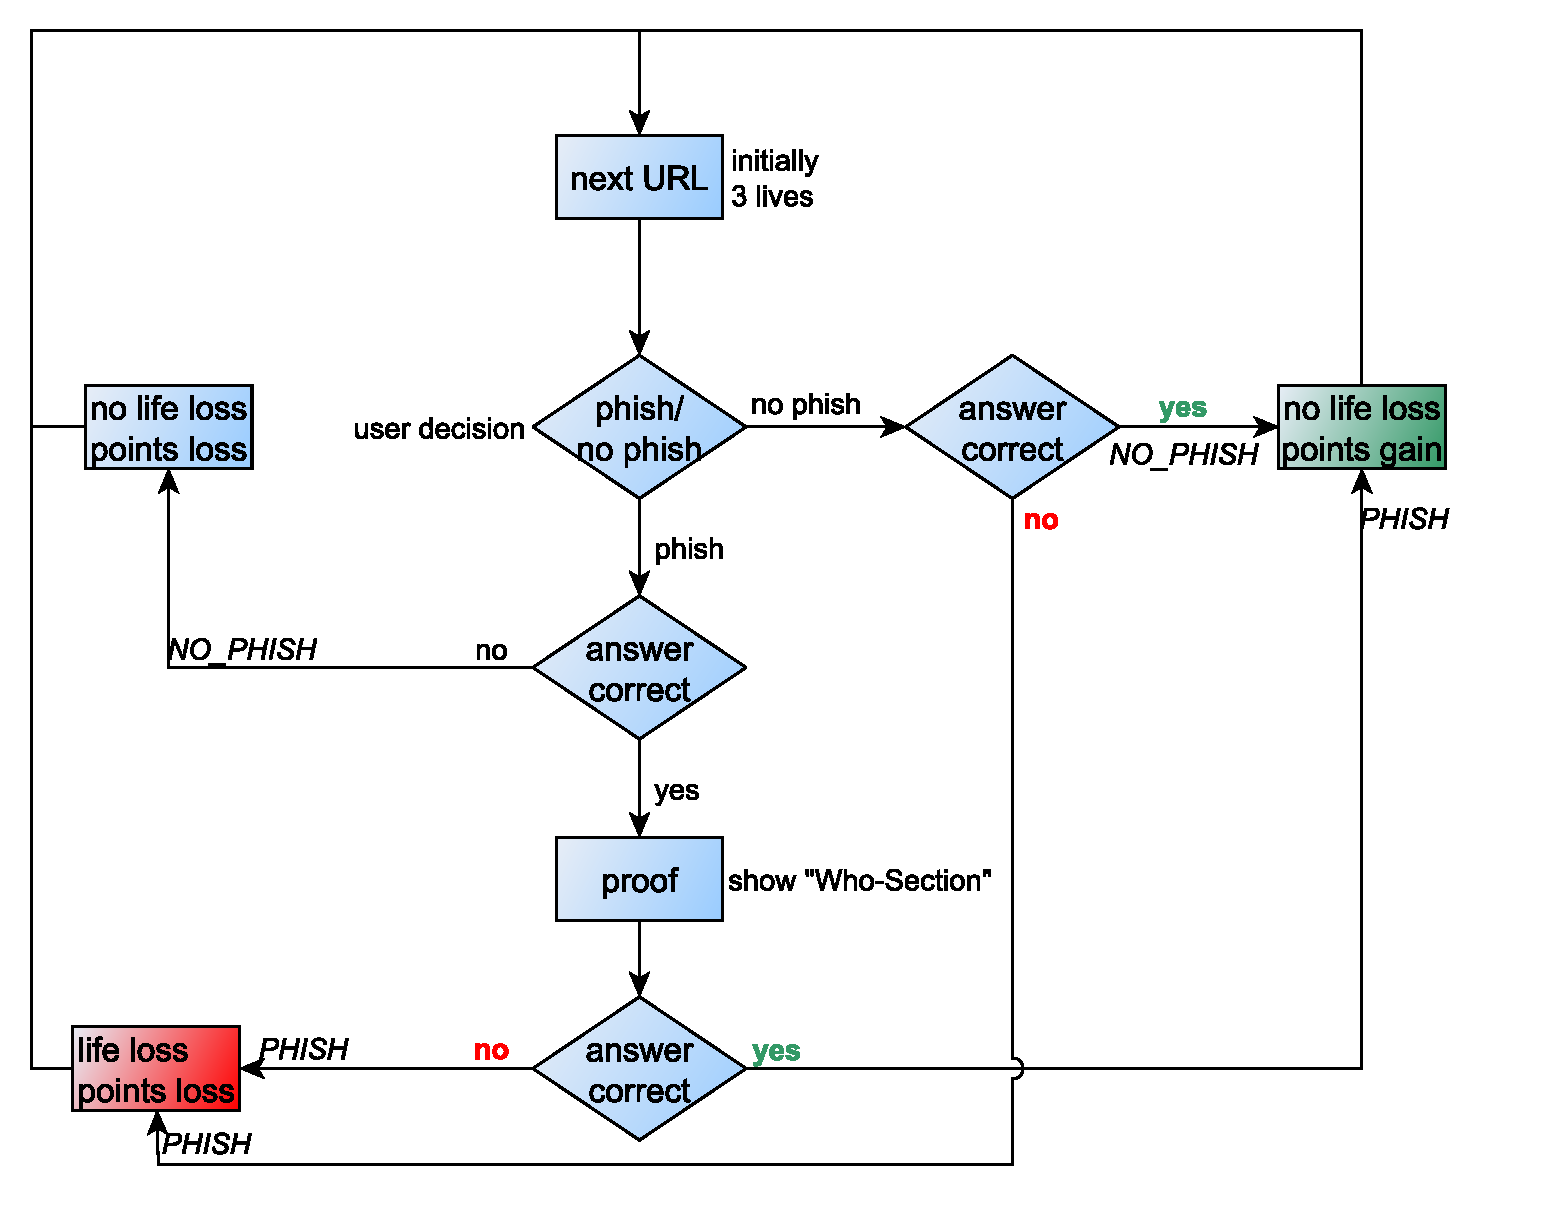
\includegraphics[width=1.0\textwidth]{graphix/lose_win_points.pdf}
\caption{Losing points and lives in the game}
\label{fig:lose_points_life}
\end{figure}
%===========================================
\subsection{Leveling Strategy}
%===========================================
During the app development we have tried out several leveling strategies.
 This section is intended to introduce the leveling strategies we have considered for the app.


\begin{description}[leftmargin=0cm]
	\item[Leveling Based on Achieved Points] Our very first leveling strategy was based on the achieved points per level.
 Each level the user had to achieve at least 100 points to pass the current level and unlock the next one.
 This approach had a major drawback.
 The fact that achieving a minimum of points to pass the level resulted in very similar points for everybody finishing a level.
 That is to say, everybody who has finished level x, has approximately the same points, which in turn would have meant that the comparison between single users would not be meaningful as it would only differ very slightly.
 Additionally, with this strategy, users might replay early levels which are easier and gain the same amount of points as users playing later levels.
 This might result in users playing early levels repeatedly get more points than users playing later and difficult levels.

	\item[Leveling Based on Detected Phishes] The previously described leveling strategy had the deficit of comparability among the users.
 However, we consider comparability very important  since it serves as an incentive for the user to play better or play on.
 For this reason we overthought our strategy and decided that passing a level should not depend on the points a user receives.
 It rather should depend on the number of phishes the user was able to detect during a level.
 That is to say, among the shown URLs in every level there is a certain amount of phishes the user has to detect in order to pass the level.
 With this approach however, there is still the possibility for a user to repeat early, and thus easy, levels and possibly gain more points than users playing later, and thus more difficult, levels.
 To prohibit this, in increasing levels the users gains and loses increasing points accordingly.
 In this way, a user repeating early levels is not able to catch up other users of higher levels.
 This strategy solved the problems of our first strategy, however it also brought a new one.
 The strategy of passing the level when a certain amount of phishes are detected has the following flaw: always rejecting a URL will eventually result in passing the level (if the user also correctly identifies the ``Who-Section'' when required). The user will not gain a lot of points with this strategy, however he will eventually win, which is suboptimal for a game.
  
	\item[Leveling Based on Correct Answers] To solve the problem of our second leveling approach we have extended the leveling passing to correct answers.
 Instead of detecting a certain amount of phishes per level, the user has to give correct answers to a predefined amount of phishing URLs as well as a predefined amount of valid URLs in order to pass the level.
 Only and only if the user has answered the predefined number of valid and phishing URLs the level is completed.
 To additionally incentivize the users we have included three lives per level.
 The lives are supposed to prevent a user playing eternally, without ever passing the current level.
 When the user loses all of his lives, cf.
~Figure~\ref{fig:lose_points_life}, this is an indication that he did not understand what the level is about.
 Consequently, he has to restart the level by being forwarded to the introductory part of the current level.
 This is our final leveling strategy for the app.

\end{description}


%===========================================
\subsection{Teaching Goals Per Level}
%===========================================
\label{s:knowledgetransferperlevel}
This section summarizes the learning objectives of each level.
 Note that we generally do not use technical terms like URL, domain, subdomain, protocol or the like. Figure~\ref{fig:level_teaching_goals} illustrates and exemplifies the level flow of our app.


\begin{description}[leftmargin=0cm]
	\item[Introduction 1] This part is the awareness part described in Section~\ref{s:app_design}. Here, the user learns how easy e-mail spoofing is.
 Additionally, the user is informed about the simplicity of setting up fake websites and that he should not trust the texts of the links he is clicking on.

	\item[Introduction 2] In this part the user is explained how he can access the URL of a web browser and how exactly he has to look at the whole URL.
 In particular, the user is told that he has to scroll up the whole website to make the generally hidden address bar re-appear.
 Then he has to tap the text field of the address bar and scroll to the start of the URL.
 At the end of the exercise for this the user is told that he always has to analyze the URL like this, because all other displayed URLs or links might be fake too.

	\item[Level 1] The actual game starts with level 1, where the user learns about the structure of a URL.
 First of all, the user gets an overview of the single components of a URL.
 To make the comprehension of these components easier to understand we used an analogy which is summarized in Figure~\ref{fig:url_components} with an example URL.
 We told the user that he has to imagine that the website he is visiting is his dialog partner.
 The user is told that the section between ``http(s)://'' and the third slash ``/'', i.
e.
 the hostname, reveals information about his dialog partner.
 In particular, we explain that he has to read this part from right to left.
 The top-level and second-level domain is introduced as ``Who-Section'' (company + location of company), from which the user knows who he is actually talking to.
 All succeeding parts in this area are to be considered as ``departments'' of the company of ther user's dialog partner.
 The protocol part is introduced as ``Security Level'' of the dialog with the partner and the path part of a URL, i.
e.
 the part after the third slash ``/'', is introduced as the topic of the conversation with the dialog partner.
 When marking parts of a URL we consistently used the according colour of Figure~\ref{fig:url_components}. The main objective of the level 1 exercise is to be able to identify the second- and top-level domain of a URL.

	\item[Level 2] With level two we start introducing the spoofing tricks of a phisher.
 We considered the subdomain attack, cf.
~Section~\ref{s:url_categories}, as a good starting point to introduce the phisher as the user has just learnt about the importance of the ``Who-Section'' (top-level and second-level domain) in level 1.
	\item[Level 3] In level 3 the user is first told what an IP address is.
 To facilitate the comprehensibility, we used the analogy of house addresses.
 The user is explained that like addressing our houses with street names and numbers, computers in the Internet are addressed by so called IP addresses.
 The IP address itself is defined as a 4-place sequence of numbers, separated by dots.
 Finally, the user is warned against URLs with IP addresses in the host part.

	\item[Level 4] In this level we deal with nonsense in the second-level domain, cf.
~Section~\ref{s:url_categories}.
	\item[Level 5] In this level we deal with second-level domain names which sound trustworthy, but are in fact unrelated to the company name, cf.
~Section~\ref{s:url_categories}.
	\item[Level 6] Here misleading and deceiving names in the second-level domain of a URL are covered.
 This includes typos, scrambled letters or other similar and deceptive names in the second-level domain, cf.
~Section~\ref{s:url_categories}.
	\item[Level 7] In this level we focus on homographic attacks, where the user is able to visually distinguish a fake second-level domain from the original one, cf.
~Section~\ref{s:url_categories}.
	\item[Level 8] In this level the user is introduced to an attack where the brand name of the visited website or even the whole legitimate URL is placed in the path of a fake URL, cf.
~Section~\ref{s:url_categories}.
	\item[Level 9] Here we introduce the difference between the usage of http:// and https://. In particular, the user is told that the usage of https:// means that his conversation with the website is encrypted and that the dialog partner indicated in the ``Who-Section'' is authenticated.
 As an analogy we say that the https:// represents a higher security level.
 This means, the conversation cannot be eavesdroppbed by a third party and the dialog partner indictated in the ``Who-Section'' has proved his identity to a trusted third party.
 With http:// this security level is not established.

	\item[Level 10] This level does not include an exercise.
 It mainly serves as a section with some important additional input for the user.
 Specifically, we tell the user two things: First, we explain to him that he might encounter URLs which actually look very phishy.
 In such a case, we suggest him to directly contact the company and ask for the authenticity of the specific website.
 Furthermore, we introduce extended validation certificates.
 We provide the user with a link to further information to this subject.

\end{description}

\begin{figure}[hHtbp]
\centering
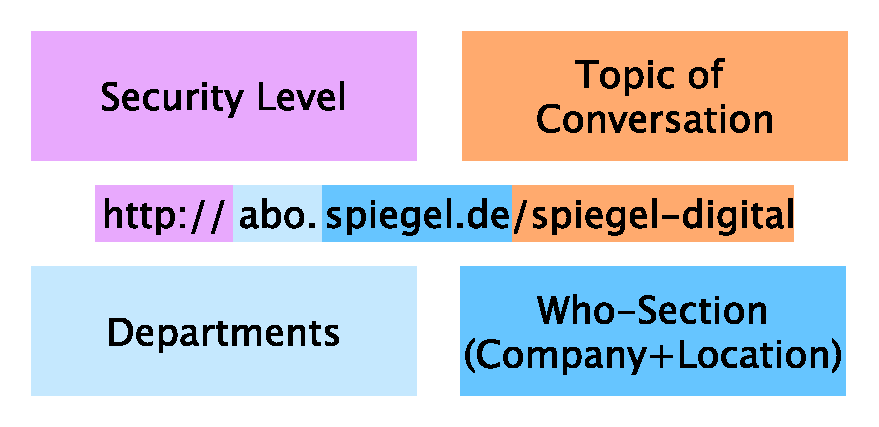
\includegraphics[width=0.56\textwidth]{graphix/url_components.pdf}
\caption{URL components that are communicated to the user}
\label{fig:url_components}
\end{figure}

\begin{figure}[hHtbp]
\centering
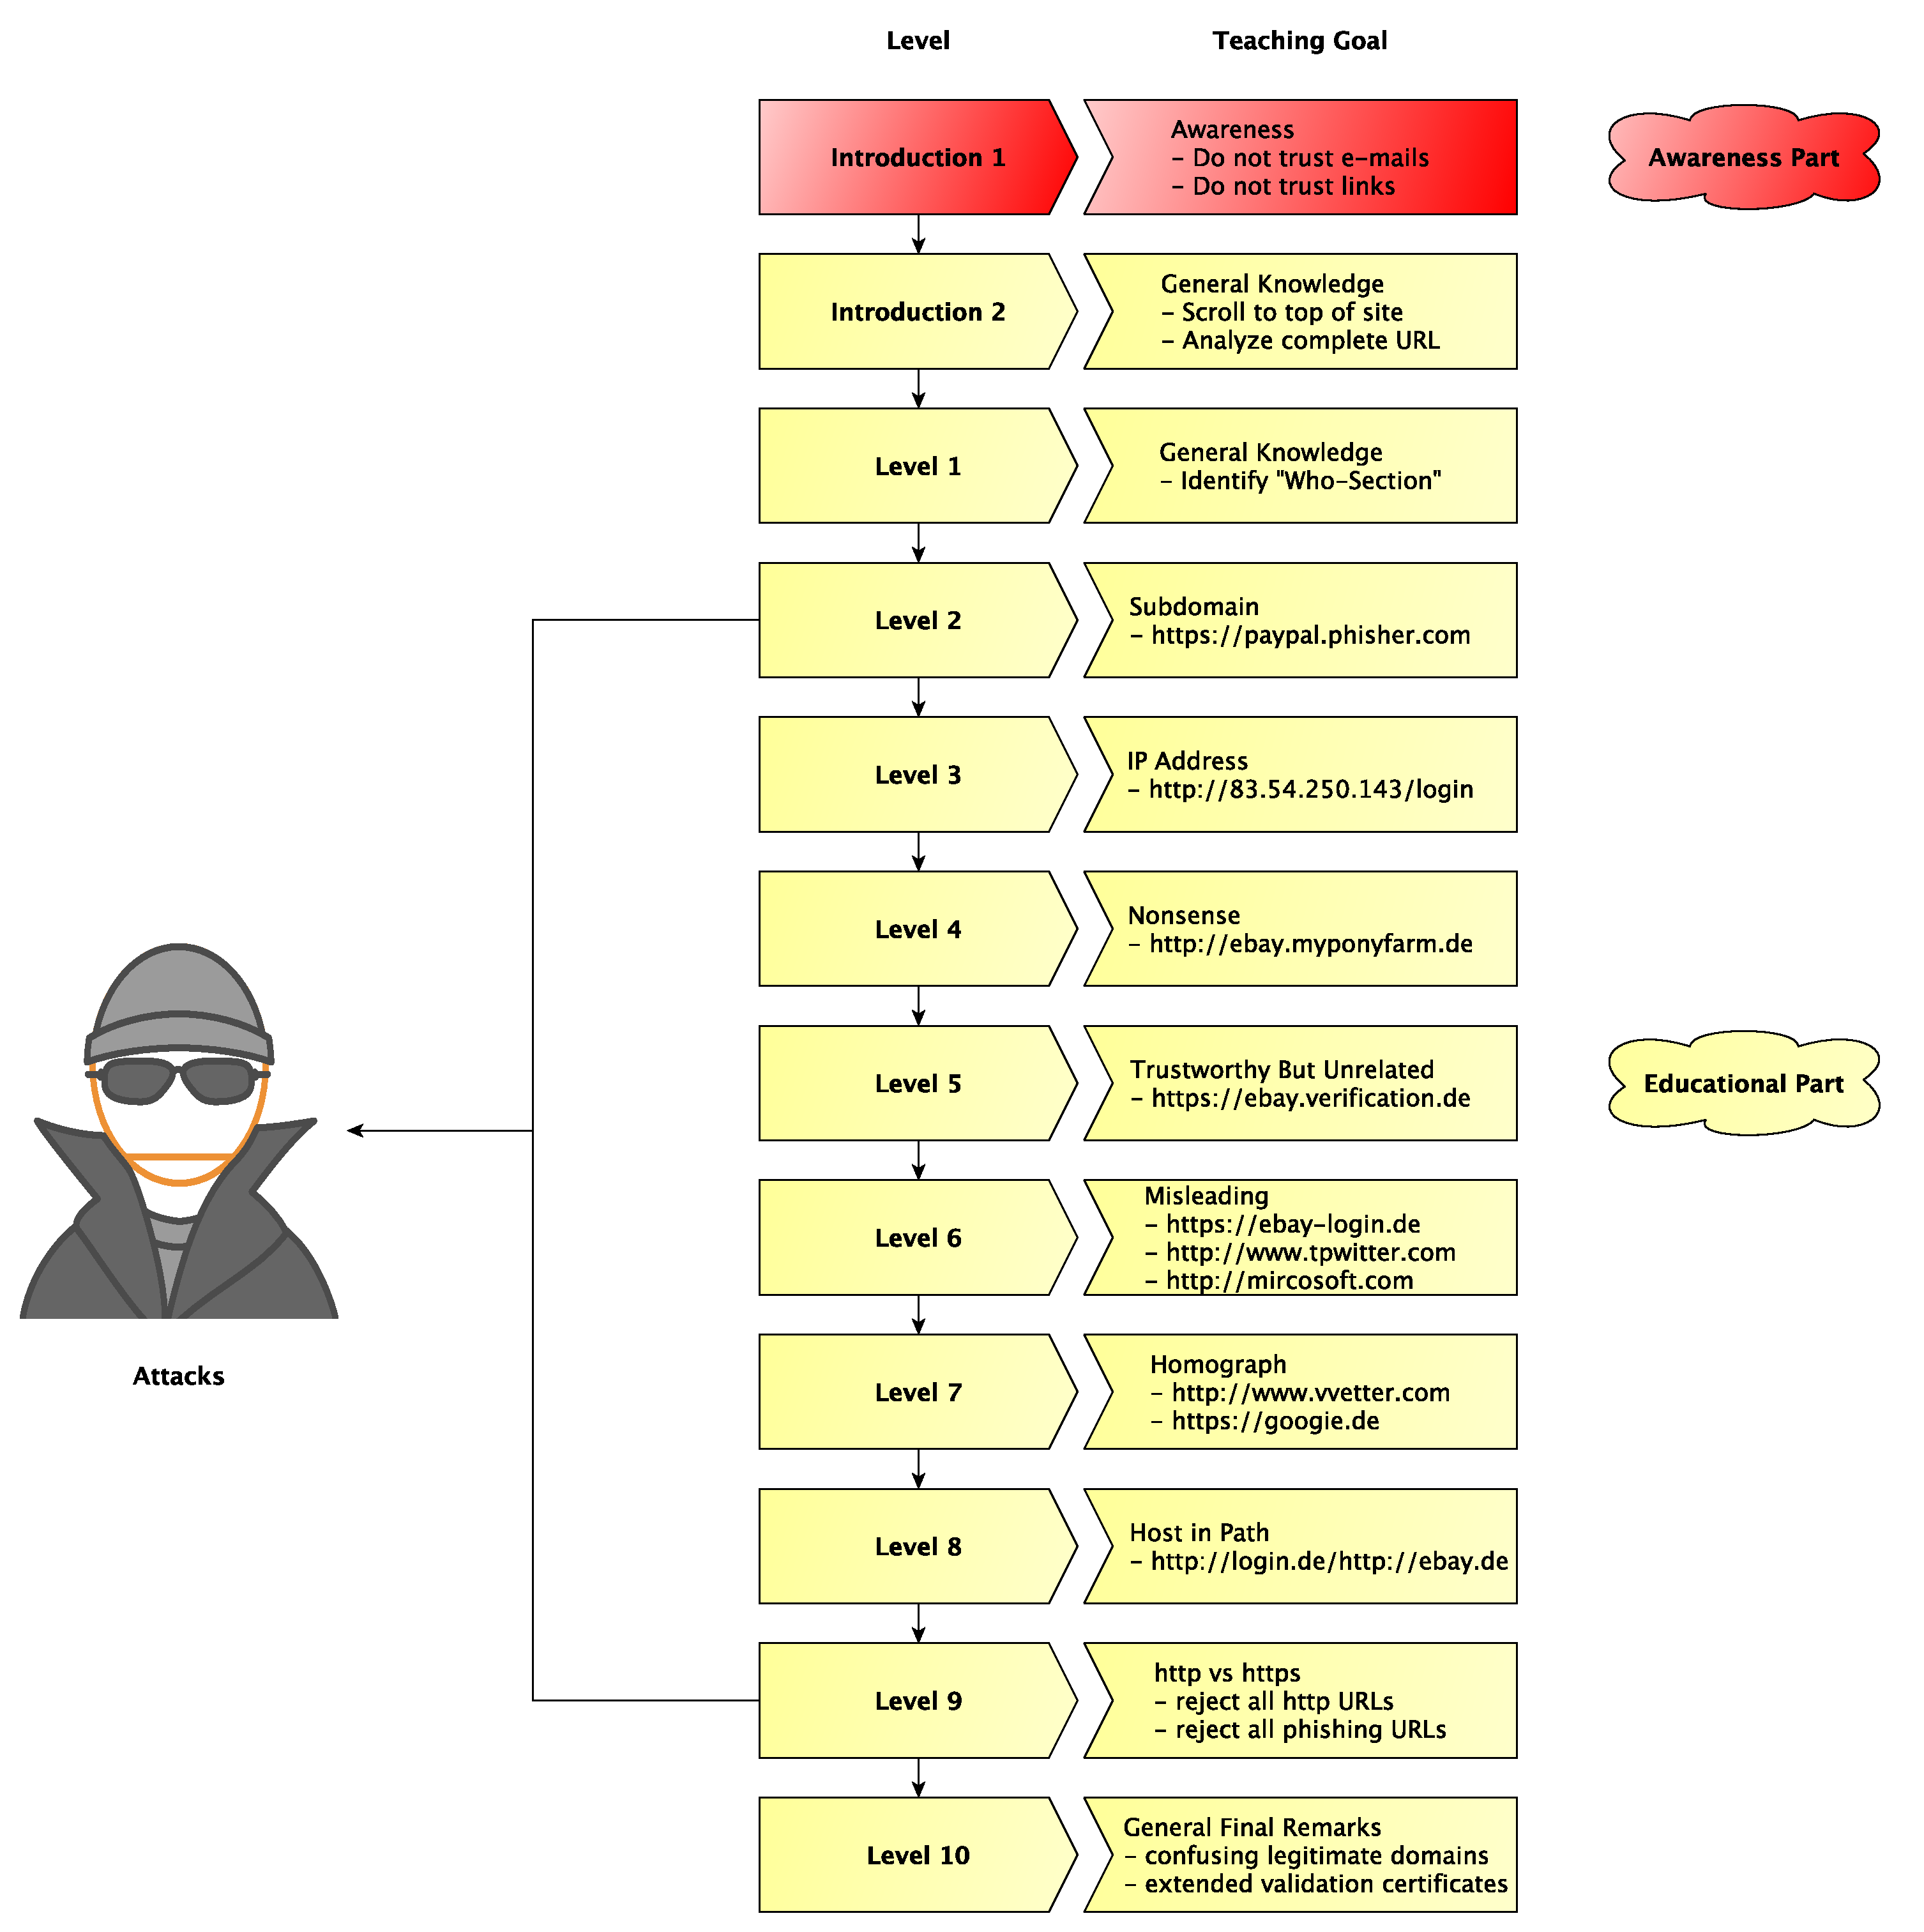
\includegraphics[width=1.0\textwidth]{graphix/level_teaching_goals.pdf}
\caption{Teaching goals of the app}
\label{fig:url_components}
\end{figure}
%===========================================
\subsection{URL Generation}
%===========================================
While playing the app the user is presented with URLs that he has to categorize as phish or valid.
While reviewing the previous works and games in this area we found that many of them use a fixed set of examples.
On some games this set is very small and therefore you are always confronted with the same URLs.
As we layed out in Section \ref{s:url_structure} we want to teach the user how to detect phishing URLs in general.
To accomplish this goal we think that it is essential that the user sees as much different URLs as possible so he can build his own mental model.
Therefore we decided on generating URLs rather than composing a fixed list.
We will lay out the general process here and cover interesting parts of it in the following sections.
\begin{description}
\item[generate attacks for level]When starting a new level we generate a list of Attacks that we want to show the user.
\item[select valid URL]When we want to show a new URL to the user we first select a valid URL from a given set.
\item[apply generator]Then we apply a generator to the URL that does not invalidate the URL but modifies it.
\item[apply attack]After that we select a random attack from the previously build list and apply it to the URL.
\item[repeat]There are combinations of base-URL and attack where the attack doe's not alter the URL.
Therefore it would be impossible for the user to detect the Attack.
In this situation we repeat the process until we find a matching URL.
\end{description}
\subsubsection{generate attacks for level}
\textbf{Was zur historie?}
The types of URLs the user is presented is dependent on the level.
Each level introduces on or more attacks.
Which attack is introduced in which level is layed out in section\ref{s:knowledgetransferperlevel}.
In general the URLs of each level $n$ are distributed as follows:
\begin{table}[hHtbp]
\centering
\begin{tabular}{llll}
Total number of URLs&$u$&$6+2*n$&starting with 6 URLs each level has 2 more URLS.\\
Number of Phishes&$p$&$u/2$&Half of the URLs are phishes.\\
Number of repeats&$r$&$\left\lfloor p/2 \right\rfloor$&Half of the phishes are repeats.
\end{tabular}
\caption{distribution of URLs per level.}
\label{t:levelurls}
\end{table}

The repeats are always one attack from each previous level. The rest of the repeats is filled up randomly.

There are two main exception to these rules:
\begin{description}
\item[Level 1] In Level 1 the game is modified in the form that the user is only presented with valid URLs and has to select the domain.
To prevent boring the user in this level we only present 5 URLs.
None of them is a phish.
\item[Level 1+2] The first level that contain repeats is level 3 because level 2 is the first real game level.
\end{description}

The generated list of attacks also contains a special attack that does no real attack. This is to simplify the URL generation. When we generated the list of attacks we save it for later reference.

\subsubsection{select valid URL}
When we want to present the user URL we start by selecting a valid URL from a given set.
To build this set we used Alexa\ref{alexa} to find the top 100 domains for german users.
We then went to each of these sites and by navigating tried to find 6 URLs for each domain.
We tried to find some short and some long URLs.

	
%===========================================
\section{Development}
%===========================================
This chapter deals with the development process of our app.
We do not provide in-depth insight to our source code. 
Instead we give a brief overview of our approach for the development of a user friendly and understandable app.
%===========================================
\subsection{Mock Up}
%===========================================
After we have decided about the work flow and structure of our app we built a mock up in order to get a more concrete idea of what needs to be implemented and to reveal flaws in our thought process.
Also, we showed it to a couple of friends and relatives so we could expose aspects we have not yet thought about.
All in all, the work flow and structure of the mock up was quite understandable.
However, the first texts explaining how to access the address bar and about the structure of a URL seemed to be incomprehensible.
As a consequence, we adjusted these texts in the app (only thos of the first three levels) and showed them to other friends and relatives who seemed to understand the descriptions.
Based on these initial texts we wrote all remaining texts without including it into the app yet.
The next section deals with the elaboration of these texts.
%===========================================
\subsection{App Texts}
%===========================================

%===========================================
\subsection{Pilot Study}
%===========================================
%===========================================
\subsection{URL Generation}
%===========================================
While playing the app the user is presented with URLs that he has to categorize as phish or valid.
While reviewing the previous works and games in this area we found that many of them use a fixed set of examples.
On some games this set is very small and therefore you are always confronted with the same URLs.
As we layed out in Section \ref{s:url_structure} we want to teach the user how to detect phishing URLs in general.
To accomplish this goal we think that it is essential that the user sees as much different URLs as possible so he can build his own mental model.
Therefore we decided on generating URLs rather than composing a fixed list.
We will lay out the general process here and cover interesting parts of it in the following sections.
\subsubsection{Example URLs}
To present attacked URLs to the user we found int most realistic to take valid URLs and apply attacks on them.
Therefore we needed a set of valid URLs.
To build this set we used Alexa\ref{alexa} to find the top 100 domains for german users.
We then went to each of these sites and by navigating tried to find 6 URLs for each domain.
We tried to find some short and some long URLs.
\begin{description}
\item[generate attacks for level]When starting a new level we generate a list of Attacks that we want to show the user.
\item[select valid URL]When we want to show a new URL to the user we first randomly select a valid URL from the before mentioned set.
\item[apply generator]Then we apply a generator to the URL that does not invalidate the URL but modifies it.
\item[apply attack]After that we select a random attack from the previously build list and apply it to the URL.
\item[repeat]In some situations we need to try again.
\end{description}
\subsubsection{generate attacks for level}
\textbf{Was zur historie?}
The types of URLs the user is presented is dependent on the level.
Each level introduces on or more attacks.
Which attack is introduced in which level is layed out in section\ref{s:knowledgetransferperlevel}.
In general the URLs of each level $n$ are distributed as follows:
\begin{table}[hHtbp]
\centering
\begin{tabular}{llll}
Total number of URLs&$u$&$6+2*n$&starting with 6 URLs each level has 2 more URLS.\\
Number of Phishes&$p$&$u/2$&Half of the URLs are phishes.\\
Number of repeats&$r$&$\left\lfloor p/2 \right\rfloor$&Half of the phishes are repeats.
\end{tabular}
\caption{distribution of URLs per level.}
\label{t:levelurls}
\end{table}

The repeats are always one attack from each previous level. The rest of the repeats is filled up randomly.

There are two main exception to these rules:
\begin{description}
\item[Level 1] In Level 1 the game is modified in the form that the user is only presented with valid URLs and has to select the domain.
To prevent boring the user in this level we only present 5 URLs.
None of them is a phish.
\item[Level 1+2] The first level that contain repeats is level 3 because level 2 is the first real game level.
\end{description}

The generated list of attacks also contains a special attack that does no real attack. This is to simplify the URL generation. When we generated the list of attacks we save it for later reference.
\subsubsection{apply generator}
We were unsure if we still have enough valid URLs so we prepared a way to automatically modify the URLs in such a way that they could still be valid URLs. Some Ideas where to add subdomains or path strings to the URL. Query or fragments are also possible. We later found out that it is currently not needed to implement generators because there are a lot of URLs in our set. If however we will some time in the future find out that these URLs are not enough we have this scheme in place.
\subsubsection{apply attack}
After we generated a valid URL we chose a random attack from the previously build set of attacks and apply it to the URL. With this we also store which attack we currently applied. This is important when the user is failing this round. In this situation we will simply readd this attack to the set of attacks.
\subsubsection{repeat}
There are combinations of base-URL and attack where the attack doe's not alter the URL.
Therefore it would be impossible for the user to detect the Attack and he will be confused and might stop using the app.
In this situation we repeat the whole URL generation process until we find a matching URL.
	%*******************************************
\section{App Evaluation}
%*******************************************
\label{s:evaluation}
After having designed and implemented the app, the evaluation of our work remains as a final step. This chapter describes our evaluation process.
 The app will be evaluated with the aid of a user study.
 After introducing our study design, we will state our hypotheses and explain how we are going to measure our statements.
 Finally, we will analyze our results and state our conclusion.


%===========================================
\subsection{Participant Recruitment}
%===========================================
\label{s:participant_recruitment}
This section deals with the participant recruitment for the user study.
As an incentive to attend our user study a gift card was raffled among 4 users.
A major challenge was not to address close friends in order to receive unbiased and honest feedback. 
To reach potential participants we proceeded as follows:

\begin{description}[leftmargin=0cm]
\item[Flyer:]  We prepared a flyer with the most important information. 
In this flyer we told the user that a learning app about Internet security in general will be tested. 
We did not mention the specific topic of phishing in advance because we did not want potential participants to read up about it before the study.
Copies of this flyer were hung on blackboards of student dorms and some other buildings at the university.
\item[E-Mail to Professors:] We additionally distributed the flyer to a number of professors in our university and asked them to forward it to their students and/or teaching staff.
We did not forward the flyer to computer science professors or professors of similar technical majors since their students and staff most likely do not match our target group.
\item[Online Social Networks:] We contacted our friends in online social networks and asked them to ask friends whether they would be willing to participate in our user study.
Additionally, we posted the flyer in university groups of online social networks with the hope some people might be interested in participating.
\item[Further Networks:] Finally, we called friends we could not reach via online social networks and asked them if they knew anybody who would participate.
\end{description}
In \autoref{s:participant_recruitment_texts} copies of our e-mails to the professors and of our flyer can be consulted.
Note that we had to split the user study into groups of 4 participants due to the lack of available smartphones.
Moreover, our flyer originally said that the best participant of each group would win the gift certificate.
However, we recognized that the winning chance might not be equal for every participant due to varying expertise, for example, or other possible technical problems such as app crashes.
For this reason we asked the participants at the beginnig of each study whether they agreed to raffle the gift certificate instead.
To express our appreciation to each participant we decided to offer cookies and other kinds of sweets.
Additionally, the participant who performed best was awarded with a ``Golden Anti-Phish Certificate'', all other participants received a ``Silver Anti-Phish Certificate'' (cf. \autoref{s:antiphish_certs}).

%===========================================
\subsection{Study Design}
%===========================================
For our user study we chose a within-subject design, i.e. a ``before and after app'' study with the same group of people.
The advantages of this design can be summarized as follows:
Within-subject deals better with variability associated with individual differences compared to between-group design, where different groups would be considered who do and do not play the app.
A major drawback of the within-subject design, however, is the learning effect.
We are not able to clearly distinguish whether a behavior change after playing the app is a result of the app intervention or of learning effects.
Yet, our results showed that the learning effects seemed to have only a minor impact (cf. \autoref{s:hypanalysis}).

\autoref{fig:study_structure} illustrates the structure and process of our study. In the following, we dwell on each of the consecutive steps:
\begin{enumerate}
	\item \textit{Informed Consent:} Before starting the user study the participants have to sign an informed consent.
This form briefly explains what the study is about and clarifies that the participant is not obliged to finish the study.
If the user terminates the study before finishing it, however, he cannot participate in the gift certificate raffle.
Optionally, the user can agree with the anonymous publication of the:
	\begin{enumerate}
		\item transcriptions of the study (recordings will be deleted after the study)
		\item filled out surveys
	\end{enumerate}

	\item \textit{General-Survey Before:} At the beginning the participants have to fill out a general survey, where they have to judge their own knowledge on the topic of Internet security in general.
 For instance, they are asked whether it is easy for them to distinguish legitimate e-mails and websites from fake ones.

	\item \textit{Website-Survery Before:} In this part of the user study the participants get a list of screenshots of websites.
 The screenshots had been taken with the standard browser of an Android tablet.
 In total, the user is shown 16 screenshots, with 8 phishing and 8 valid URLs.
 The user has to decide whether he would enter confidential data on the shown website.
 Additionally, he has to encircle the part of the screenshot which was the primary reason for his decision.
 Then, the user has to indicate how sure he was about his answers on a Likert scale.
 Finally, the user is asked whether he knows the vendor of the website and whether he has an account there.

	\item \textit{Play App:} Here, the users get the smartphones in order to play the app.
 To save time, we skipped the introduction 2 part (how to access the address bar) for the user study.
 The user has half an hour to play.
 Afterwards, they are asked to put the smartphones aside.
 Then, we collect the smartphones and note the reached points for each level.

	\item \textit{Website-Survery After:} After playing the app, the participants get a second website-survey.
 In this, all examples of the previous survey are included.
 Moreover, it contains 8 further website screenshots of which 4 represent phishing and the other 4 legitimate URLs.

	\item \textit{General-Survey After:} Here, the participants are asked to complete a form with questions pertaining to their person, for example, their age or course of study.
 This form does also contain questions related to the System Usability Scale (SUS)~\cite{sus}, which is supposed to assess the usability of our app, and questions regarding the users' impression of the app.
	
	\item \textit{Certificates:} At this point the official part of the study is finished.
We thank the users for their participation and award a ``Golden Anti-Phish Certicate'' to the best participant of the current group.
All other attendants receieve a ``Silver Anti-Phish Certificate''.
Next, the gift certificate is raffled.

	\item \textit{Debriefing:} After the official end of the study (after handing out the certificates) we asked the participants if they were willing to stay for an optional debriefing, where they could ask questions or provide their remarks in person. In case a participant did not want to stay for this debriefing, he was free to go.
\end{enumerate}



\begin{figure}[hHtbp]
\centering
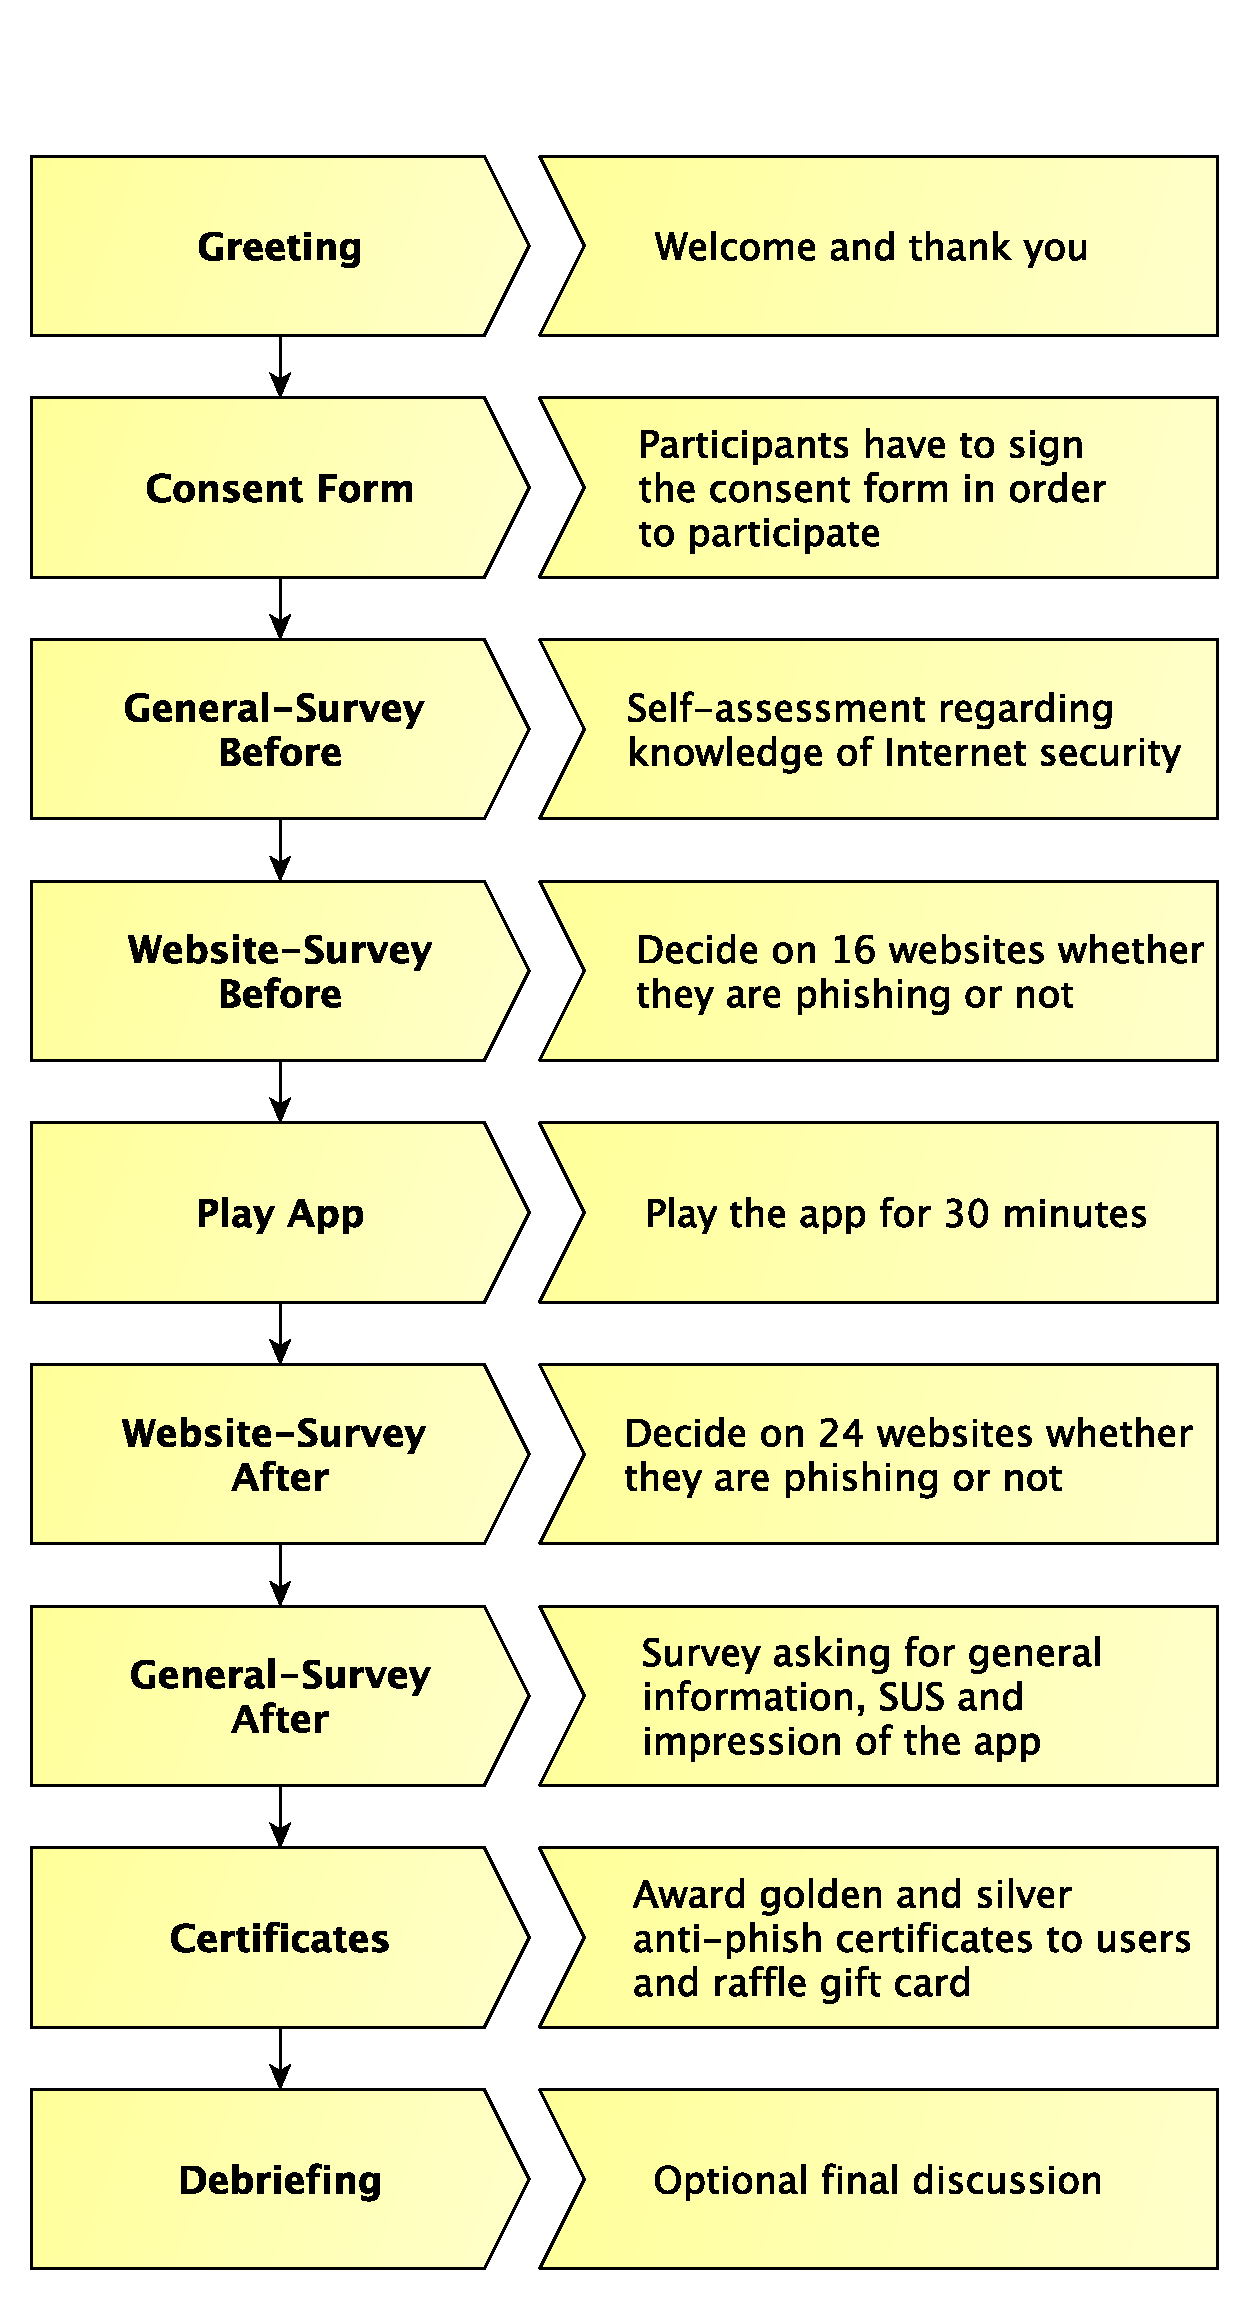
\includegraphics[height=0.9\textwidth]{study_structure.pdf}%
\caption{Structure and process of our final user study}%
\label{fig:study_structure}%
\end{figure}

%===========================================
\subsection{Hypotheses}
%===========================================
In order to evaluate the effectiveness and usability of our app we formulated the following hypotheses and measurements.

\begin{enumerate}
	\item \textit{Hypothesis 1 - Mistakes:} After playing the app, the users make significantly less mistakes when deciding whether a website is a phish or not than before using the app.\newline
	Measurement: Correctly identified websites in ``Website-Survery After'' (phish or no phish) $>>$ correctly identified websites in ``Website-Survery Before''
	\item \textit{Hypothesis 2 - URL Based Decision:} After playing the app, the users primarily base their decision whether a website is a phishing website or not significantly more often on the URL compared to before playing the app.\newline
	Measurement: Number of URL markings in ``Website-Survery After'' $>>$ number of URL markings in ``Website-Survery Before''
	\item \textit{Hypothesis 3 - URL Comprehension:} After playing the app the user understands that the domain of a URL is the most important criterion to detect phishing websites\newline
Measurement: Number of marked URL domains in ``Website-Survery After''  $>>$ number of marked URL domains in ``Website-Survery Before'' 
	\item \textit{Hypothesis 4 - Good Usability:} The usability of the app is above average. \newline
Measurement: A System Usability Scale (SUS) $>$ 68 can be considered above average usability~\cite{sus}.
\end{enumerate}

%===========================================
\subsection{Classifying Markings}
%===========================================
\label{s:markings}
One part of the study involved marking the area on a given website which contributed to the users' decision on whether they thought the website was fraudulent or legitimate.
In order to assess these markings, for the measurement of hypothesis 3, we needed to define respective codings.
Here, we provide an overview of the regions participants marked during the website-surveys and how we coded them internally for the evaluation.
Furtheremore, we discuss our marking interpretations and outline several interpretation problems, due to imprecise markings, and how we approached those.

%.........................................................................................................
\subsubsection{Marking Examples}
%.........................................................................................................
The following list summarizes the codings we used for the markings of the participants.

\begin{enumerate}
	\item\textit{None:} Occasionally, participants did not mark or encircle anything of the screenshot. In our raw data this is coded as none (cf.~\autoref{}).
	\item\textit{Favicon or Padlock:} The marking of a favicon or padlock is trivially coded accordingly (cf.~\autoref{fig:padlock}).
	\begin{figure}[H]
	\centering
	\includegraphics[width=0.8\textwidth]{m_padlock.png}
	\caption{Padlock marked}
	\label{fig:padlock}
	\end{figure}
	\item\textit{Content:} If anything else than the URL itself, a part of the URL, a favicon, or a padlock is marked then this is coded as content (cf.~\autoref{fig:content}).
	\begin{figure}[H]
	\centering
	\includegraphics[width=0.8\textwidth]{m_content.png}
	\caption{Content marked}
	\label{fig:content}
	\end{figure}
	\item\textit{Scheme:} If the scheme or a part of the scheme in a URL is marked, this is coded as scheme (cf.~\autoref{}).
	\item\textit{Host:} Marking the host results in an according coding (cf.~\autoref{fig:m_host}).
		\begin{figure}[H]
		\centering
		\includegraphics[width=0.8\textwidth]{m_host.png}
		\caption{Host marked}
		\label{fig:m_host}
		\end{figure}
	\item\textit{Domain:} In case a participant marks a domain (cf.~\autoref{fig:m_domain}) or the substring of a domain (cf.~\autoref{fig:m_domain_substring}) this is coded as domain or domain substring accordingly.
For the measurement of hypothesis 3, domain as well as domain substring markings are considered domains.
\begin{figure}[H]
\centering
\includegraphics[width=0.8\textwidth]{m_domain.png}
\caption{Domain marked}
\label{fig:m_domain}
\end{figure}
\begin{figure}[H]
\centering
\includegraphics[width=0.8\textwidth]{m_domain_substring.png}
\caption{Domain substring marked}
\label{fig:m_domain_substring}
\end{figure}

	\item\textit{URL:} All other markings are coded as URL and measured as such. For instance, the subdomain of a URL is coded as URL (cf.~\autoref{fig:m_url_02}).
	\begin{figure}[H]
	\centering
	\includegraphics[width=0.8\textwidth]{m_url_02.png}
	\caption{Subdomain marked, coded as URL}
	\label{fig:m_url_02}
	\end{figure}
\end{enumerate}

%.........................................................................................................
\subsubsection{Interpretation Problems}
%.........................................................................................................
\label{s:intprobs}
While assessing and digitalizing our data we had to face some interpretation problems which we exemplify in the following.
In such cases we had no choice but striving to interpret the samples as objectively as possible.
\autoref{fig:m_content_or_host}, for instance, shows a marking where the circle includes the content (YouTube logo) as well as the host. 
For this sample, we decided to code the marking as host.
The next example in \autoref{fig:m_domain_or_not} shows a marking where a subdomain and the domain is marked. 
When we faced examples like this we decided to code it as domain in case a subdomain is only partially marked, so that there is an indication that the user just did not make his markings precise enough.
If the subdomain is obviously marked deliberately, i.e. clearly inside the circle, this kind of sample is coded as URL.
In this case we see that the subdomain is inside the circle and coded this sample as URL accordingly.
Another frequently occurring sample is one where two areas are marked, even though we explicitly asked to mark only one.
In these cases we decided as follows: in case a marking is obviously striking due to a thicker circle, for instance, the more emphasized area is chosen for coding.
In case both markings were equal, we joined the markings and decided based on that.
In \autoref{fig:m_url}, for instance, a participant marked the scheme and the host separately. 
We cannot observe any emphasis on one of the markings.
Therefore, we chose to code this sample as URL.
Finally, there were samples where the user correctly identified a phishing website.
However, instead of marking the domain as the reason (as it is done in the app), some users marked the attacked part instead.
\autoref{fig:m_attack_recognized} illustrates such an example.
In fact, marking the attacked part is justified. 
Yet, we had to code such samples as URL since there is no clearcut way of defining whether an attacked part of a URL was recognized or not.
In the contrary, the domain of a URL can always be considered as the attacked part. Therefore, users should primarily base their decisions on domains.

\begin{figure}[H]
\centering
\includegraphics[width=0.8\textwidth]{m_content_or_host.png}
\caption{Host or content marked?}
\label{fig:m_content_or_host}
\end{figure}

\begin{figure}[H]
\centering
\includegraphics[width=0.8\textwidth]{m_domain_or_not.png}
\caption{Domain or URL marked?}
\label{fig:m_domain_or_not}
\end{figure}

\begin{figure}[H]
\centering
\includegraphics[width=0.8\textwidth]{m_url.png}
\caption{Scheme or host marked?}
\label{fig:m_url}
\end{figure}

\begin{figure}[H]
\centering
\includegraphics[width=0.8\textwidth]{m_attack_recognized.png}
\caption{Attack marked}
\label{fig:m_attack_recognized}
\end{figure}

%===========================================
\subsection{Results and Analysis}
%===========================================
This section presents our results and analyzes them. 
We start with discussing the representativeness of our participants and proceed with illustrating interpretation problems we faced while we assessed the website-surveys.
Therafter, we evaluate our hypotheses and proceed with further exploration of our results, followed by discussing the limitations of our study.
Finally, this chapter concludes with a disussion of our results and a corresponding summary. 
%.........................................................................................................
\subsubsection{Representativeness of Our Participants}
%.........................................................................................................
\label{s:representativeness}
In \autoref{s:target_group_def} we defined preconditions that users have to hold in order to match our target group.
We aspired to recruit participants who hold these preconditions as far as possible.
In the following we discuss the representativeness of our participants with the aid of these preconditions.

\begin{description}[leftmargin=0cm]
	\item[Attackability:] Generally, we took care that the people we recruited do not have extensive prior knowledge on this topic.
For example, our flyer asked for non-specialists.
Yet, we were not able to assure beforehand that we would only have non-specialist participants.
In such a case we had to rule them out for our analysis afterwards.
Unlike in our initial survey (cf. \autoref{s:survey}), we did not exclude electrical engineers or computer scientists in general from our final user study.
The problem with the phishing survey was that it did not give us enough indication whether a particular participant was too familiar with the topic.
Therefore, we had to imply that computer scientists and electrical engineers are too skilled, even if this does not necessarily need to be the case in reality.
In fact, there might be computer scientists or electrical engineers who can learn something from our app.
In contrast to the phishing survey, in our final user study we were able to determine a user's prior knowledge more precisely with the aid of the website-survey before.
Therefore, we did not primarily consider their course of study or field of work, but rather how well they performed in the website-survey before playing the app (cf. \autoref{s:hypanalysis}).
This way we assured that the considered participants were potential targets of phishing.
	\item[Android Users:] For the study we considered it important that our participants own a smartphone in general since we wanted the focus to be on our contents. This way, we minimize failures resulting from general operating difficulties.
Since we provided the required smartphones during the study we had no need to recruit participants who obligatorily own an Android smartphone.
	\item[Language:] Participants of our study need to know German because all of the app texts are in German. This was ensured by providing flyers and e-mails in German language so that persons who do not master the German language do not feel to be addressed.
All of our participants could speak and read German.
\item[Motivation:] We mainly target users who download our app by choice and thus have a basic motivation to learn something from it.
For the user study our flyer was supposed to draw interested persons to participate in our study.
Furthermore, we created an additional incentive to attend our study by raffling a gift certificate.
\end{description}
Finally, we aspired to recruit participants who are not close friends of ours in order to minimize biases as far as possible.
%.........................................................................................................
\subsubsection{Analysis of Our Hypotheses}
%.........................................................................................................
\label{s:hypanalysis}
In total 19 participants attended our study.
As discussed in \autoref{s:representativeness} we did not rule out any participant beforehand because by means of the website-survey before we were able to precisely determine the prior knowledge of the participants.
Ultimately, we had to sort out two participants for the results and analyses of our study:

\begin{enumerate}
	\item\textit{Outlier:} \autoref{fig:outlier} depicts the performance of our participants.
	It illustrates how many URLs were correctly identified by how many users.
	Evidently, there is an outlier among our participants. 
	One user gave 15 correct answers to 16 questions.
	Thich means that he has too much prior knowledge on this topic and thus does not match our target audience.
	Therefore, this participant is not considered for our further elaborations.
	\item\textit{Seriousness:} Another participant obviously did not engage himself to play our app.
	During the 30 minutes of playing the app the user managed to complete the awareness part and level 1 (identify domain) only.
	More importantly, we saw the user playing around with the Samsung device instead.
	Since this user did not seem to take our study and app seriously we decided to sort him out for further considerations.
\end{enumerate}

\begin{figure}
\centering
\subfigure[Before]{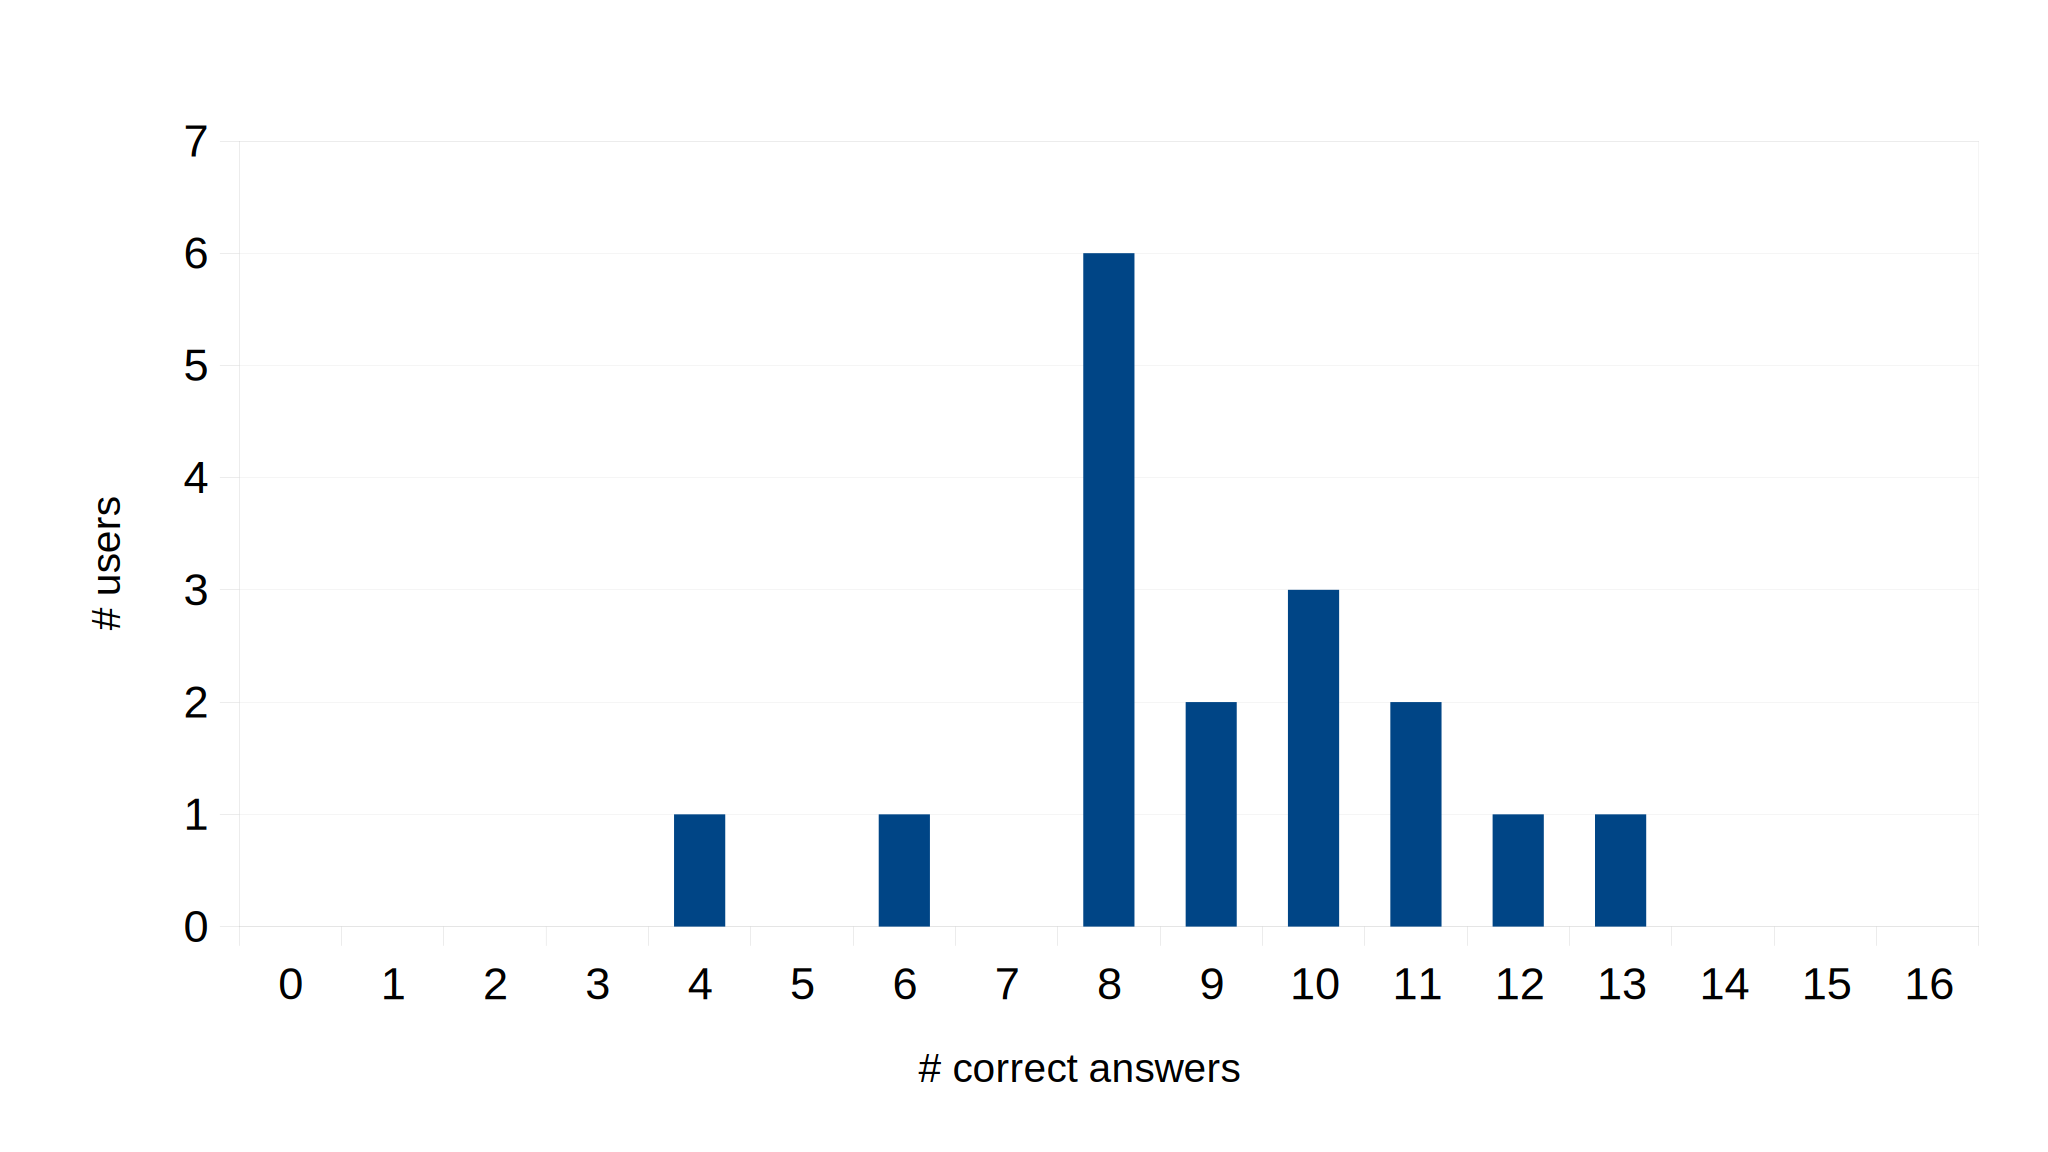
\includegraphics[width=0.45\textwidth]{hyp1b.pdf}}
\subfigure[After (all URLs)]{\label{fig:hyp1resultsaall}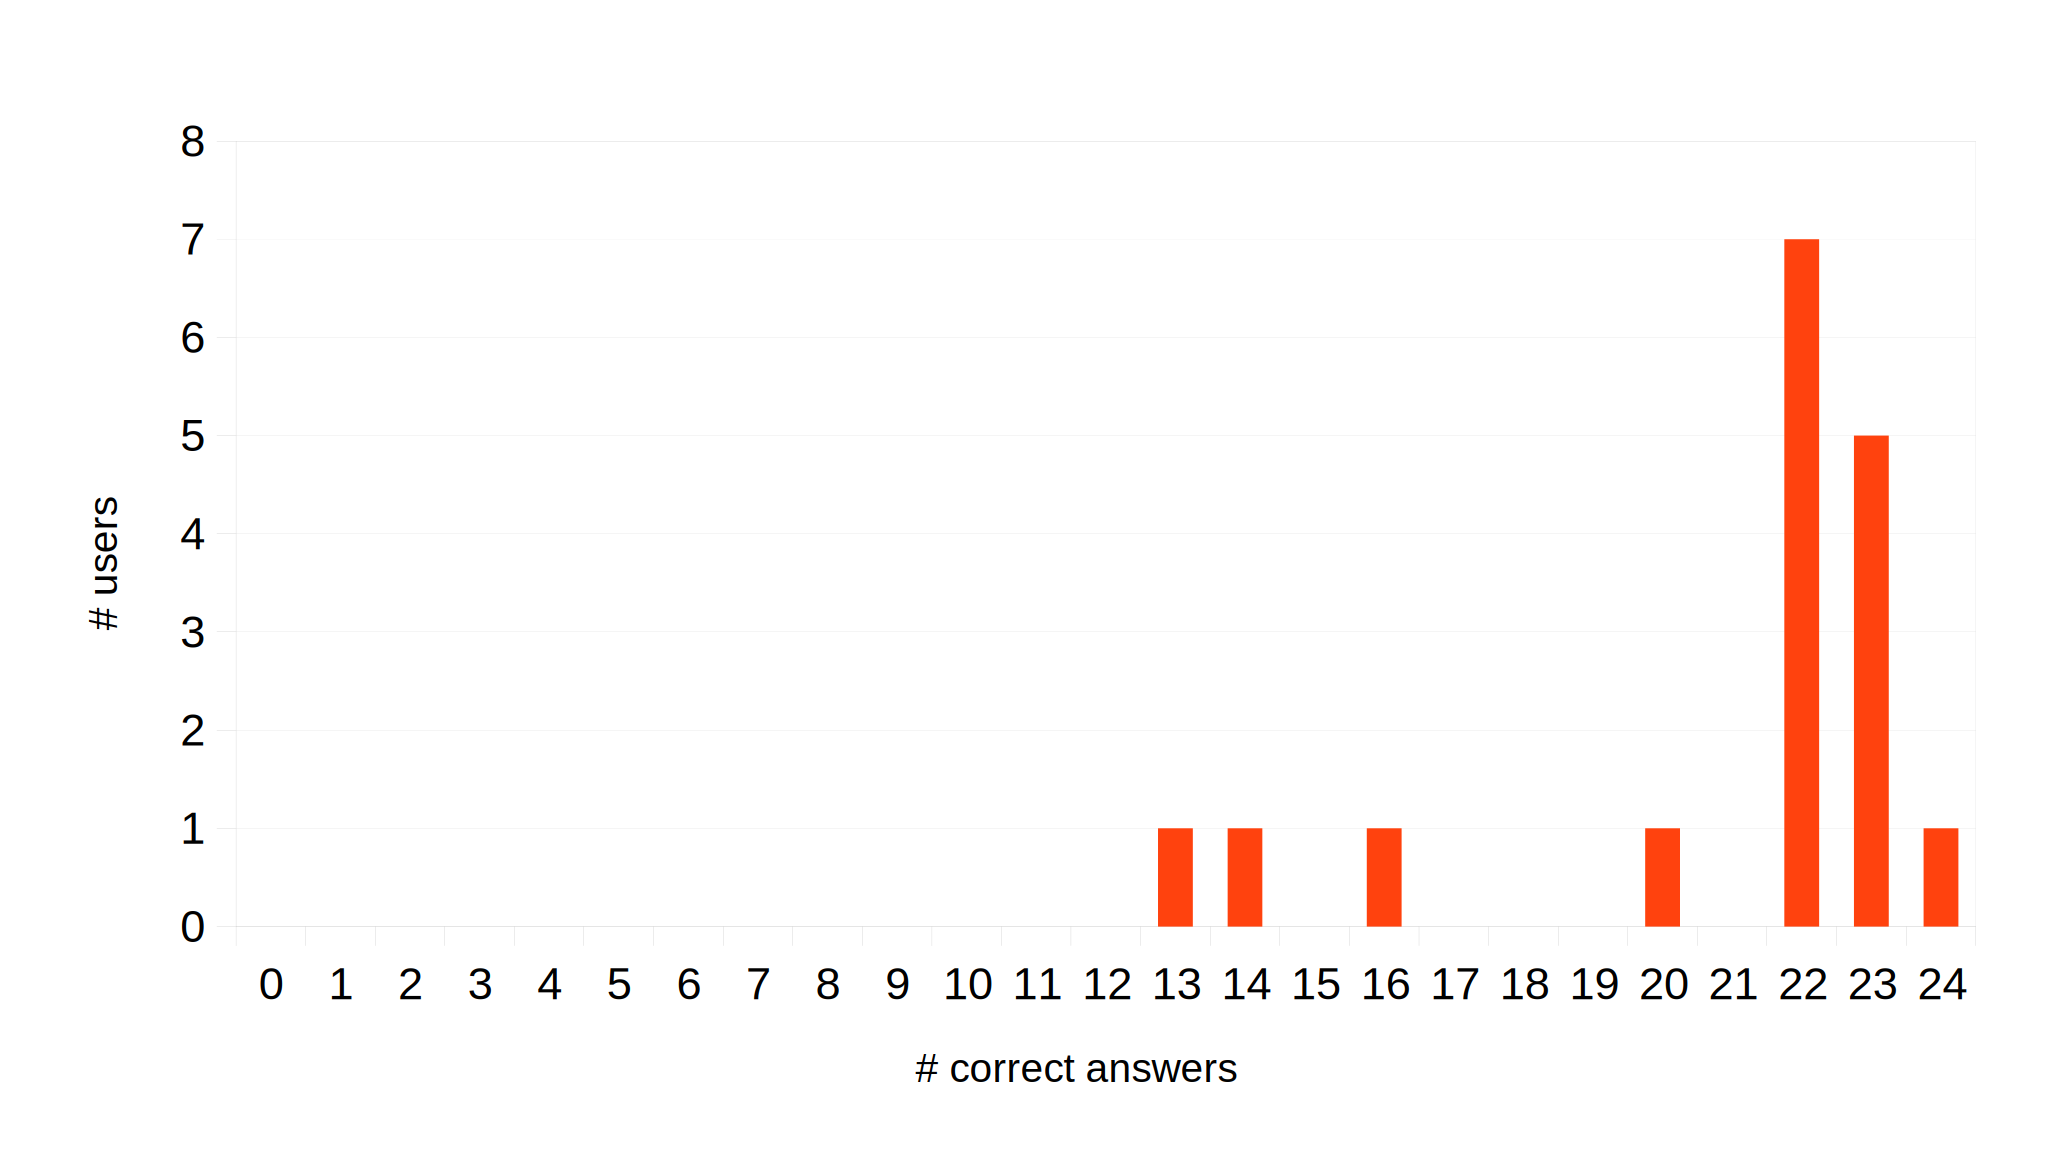
\includegraphics[width=0.45\textwidth]{hyp1a.pdf}}
\subfigure[After (New URLs)]{\label{fig:hyp1resultsanew}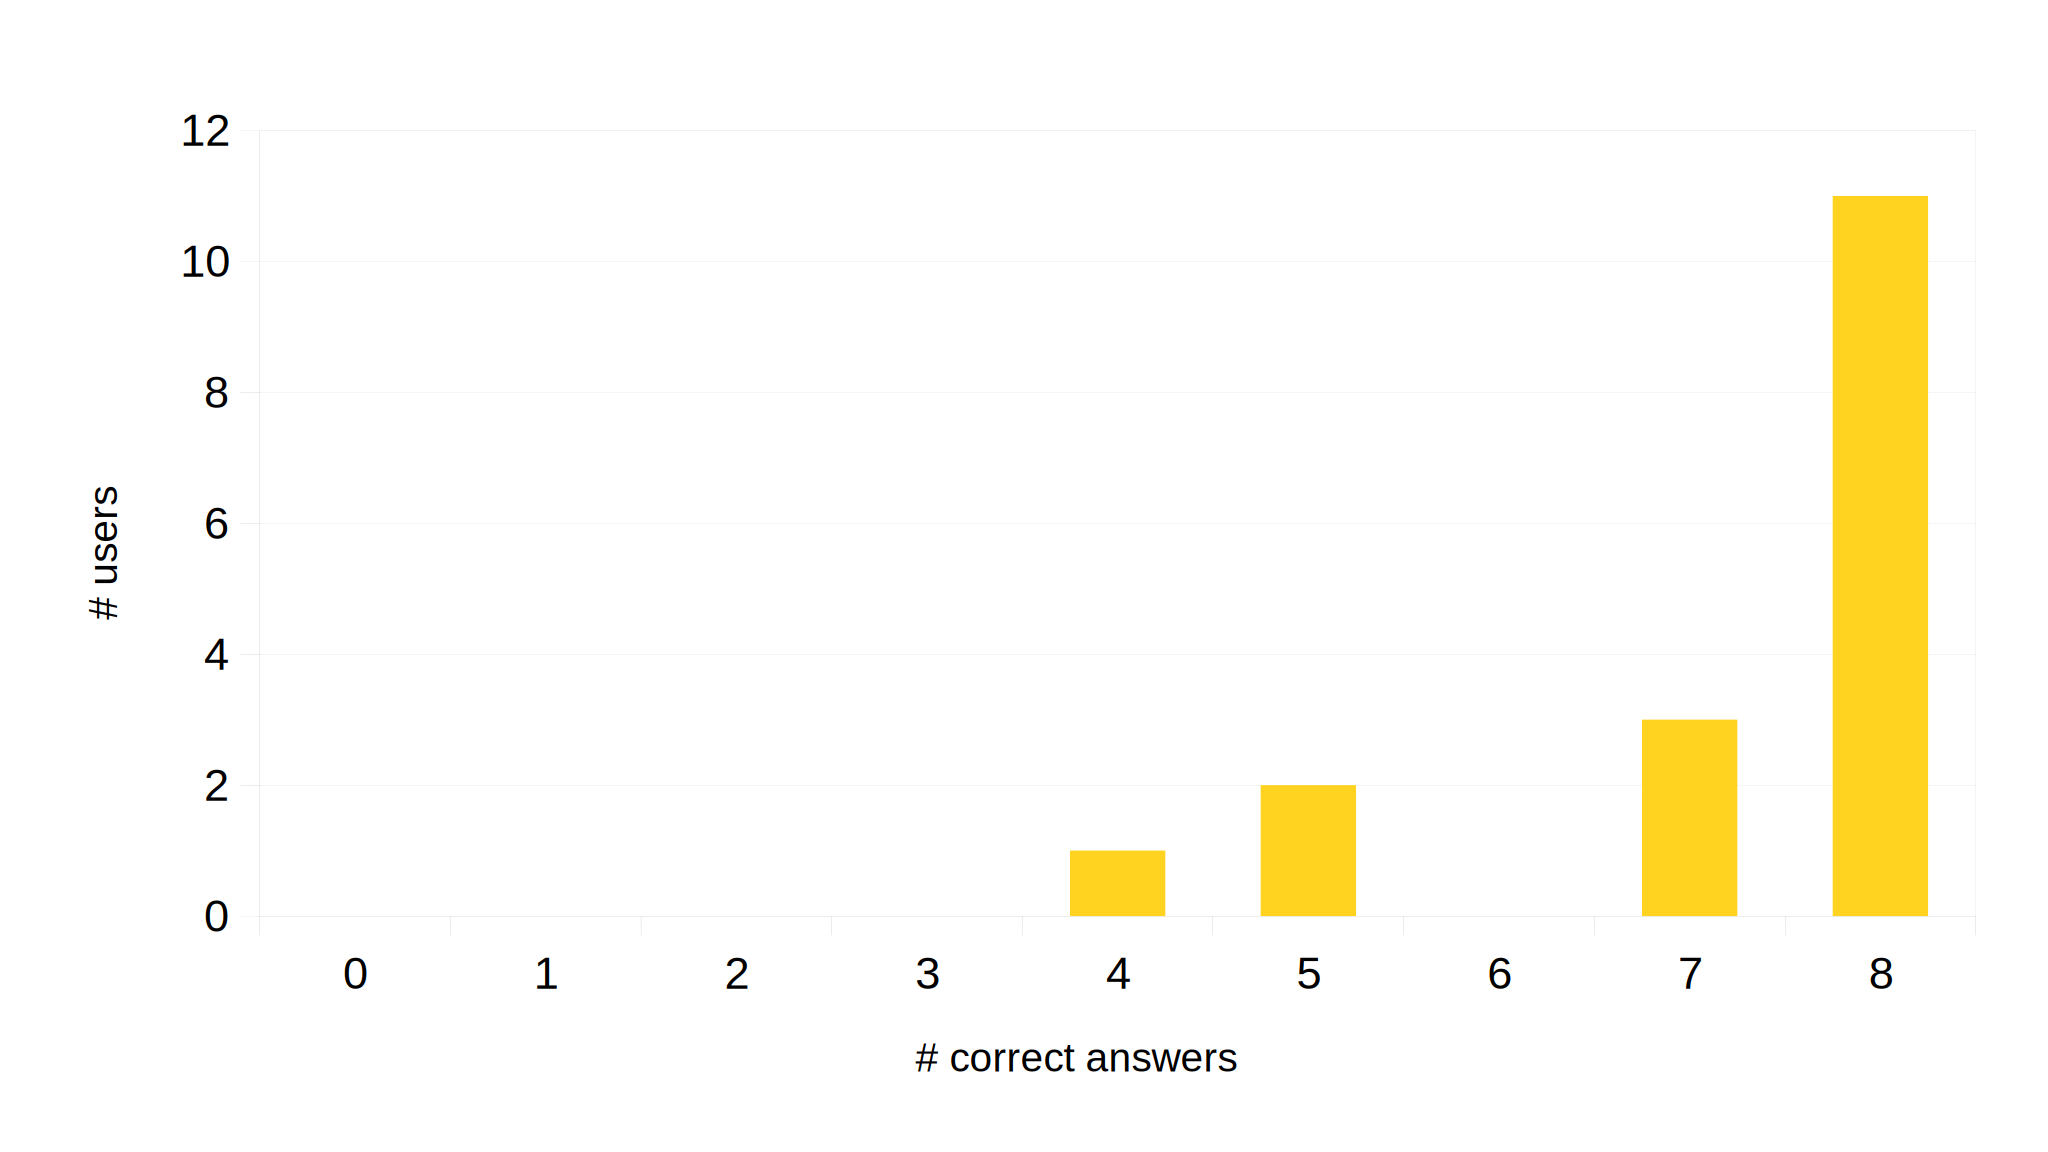
\includegraphics[width=0.45\textwidth]{hyp1anew.pdf}}
\subfigure[After (Repeated URLs)]{\label{fig:hyp1resultsarepeat}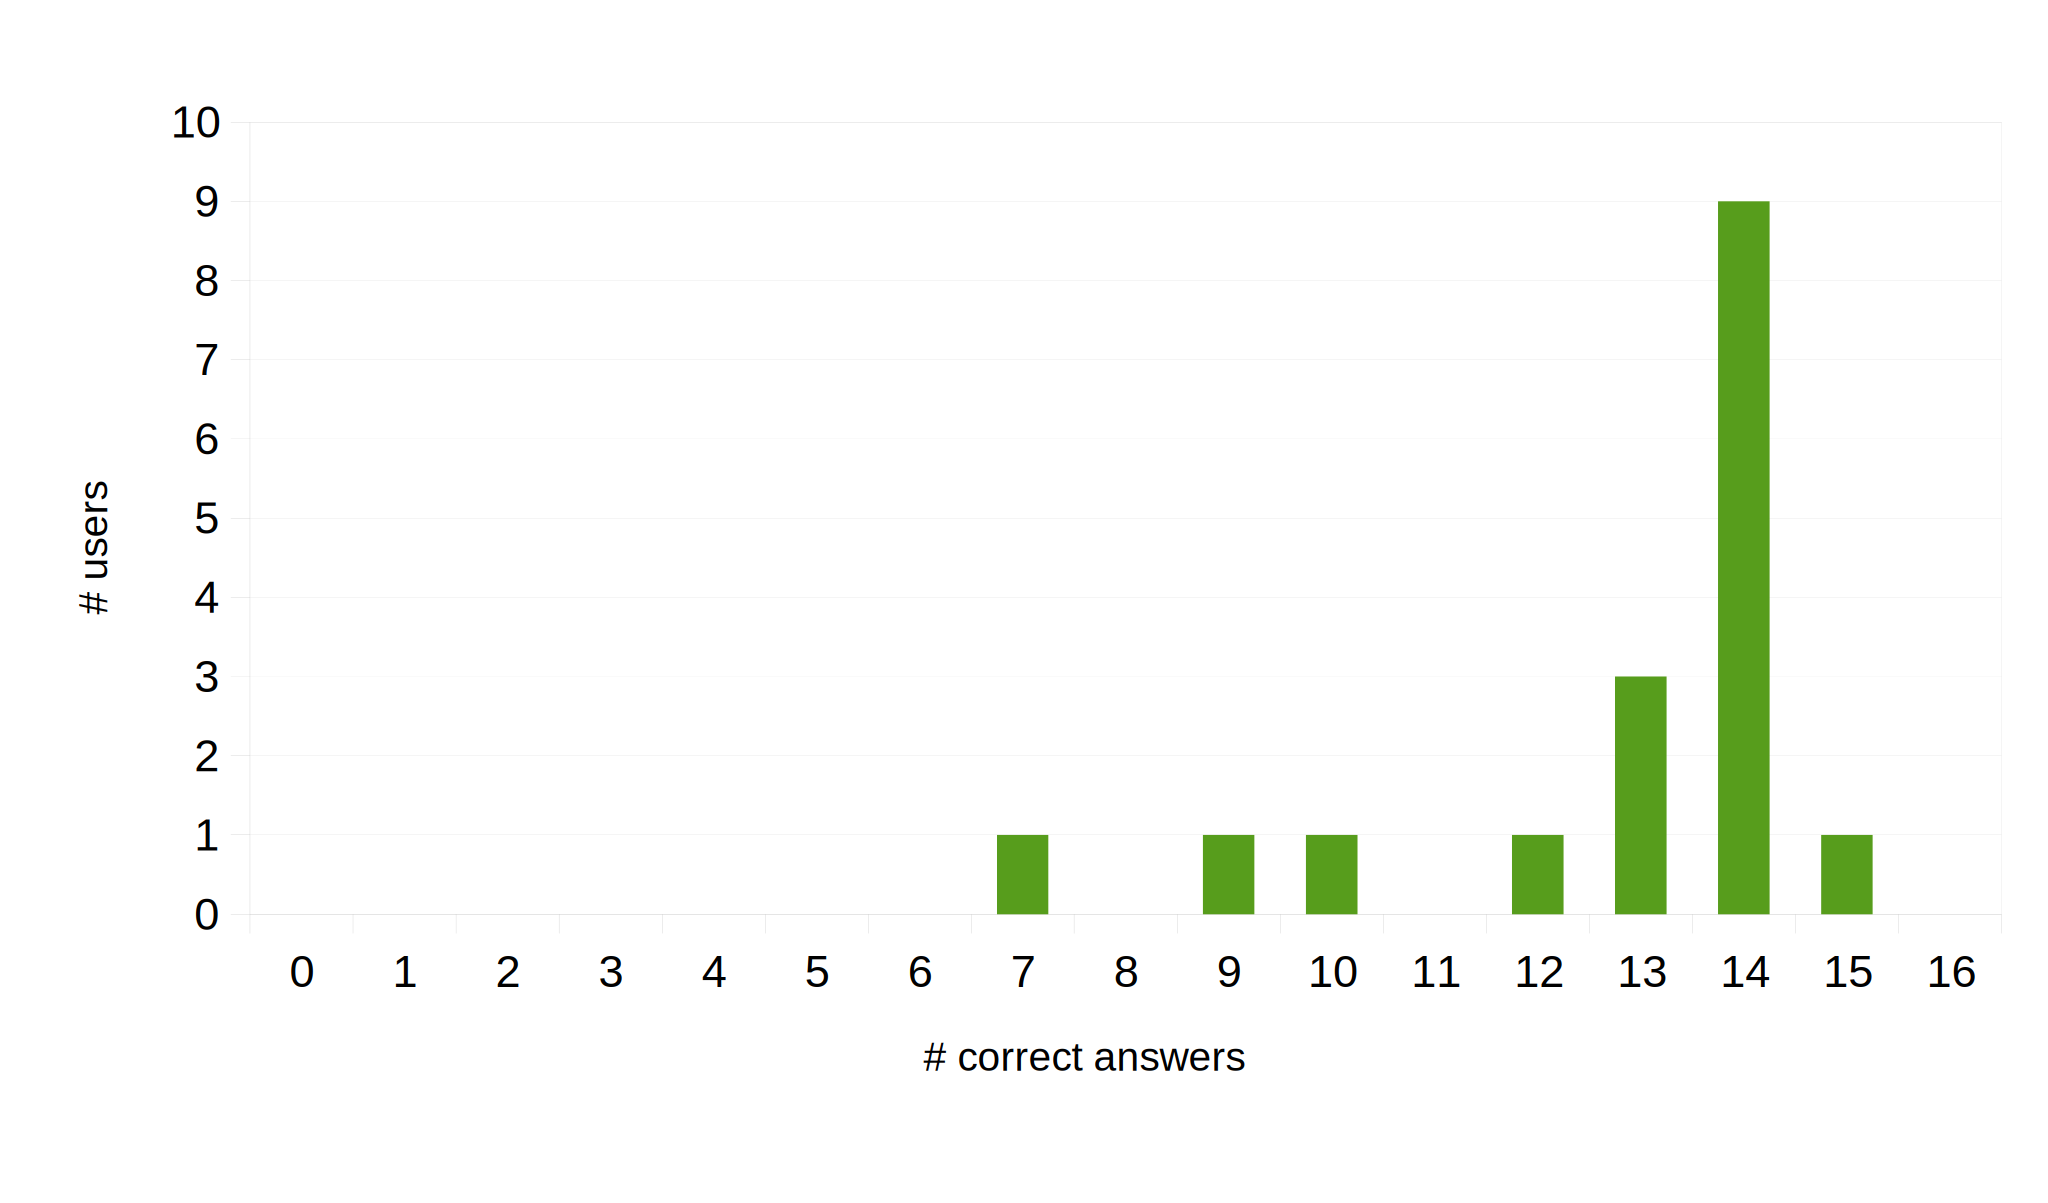
\includegraphics[width=0.45\textwidth]{hyp1arepeat.pdf}}
\caption{Correct Answers}
\label{fig:hyp1results}
\end{figure}

\begin{figure}
\centering
\subfigure[Before]{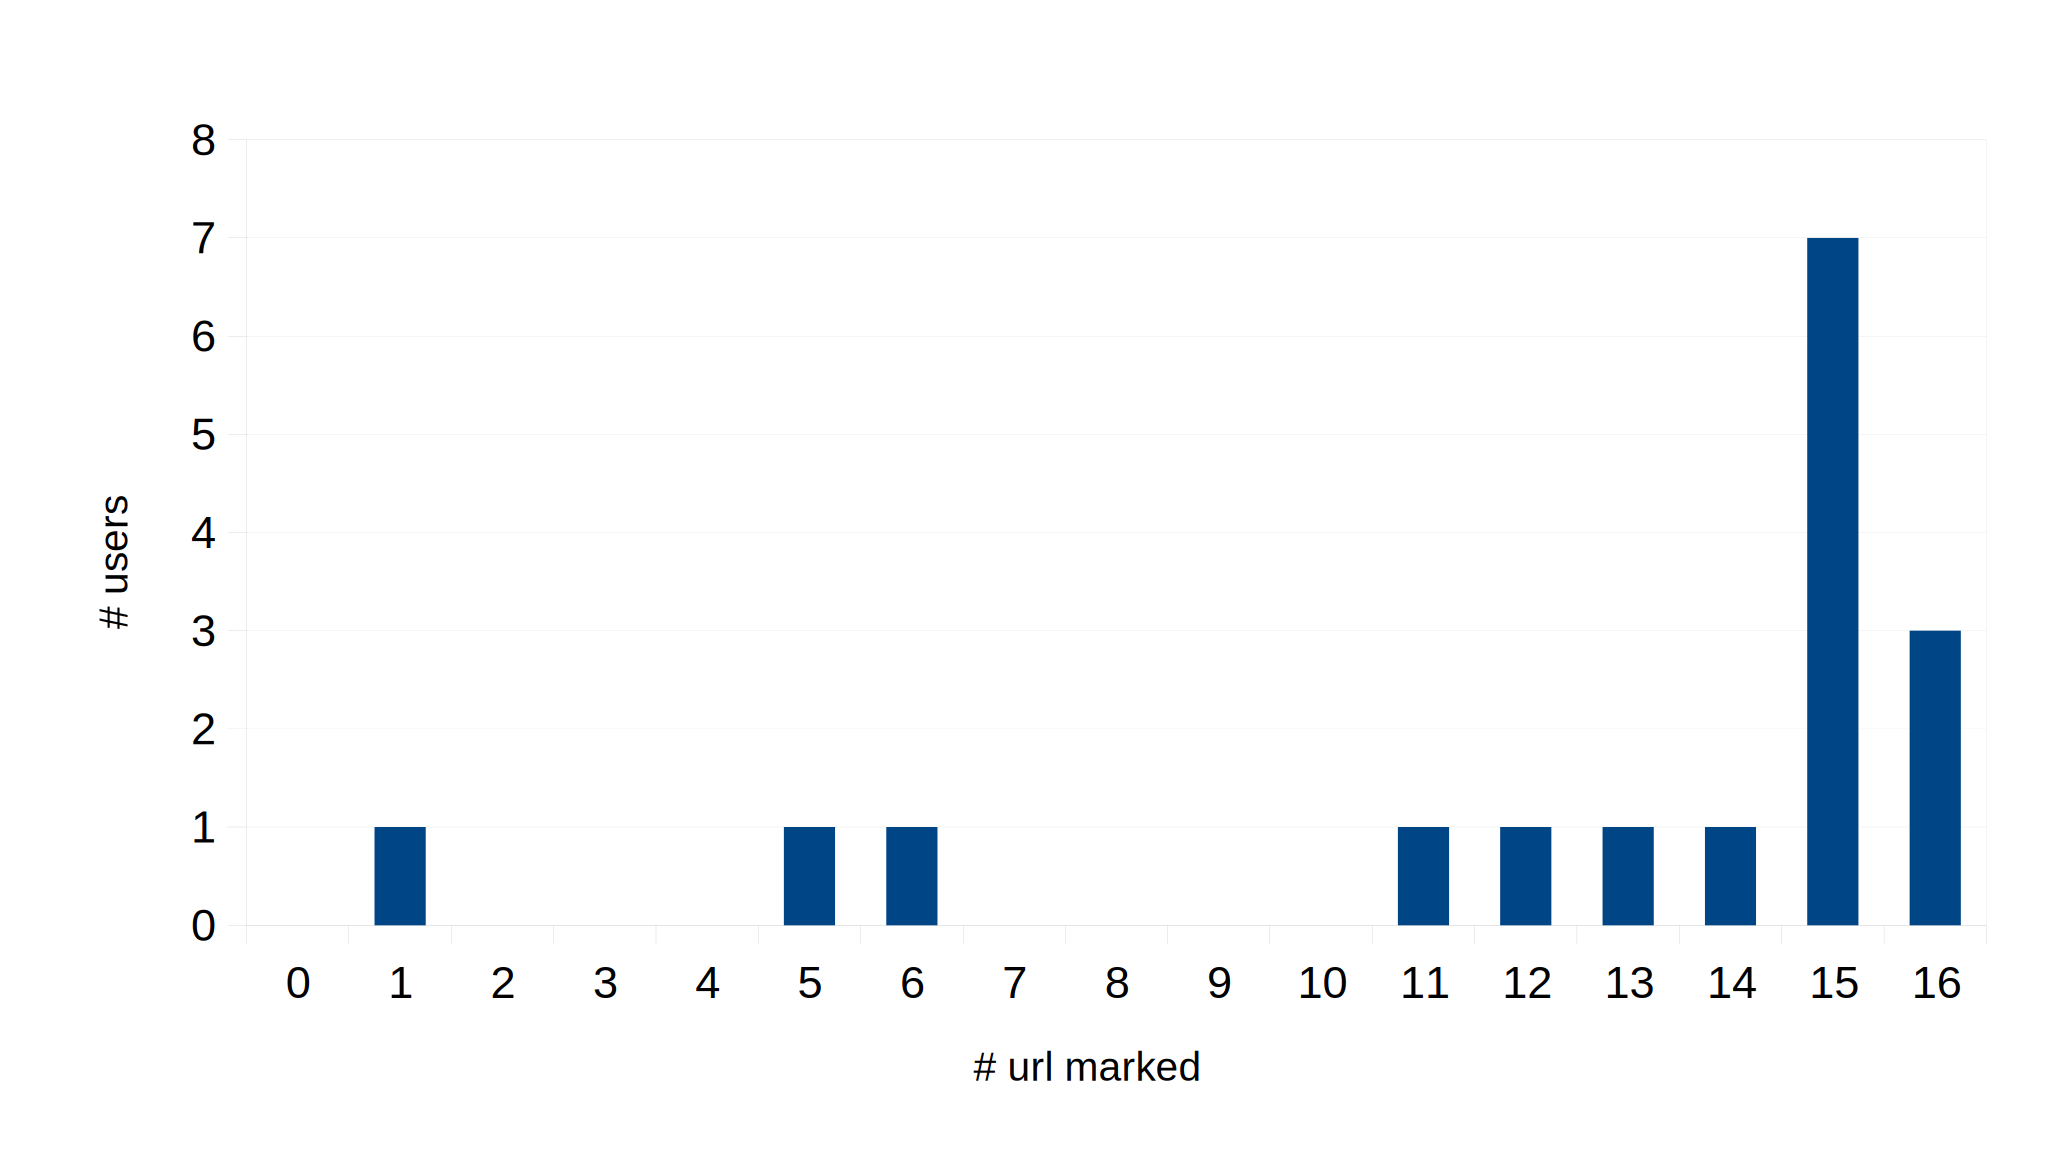
\includegraphics[width=0.45\textwidth]{hyp2b.pdf}}
\subfigure[After]{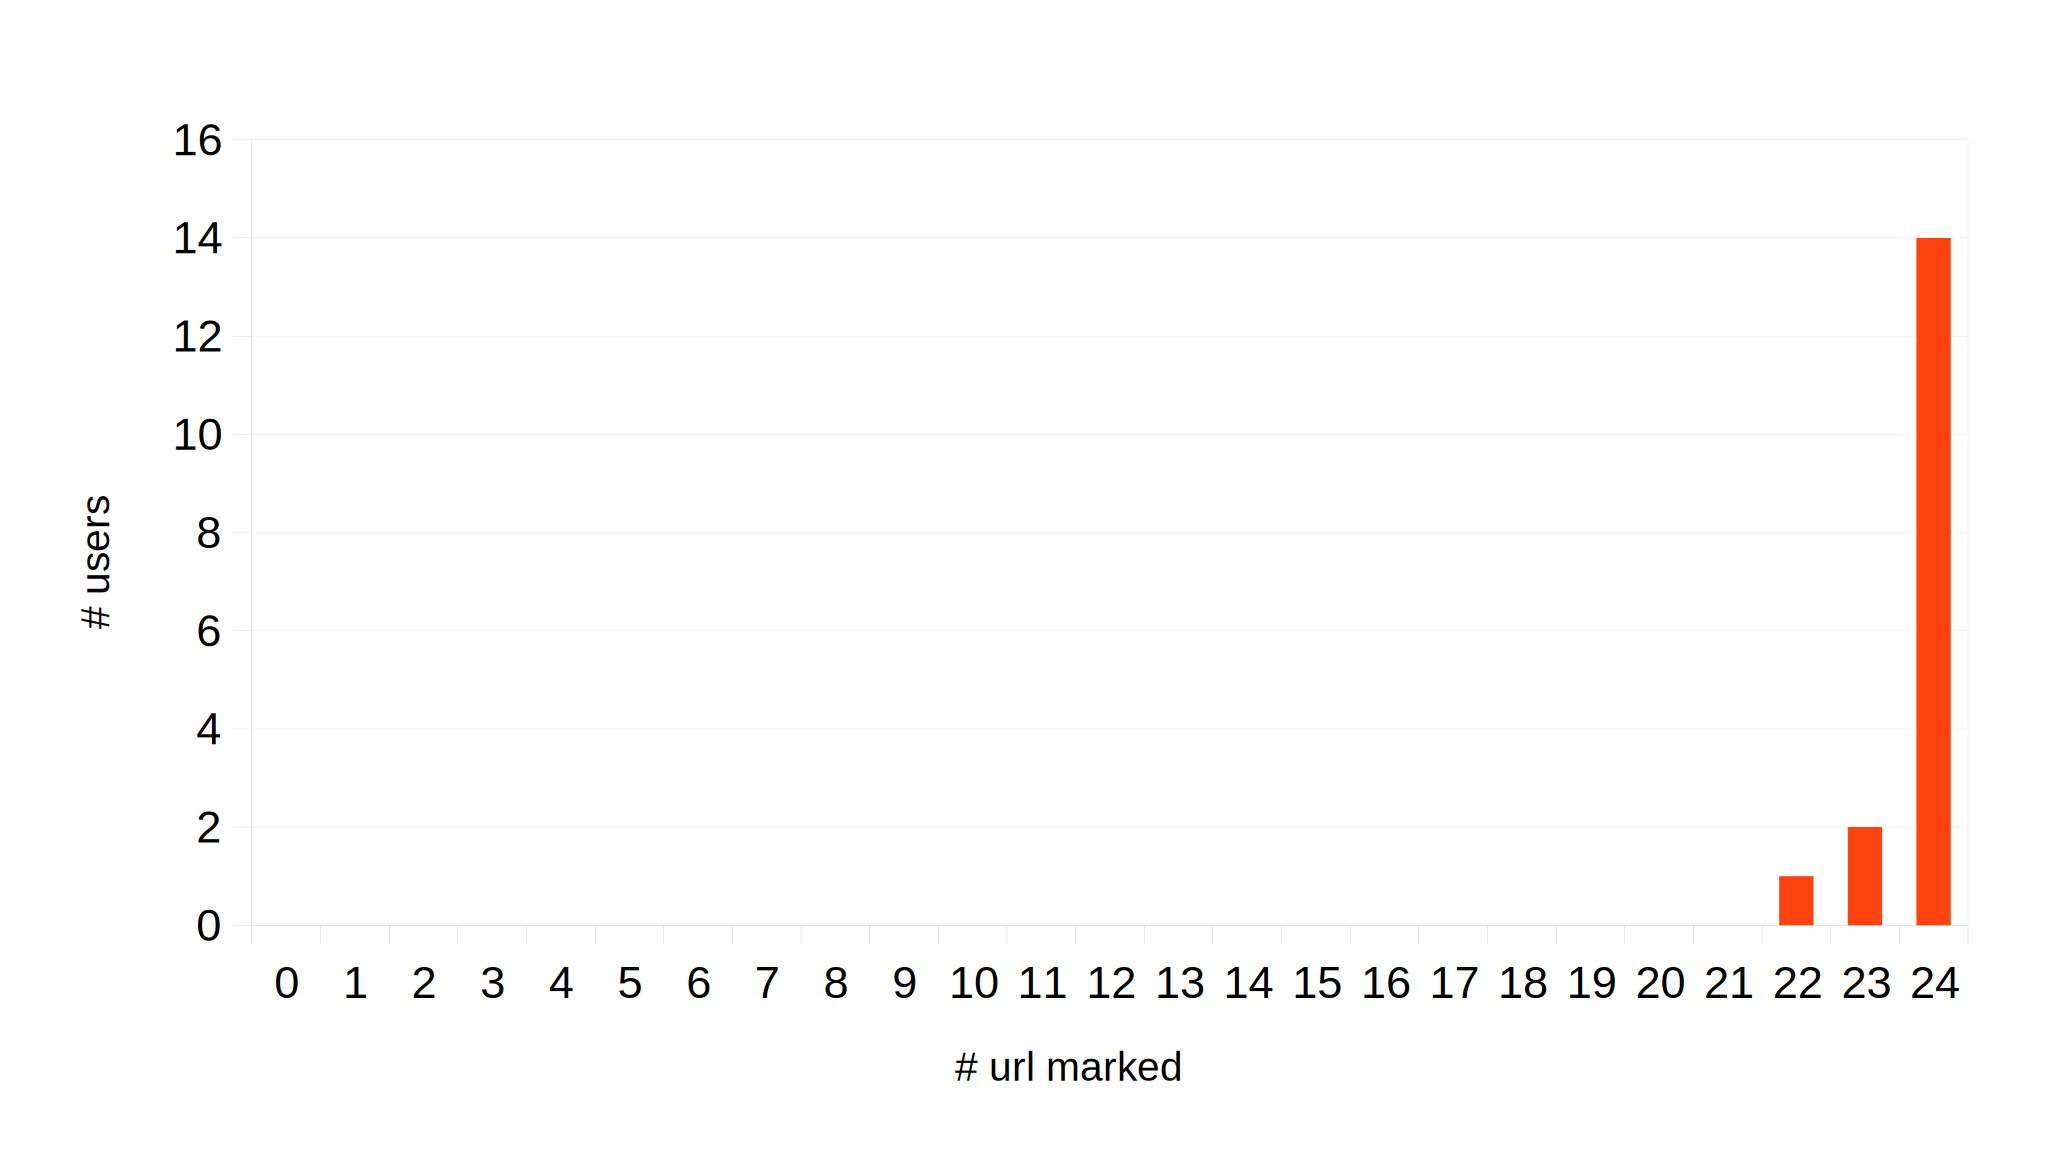
\includegraphics[width=0.45\textwidth]{hyp2a.pdf}}
\caption{URL marked}
\label{fig:hyp2results}
\end{figure}

\begin{figure}
\centering
\subfigure[Before]{\label{fig:domain_before}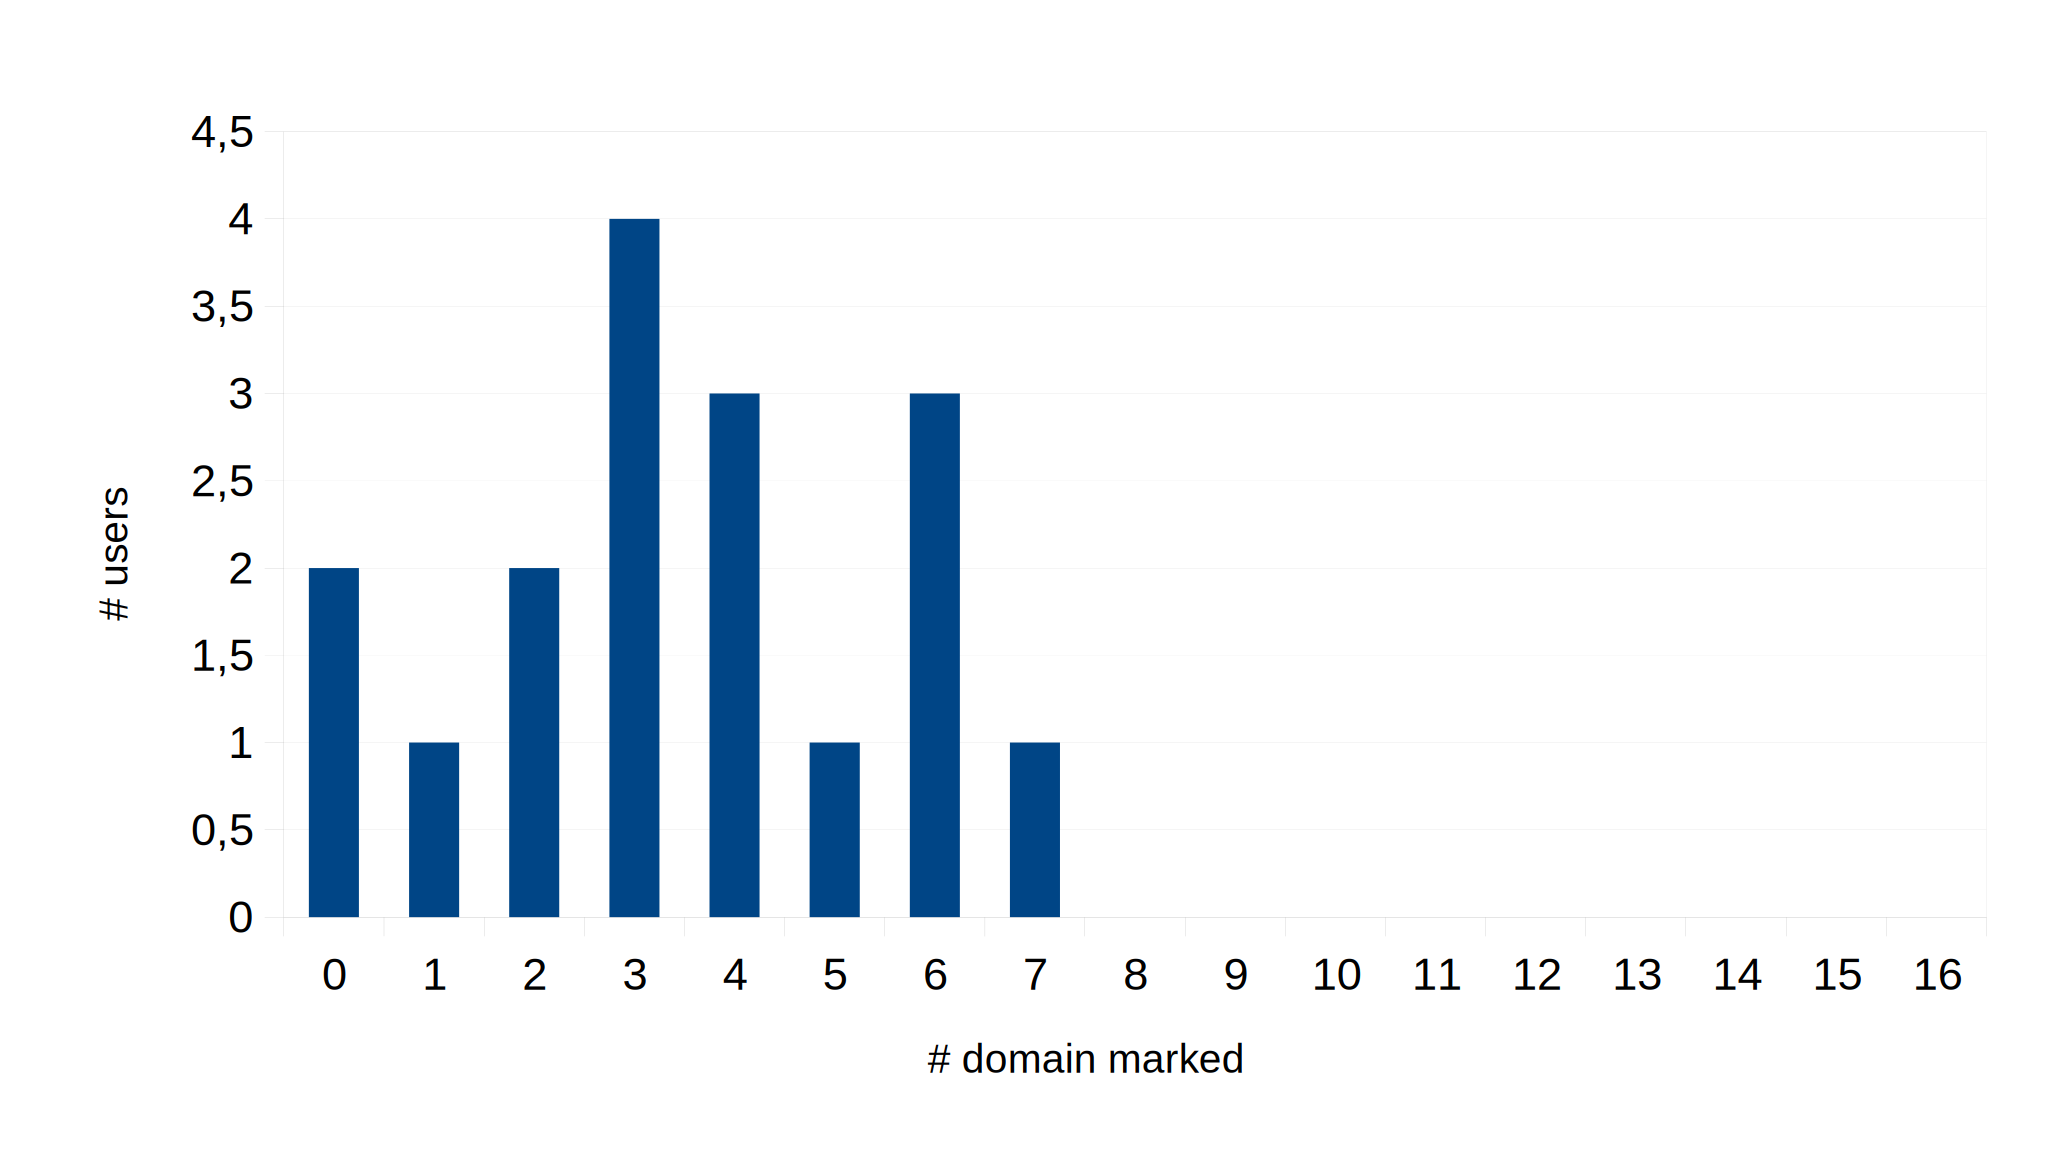
\includegraphics[width=0.45\textwidth]{hyp3b.pdf}}
\subfigure[After]{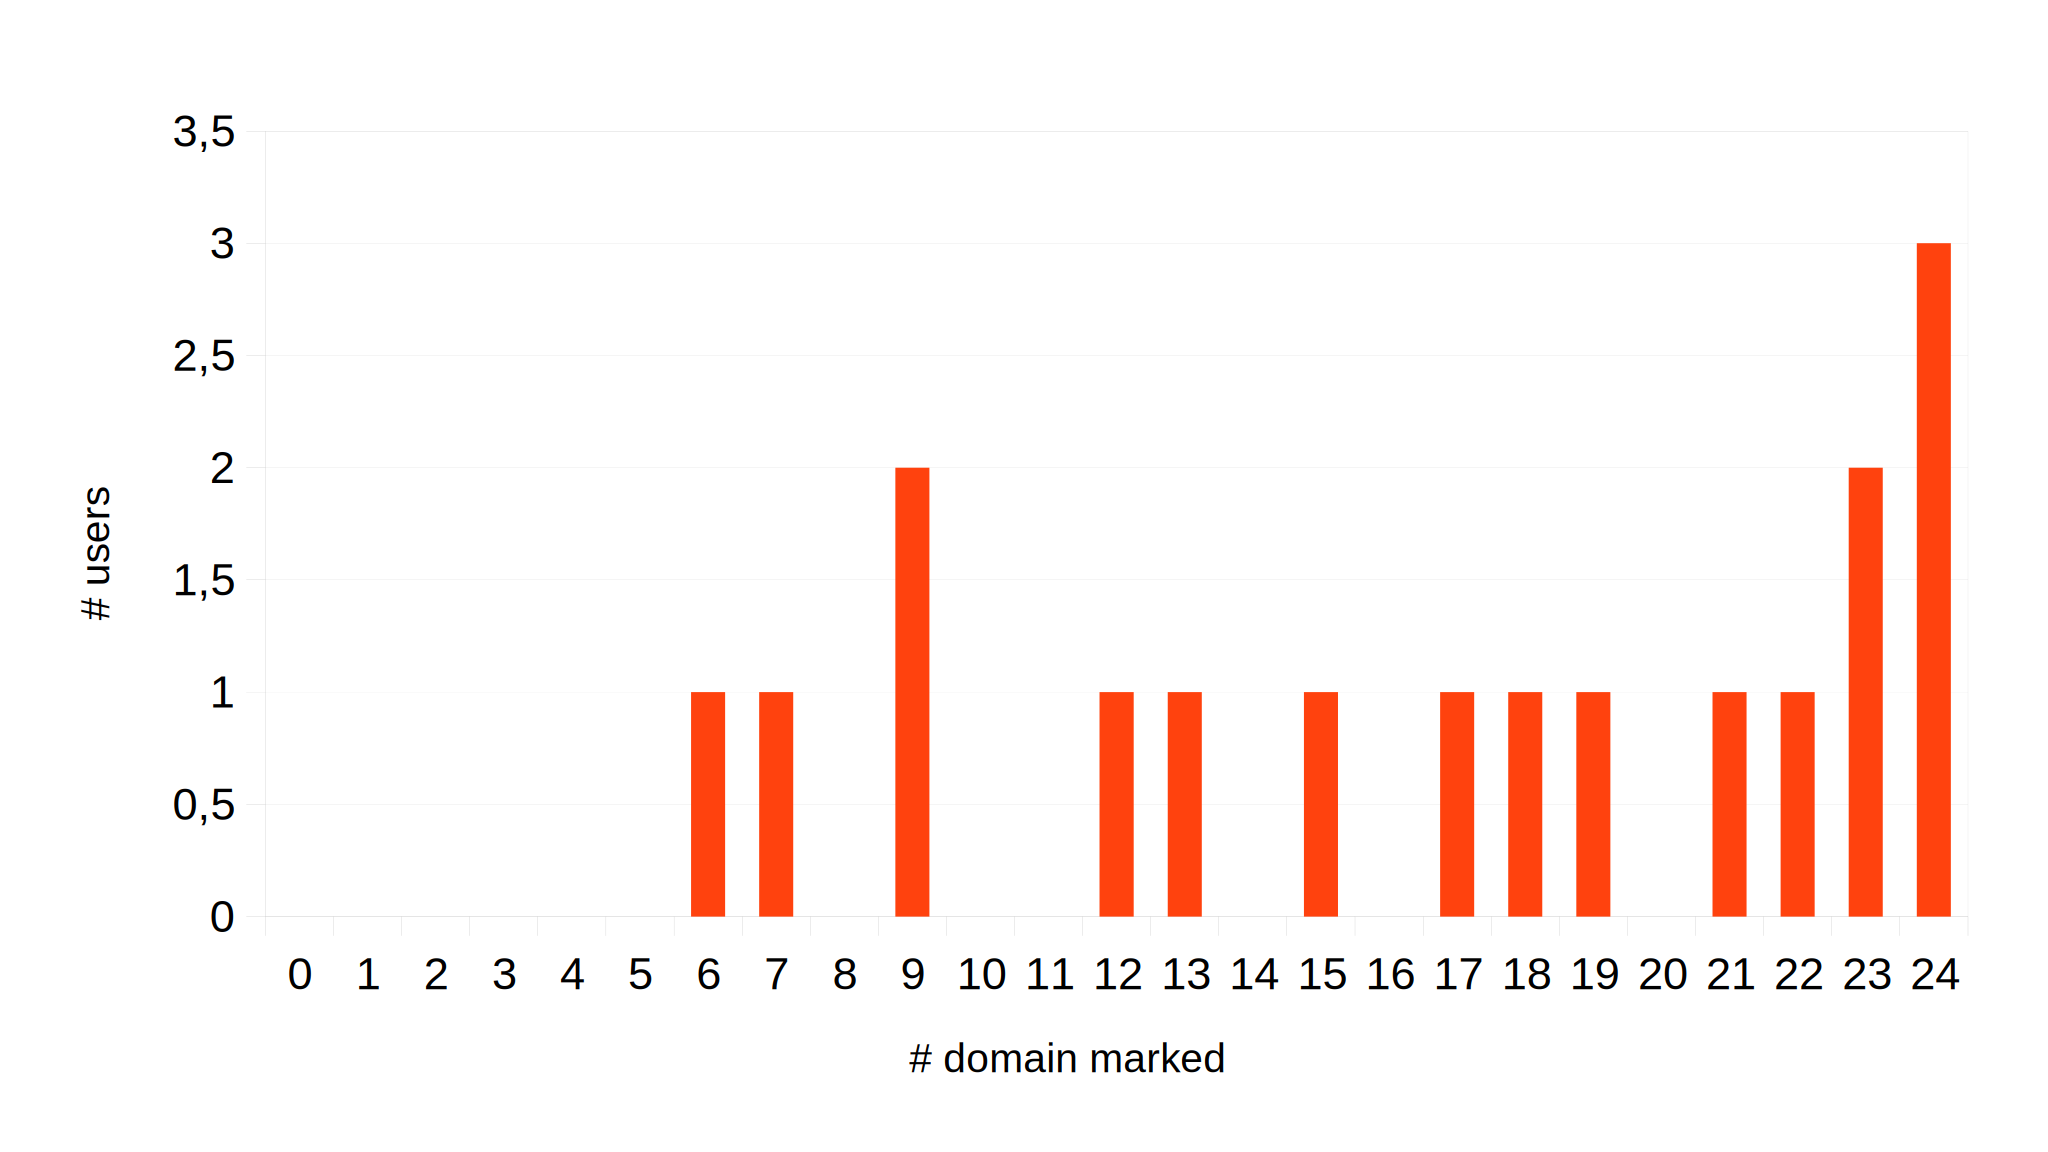
\includegraphics[width=0.45\textwidth]{hyp3a.pdf}}
\caption{Domain marked}
\label{fig:hyp3results}
\end{figure}

\begin{description}[leftmargin=0cm]
\item[Hypothesis 1:]
\autoref{fig:hyp1results} shows the results of our study according to hypothesis 1. One can clearly see that the majority of the users identified more URLs correctly after using the app than before. While most participants correctly identified 8 out of 16, i.e. 50\%, websites before they played the app, the majority gave correct answers to 22 out of 24 websites afterwards, i.e. 91.67\%. One could argue that this increase is based on the fact that the examples are mainly the same in the website-survey after, i.e. the reason for their better performance is based on learning effects. \autoref{fig:hyp1resultsanew} however shows that the user also gave correct answers to most of the new URLs. Therefore, we assume the learning effects are negligible.
In order to affirm our hypothesis we decided to apply the onesided Wilcoxon signed-rank test~\cite{wilcoxon1945individual} with our 16 samples from the website-survey before and the same 16 samples from the website-survey after.
Since we consider the learning effects negligible, we do not apply an alternative test against the 24 after URLs.
Our null hypothesis is $H_{0}: x_{1} >= x_{2}$ and the alternative hypothesis $H_{1}: x_{1} < x_{2}$, where x$_{1}$ represents the number of URLs which were correctly answered before playing the app and x$_{2}$ represents the number of URLs which were correctly identified after playing the app.
We computed the positive and negative rank-sums of $W_{+} = 141.5$ and $W_{-} = 11.5$.
The test statistic $w$ is the minimum of $W_{+}$ and $W_{-}$, hence $w = 11.5$.
As we chose $\alpha = 5\%$ as significance level and had 17 participants this results in a critical value of $41$.
As our test value $w = 11.5 < 41$ the null hypothesis can be rejected and thus the alternative $H_{1}$ is accepted.
Consequently, after playing the app the participants gave more correct answers than before.
We are aware that we cannot fully rule out the possibility that there might be kind of learning effect.
Yet, we are confident that these results cannot entirely be reduced to learning effects.
Therefore, we believe that our app helped users to make improved decisions about the legitimacy of URLs.
\item[Hypothesis 2:]
\autoref{fig:hyp2results} shows how many users marked the URL as their main source of decision.
Most of the users already based most of their decisions on the URL before.
Occasionally users marked the content or the padlock.
However only 3 Users (17.65\%) always marked the URL.
Afterwards we see that most users (82.35\%) always based the decision on the URL and only 3 Users made on or two mistakes.
Therefore we think that our app emphasized their believe in basing their decision on the URL.
We however think it is important to tell the user this to get uncertain or unknowing users to the same level as most of our participants.
Also our app empathizes the importance of the URL by putting the main focus on it.
We have decided against doing statistical test on this hypothesis.
We believe it will most likely be rejected because the change from before to after is not very high.
\item[Hypothesis 3:]
There is a general problem with one question in the websites-surveys.
In the before survey we were not able to clearly ask the user to mark the domain when it was the base of his decision because we would have then primed them towards looking at the URL or even at the domain.
This would have influenced the results of hypothesis 2.
Since we could not formulate this question clearly, a user might have marked the whole URL even if his decision was based only on a small part (for example, the domain) of the URL.
Consequently, we were not able to clearly identify what the users' main source of decision was in the before survey.
We were aware of this problem beforehand but saw no other option than formulating the question in such an open form.
Afterwards, the user knew that they were expected to mark the domain.
This can be interpreted as a change of question even if the literal question did not change.
Therefore, we cannot apply any statistical tests on this hypothesis.
Yet, we want to have a look at the results.
None of the users marked the domain in most cases beforehand, in particular, 7 domains out of 16 URLs where marked at most by only one user, cf. \autoref{fig:domain_before}.
\begin{figure}
\centering
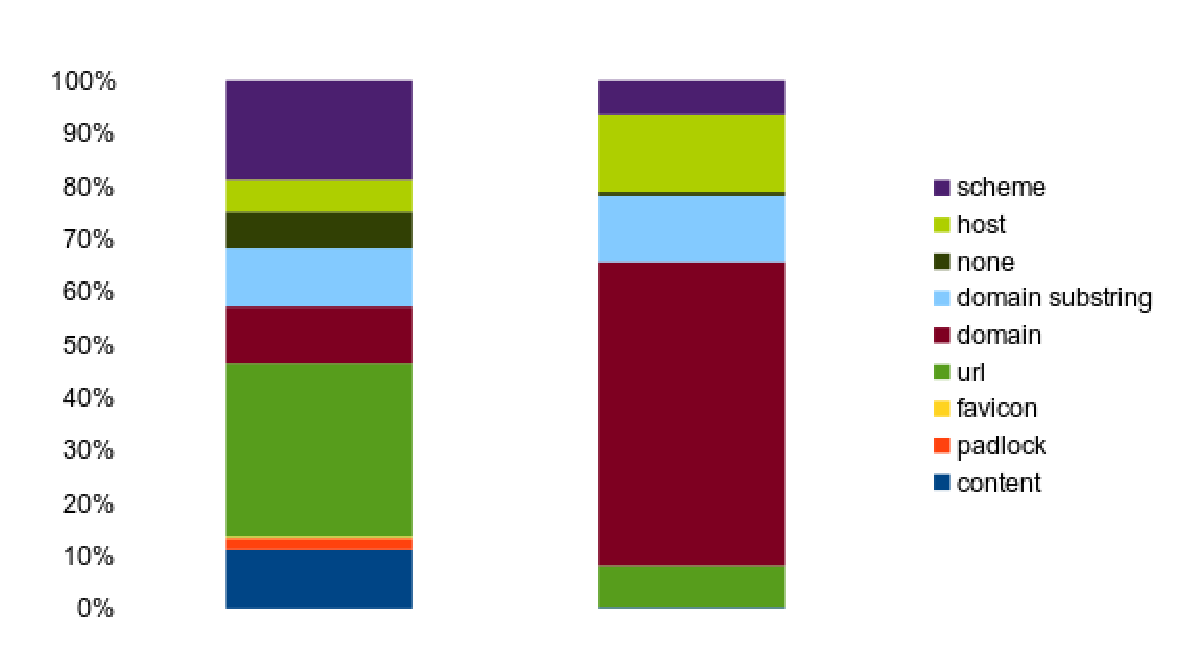
\includegraphics[width=0.65\textwidth]{markings.pdf}
\caption{Marked parts of the screenshot before and after}
\label{fig:markings}
\end{figure}

\begin{figure}
\centering
\includegraphics[width=0.65\textwidth]{legitimate_markings_after.pdf}
\caption{Marked URL parts of legitimate URLs}
\label{fig:legitimate_markings_after}
\end{figure}
\autoref{fig:markings} shows the distribution of the marked areas before and after playing our app. Obviously, afterwards most of the users marked the domain. However we are not able to compare that to the before values because of the changed question.
Another interesting observation is that quite a number of participants marked the complete host (instead of the domain) in case of legitimate URLs, cf.~\autoref{fig:legitimate_markings_after}. One explanation for this might be that we did not ask the user to mark the domain of legitimate URLs except in level 1.
\item[Hypothesis 4:]
According to the answers that the users gave in the After survey SUS section (\autoref{s:after_survey}) we calculated a SUS of 83.1. This is above 68 which means that we can consider our app above average usable.
\end{description}

%.........................................................................................................
\subsubsection{Further Study Outcomes}
%.........................................................................................................
\label{s:further_exploration}
Besides the results of our hypotheses the study yielded some further interesting outcomes.
This section further explores the results we obtained from our survey data and where not part of our hypotheses.
Afterwards, we summarize the participants' remarks to our app.

%.........................................................................................................
\paragraph{Further Data Exploration}
\begin{description}[leftmargin=0cm]
	\item[Correct and Reasoned Answers:] Hypothesis 1 only refers to giving a correct answer to the question whether a website is a phish or not.
	Our results show that users did not only give more correct answers after playing the app.
	In addition to their correct answer they reasoned their answer appriopriately (i.e. marked the domain).
	In the website-survey before 37.5\% of the URLs were answered and reasoned correctly.
	After playing the app 75\% of the URLs were correctly identified and reasoned. 
	Note, that reasoned means by our definition that the domain was marked in addition to giving a correct answer.
	However, a reasoning must not always rely on the domain itself. 
	As discussed in \autoref{s:hypanalysis}, for example, there were numerous participants who often marked the host of legitimate URLs.
	This is a correct reasoning for their decision, however by our definition it was not considered as such.
	Also, there were plenty of users who detected a phish and marked the attacked part instead (cf. \autoref{fig:m_attack_recognized}).
	By our definition this was also not accepted as correct reasoning.
	Hence, if we had expanded our definition of reasoning even more users would have correctly reasoned their decisions.
	However, there is the question whether expanding the accepted answers might also result in an increase of the correct answers and markings in the before survey.
	\item[User Opinions to App:] A part of our surveys tried to understand the users' opinions to our app.
	Section 3 of our survey-after (cf.~\autoref{s:after_survey}) contains the statements which the users had to assess with the aid of a Likert scale.
	Our worst, but still decent, score referred to whether the user was motivated by the spoofed e-mail to continue playing the app (average of 3.56) and whether the amount of texts was appropriate (3.53).
	We were beforehand aware that opinions of these two aspects might differ.
	This is also reflected by the individual answers.
	Many people strongly agreed with the statement that they were motivated and found the text amounts appropriate.
	However, there were obviously also people who disagreed with the statements.
	A reason for this might be, for instance, that they were already aware of the easiness of e-mail spoofing.
	All other statements were strongly agreed with in average.
	The text legibility of our app texts received an average score of 4.7.
	Our study participants in average strongly agreed (4.82) that our app helped them to identify phishing websites in future.
	%Yet, this requires a change in their behavior (checking the correct part of a URL) and retaining the obtained knowledge what we cannot check.
	Finally, the users intuitively understood our three lives scheme per level (4.411).
	Thus, the outcomes of the user opinions reveal that our app was well received by the participants regarding these questions.
	\item[Achieved Levels:] In average the participants reached level 7, which is higher than we had expected.
	We assume that some users started to roughly scan our texts for relevant information (for example, mainly looking at the examples) after they understood the importance of the domain.
	One user even played through the app in 30 minutes.
	In fact, this user has performed worse by the terms of our definition of correctness.
	The user had correctly identified 75\% of the URLs before playing the app.
	Afterwards, he only had a score of 54.17\%.
	The problem was that level 9 deals with the difference of HTTP and HTTPS websites and that we did not expect the users to achive a level higher than 8.
	Therefore, we did not consider HTTP and HTTPS in our assessment.
	Users were expected to decide whether a website is a phish or not disregarding the usage of HTTPS.
	The user who has achieved level 9 however was explained the difference of HTTP and HTTPS, additionally, he was asked to reject HTTP sites in general for this level.
	Hence, this user responded to the website-survey after respectively: the participant generally rejected HTTP sites whether they were phishing or not and thus the user performed worse afterwards by the terms of our definition of correct.
	All other users performed better after playing the app.
	\item[HTTPS and Padlock:] Our results show that some participants were aware that they should look for either HTTPS or a padlock before playing our app~\autoref{fig:markings}.
	For instance, one participant marked the scheme or the padlock as reason for his decision 11 out of 16 times in the website-survey before. 
	Another participant marked the scheme or the padlock of 8 examples.
	These participants trusted the padlock resp. HTTPS websites and distrusted HTTP.
	Consequently, they fell for phishing websites which make use of HTTPS in our survey and are likely to fall for such attacks in reality.
	Thus, the users who based their decisions on these indicators did not seem to be aware of the fact that the use of HTTPS does not necessarily mean that the website is trustworthy in general.
	In fact, there may be phishing websites using HTTPS.
	Therefore, we think it is important to introduce the level dealing with HTTPS earlier since we cannot assure that an app user of ours plays until level 9.
	This aspect should definitely be covered in future work in our opinion.
	
\end{description}

%.........................................................................................................
\paragraph{Remarks of Participants}
During playing the app, the participants had a slip of paper for notes they wanted to make considering the app.
In the following we outline the main results of these slips of paper.
Note that we did not ask the users to write down something specific. 
We merely asked them to write down what they thought, i.e. there might be more participants who agreed with some of these points below but just have not explicitly written it down.
In the following we consider the notes and suggestions of all participants. 
%TODO: Confidence of answers
\begin{description}[leftmargin=0cm]	
	\item[Scrolling of URL:] In addition to deciding whether a URL is a phish or not, the user has to face two more challenges. 
First, the font size gets increasingly smaller in higher levels, until it eventually is approximately the same size of the Android standard browser.
Second, the URL is displayed in a horizontal scrollbar so that the has to scroll the URL to the right in order to view the beginning of it, just like it is the case in browsers.
4 of our 19 participants found this disturbing and said it hindered them from analyzing the URL reasonably. 
This supports the importance of the introduction part 2 (access address bar) in the app.
The scrolling is present in order to simulate the behavior in the browser and it is important for a user to practice this.
We assume that the users would not have noted this in this extent in case they had completed introduction part 2, because then they would have understood why we do the URL scrolling during the exercises.
Yet, we think after a couple of levels the users should have understood that they have to scroll the URL, in the game as well as in the browser, so one might consider to eliminate it after some time. 
	\item[Unknown Services:] We have mentioned the problem of unknown services in \autoref{s:problems_with_URLs}.
As we were afraid there are in fact services which are not familiar to several users.
4 participants mentioned this problem.
Even if we tried to make use of the most popular services with the aid of Alexa's~\cite{alexa} ranking we cannot assure that all used URLs are known by all users.
One idea to approach this challenge might be to provide an question mark button in addition to the check mark (no phish) and cross mark (phish) buttons. 
When a player clicks on this button, he can be told whether the given URL is a phish or not and why.
From this action the user would neither profit nor would he lose any points or lives.
Yet, we do not think that this is a major issue, since the users got at least until level 4 and most of them achieved even higher levels.
We are confident that the app in its current state is already implicitly able to teach the users about the legitimacy of unknown services.
After facing unfamiliar URLs and making or not making mistakes they will eventually learn whether to trust a service or not.
	\item[Question to Data Entry:] 3 participants noted that the formulation of our website-survey question ``Would you enter your sensitive data into this website?'' was ambiguous.
Thus, there might have been participants who selected ``no'' even if they did not think it was a phishing website, but they would generally not enter their data into this specific website.
Originally, the website-surveys before and after asked the participants whether they thought a given website screenshot was a phishing website or not.
After our test iteration of our study, however, we decided to add some context to the question and had to make this trade-off with respect to the new question's ambiguity.
As we told the user that this study was particularly about phishing and that their task was to detect phishing websites in the website-surveys before and after, we believed that the ambiguity of this question would be negligible.
	\item[Explanations and Comprehensibility:]
4 participants stated on their slips of paper that they found the explanations of the app very good and easy to understand.
1 of these 4 participants, however, added that there is partially much text to read.
Another participant (not under those 4) noted that there is too much and long text in general.
	\item[Button Positioning:] The positioning of our app buttons during the game are as follows: 
The left bottom corner has a check mark which represents that the user thinks the displayed URL is not a phish.
The right bottom corner has a cross mark which means that the user thinks the displayed URL is a phish.
After clicking on either of these buttons in the write bottom corner another button appears (where the cross mark usually is) which either is the continue or the verify button (depending on whether the user has to select the Who-Section or not).
2 of our participants indicated that the positioning of the buttons in the right bottom corner are suboptimal.
The problem is that accidentally double clicking, for example, the continue button in the right corner results in rejecting the next URL even if the user might not have intended to.
Even if only 2 participants explicitly criticized this aspect we believe that this is a legitimate point.
In fact, the positioning of the two buttons continue and verify should be different from the one of the cross mark.
This is an aspect which should be targeted in future work. 
	\item[Repetition:]
Repetition is an important element of our app.
In every level introduction we briefly repeat the so far learned parts of a URL (with a graphic) and the different attacks the user has seen until this point.
We also make use of repetitions during the exercise rounds, every level contains at least one exercise from the previous level.
2 of our participants explicitly indicated that our repetitions made them feel more confident and safer.
	\item[External Links:]
In the main menu of our app we have a button ``More About Phishing'' which leads to a list of external links to various websites about phishing.
Some of these websites are in English.
2 participants indicated that they did not like it to be led to an English website and would have preferred to be forwarded to a German one.
This reveals that we cannot expect our audience to have knowledge of the English language.
Therefore, only German websites should be linked in the future.
Another idea to approach this might be to provide in-app additional information.
That is, instead of linking to external websites, the app itself could provide additional categorized information in German.
This would solve the problem with the language of websites and at the same time the additional information would fit to our app layout and design.
	\item[Amount of Examples:] Our app starts with a small sample of URLs users have to decide on.
In every level the sample size increases as the number of possible attacks increases.
Only 2 participants found that our sample size was too large.
This might have been the result of the fact that the users had to play the game for half an hour at a time.
We believe that the number of examples are reasonable, assumed that a user does finish the app at a stroke.
	\item[Further Suggestions:] In their notes some users made several suggestions which we found interesting.
These suggestions include, for example, more text highlighting of new teaching contents or the suitability of our app to be applied in schools.
In \autoref{s:future_work} we elaborate on aspects for further research in more detail.
\end{description}

\subsection{Limitations}
We decided to conduct a study which compares the users' performance before and after playing our educational app.
Our study design has some limitations we were not able to address for several reasons that we are going to discuss subsequently.

\begin{description}[leftmargin=0cm]
	\item[Behavior Change:] In our study the participants were not in their usual environment. 
	Therefore, they likely behaved differently during our study.
	An alternative approach would have been to distribute the app to several participants and ask them to play it remotely.
	However, this has two major downsides: First, the user would have been remote and thus we would have less control.
	Second, testing the before and after app skills would have been difficult to realize in order to ensure a homogenous process among all participants.
	\item[Increased Attention:] At the beginning of the study the participants were told that the study dealt with phishing.
	Additionally, for the website-survey before and after they were explicitly asked to indicate whether the websites were phishing or not.
	That is to say, the user automatically increased his attention towards answering these kinds of questions.
	Designing an in situ study, where the participant would have been in their usual environment and would have not known about their participation, was not considered because such a design is ethically and legally questionable. 
	\item[Knowledge Retention:] Our study design focuses on the present.
	Given certain time boundaries, it was not possible to study the long-term influences of our app by conducting the after app scenario repeatedly. 
	Consequently, knowledge retention is an aspect which is not considered by our study.
	\item[Bias:] For the recruitment we endeavored to ensure that our participants are not close friends of ours. 
	We rather seeked for friends of friends or even completely unknown persons~(cf. \autoref{s:participant_recruitment}).
	Certainly, the presence of a minor bias cannot be totally excluded.
\end{description}
Despite the limitations of our study we are confident that we got a good insight into the effectiveness of our app.

%===========================================
\subsection{Discussion}
%===========================================
Our hypotheses stated that our app can increase three major skills of the user.
First, we wanted to give the user the ability to detect phishing URLs.
This goal can be considered achieved as we could show that the increase is significant.
Even though there might be some learning effect we are confident that this increase is not mainly attributable to that.
The second and third hypotheses focused on the reasoning behind the user's decision.
We wanted to show that the user is aware of the fact that the content is no source of evidence against a phishing attack.
Our results suggest that most of the users already feel that the URL is important beforehand but some additionally consider the content.
Thus, the change in user response was not high enough to measure our hypothesis 2. 
The third hypothesis said that the users understand the structure of URLs better after playing our app.
As we discussed above, we had concerns about the design of the question that was intended to test this hypothesis.
The question has to be regarded as changed after playing the app.
Due to this, we could not consider the before-markings and could not argue on any findings about this hypothesis.

In addition to testing the hypotheses we got overall positive feedback from the users.
Most of them had the feeling they learned something from the app.
Some participants even contacted us asking about the release date of the app because they wanted to give it to their relatives.

Yet, there are still some improvements that should be considered when someone develops a next version of the app.
First of all, we think that the part talking about HTTP and HTTPS should be moved to an earlier level.
We saw many users that marked the scheme or the padlock in the URLs in the website-survey before.
This seems to be more important for the user than the URL itself because we had several users who fell for a phish and marked the scheme or padlock as reasoning.
As we cannot assume that users finish our app within one day, or even finish it at all, we think that it is important to clear that misunderstanding earlier.
The second improvement that a following developer should include is to restructure the app texts in such a way that the user can clearly identify repeating and new parts.
We think this aspect is not as important in real life compared to study situations because the app is not designed to be played a long time in a row.
This would increase the importance of the repetitions and make such a separation less important but this can be improved.
Last, it might be a good improvement to modify the app behavior depending on the user skill and performance.
This might prevent the user from getting bored.
This includes, for instance, vary feedback texts and icons depending on the user's performance as well as the degree of difficulty.
Another example is that the app could skip the proof part (identify Who-Section after detection of a phish) in case there is an indication that the user understood how to do it.
A simple form of that is already implemented.
The proof is shown up to a predefined level.
Yet, we think it is more reasonable to base the skipping and other possible extensions on the user performance. 

To conclude our findings despite some possibilities for improvement we can say that the app helped most of the users detect phishing URLs. This means we overall achieved the goal of the app.

	%*******************************************

\section{Conclusion, Recommendations and Future Work}
%*******************************************
\label{s:conclusion}

This chapter provides a short summary of what we achieved in the scope of this thesis and some further concluding remarks.
We also present a short list of recommendations regarding the design of security education games based on the lessons we have learned.
Finally, we have a short outlook on future work.
%===========================================
\subsection{Conclusion}
%===========================================
The objectives of this thesis were twofold.
First, we aimed at increasing users' security awareness so this may hopefully result in a change in their security-related behavior.
Second, we focused on the education of users with regard to the detection of phishing URLs. 
Our app is supposed train the user to achieve the required capability of correctly parsing URLs and thus identifying phishing websites.
This capability will hopefully help him to defend himself against phishing attacks.

To achieve these goals we developed an anti-phishing education quiz based game.
Our app targets the awareness increase by actively let the user spoof an e-mail and exemplifying him that a link does not necessarily lead to the target that it displays.
By letting the users practically experience this, we hope to increase the intensity of their learning experience (cf.~Principle~of~Intensity in \autoref{s:learning_principles}) resulting in a better and higher learning performance and motivation. We are aware that this part of the app might not be interesting and motivating for some users.
This is especially reflected by the answers to our question in the survey-after, where we ask whether this part motivated them to continue playing the app. 
The answers to this question are rather dispersed and thus result in an average value of 3.611 out of maximal 5 which would indicate that the user absolutely agrees.
Yet we think it is an important part of the app since there still seem to be users who are not aware of the facts that are taught in this part (the median is 4 out of 5).

After motivating the user with practical examples and increasing his security awareness the actual game starts.
The game itself consists of levels with introductory parts followed by practical exercises the user has to solve in order to show he has understood the learning content.
Initially, in introduction 2 (access address bar and view complete URL) and level 1 (URL basics and domain identificationzich), basic knowledge is covered which is required for the succeeding levels and especially for the detection of phishing URLs on the smartphone in general.
In particular, introduction 2 might be not challenging enough for some users as they might be already well-skilled regarding smartphone functionalities.
Yet, this introduction and exercise is indispensable as there might be users who do not know this.

In levels 2-9 the user is introduced to various attacks a phisher might apply.
These attacks get increasingly sophisticated and harder to detect with higher levels.
Finally, in level 10 the user gets further final remarks, such as the discussion about legitimate URLs which might appear fraudulent but in fact are not, or some input to extended validation certificates and a link for further information.
We generally aimed at using introductory texts that are simple and easy to comprehend.
We think we achieved this goal as our participants agreed to this (cf.~\autoref{s:further_exploration}) and the legibility index further confirms it~(cf.~\autoref{s:legibility_index}).

The study outcomes suggest that there is a possitive effect which is likely resulting from our app.
Our participants clearly gave more correct answers (is a given website a phish or not) after playing the app compared to before.
Before playing the app most users identified 50\% of the 16 websites correctly.
After playing the app the majority of the participants gave correct answers to 91.67\% of the 24 websites.
We assume the learning effects are negligible as the distribution of the correctly answered new URLs is almost identical to the old one (cf. \autoref{fig:hyp1resultsanew} and \autoref{fig:hyp1resultsarepeat}).

The results of our second hypothesis exposed that the users already knew it was important to look at the URL before playing the app.
Yet, they obviously did not know where exactly too look at as their result in correct identifcations show.
Even if there were many participants who looked at the URL already before playing the app there is a significant difference in the following aspect:
Before playing the app only 3 (17.65\%) users always marked the URL.
In contrast to that, after playing the app most, i.e. 14 of 16 users (82.35\%), always marked the URL.
Evidently, our app was able to emphasize their believe in basing their decision on the URL rather than the content or anything else.

The measurement of our third hypothesis was questionable.
The problem is the following: after playing the app we virtually changed the question when asking the user to mark the area of their primary reason for their decision.
With the app we primed them to mark the domain clearly.
Before using the app the users might have meant the domain, but just did not clearly mark it because they did not know what exactly they were expected to mark.
Still, we analyzed our results on this question and found out that more people base their decision on the domain after playing the app.

All in all, we can say that our app has a positive effect on users and that it helps them to better identify phishing URLs.
However, the question to ask here is will this app actually help users change their behavior in the Internet and make them look at the URL even if it is only occasionally.
This is an aspect, which we were not able to address within the scope of this work
Finally, the study conducted cannot show how the users, for example, retain the lessons learned from our app.
Such considerations remain open for future work.

%===========================================
\subsection{Recommendations for Security Education Games}
%===========================================
Technical solutions are not 100\% accurate at detecting phishing attacks.
The education and training of users offers a complementary approach to these systems.
Based on our gained experience, we present design principles that we recommend to consider when designing a security education game:

\begin{description}[leftmargin=0cm]
	\item[Principles of Learning:] Since education games do not primarily aim at entertaining the user, but simultanously at educating him, it is important to take the priciniples of learning into account.
These principles state under which conditions learning performance is increased~(cf.~\autoref{s:learning_principles}).
We consider it especially important to rely on the principle of exercise, which states that training, repetition and feedback is crucial for good learning performance.
	\item[Game Techniques:]  If the education is supposed to follow with the aid of a game it is relevant to regard essential game techniques~(cf.~\autoref{s:game_techniques}).
In fact, game techniques are closely connected to learning principles.
They provide in-depth elaboration on how basic learning principles are achieved with games.
	\item[Simple and Short Text:] Education implies that some sort of text is present in some way.
The users to be educated may come from different fields.
While some users might be more skilled and might be able to handle complex texts on security-related topics others would probably get discouraged by such.
Skilled users are likely capable of acquiring knowledge on security topics without problems.
Security education should mainly address those users who are overwhelmed by such texts and information.
For these users it is important to provide simple texts which are easy to follow and not too long.
The longer texts are the more likely it is that the users will skip text parts which might be important or even stop reading it.
\item[Precise Phrasing:] The texts should be formulated precisely. 
If a text is not precise this might lead to misinterpretations and thus to mistakes. 
One should take care that there is as less room left for misinterpretation as possible.
\item[General Validity:] There is a range of potential learning content which might be important to communicate to the users.
Yet, there is the problem of general validity.
It is important to consider that, for example, aspects that apply to system A, for example an Android device, do not apply to system B, for example another version of the same Android device.
Therefore, in some cases it might not be easy to transfer knowledge about A to B (for example the browser functionality).
For this reason it is relevant to consider whether one wants to educate the users about aspects which are generally valid among several systems or whether the education focuses on specific systems which ultimately would result in restricting the target audience to those who use that specific system.
\end{description}


%===========================================
\subsection{Future Work}
%===========================================
\label{s:future_work}
This section deals with a prospect on future work for our Anti-Phishing Education App.
 In particular, we present ideas that might be beneficial and which we were not able to address and realize due to time and resource limitations.

\begin{description}[leftmargin=0cm]
	\item[Comparative Study:] A comparative study might be interesting, as the authors of Anti-Phishing Phil~\cite{sheng2007antiphishingphil} did it.
	They conducted a study with three different conditions,  a group that consulted general tutorials from the Internet, a  group who learnt from tutorials based on Anti-Phishing Phil and another group who played Anti-Phishing Phil itself.
	An interesting comparison to consider might be our app with Anti-Phishing Phil or any other anti-phishing app and general tutorials.
	\item[Study on Retention:] For time reasons knowledge retention is an aspect we could not address in our study.
	Yet, we think it is important to consider this in future work.
	The question to ask here is how well users retain the knowledge they obtain from our app compared to other sources, for instance.
	\item[Embedded Training:] In \autoref{s:related_work} we argued that exploiting the teachable moment might result in good motivation for a user to do something about his lack of knowledge regarding phishing and possibly result in better retention.
	Yet, a drawback of embedded training is that its landing pages are not able to provide detailed and extensive information on the topic since users would be discouraged and leave the page.
	Providing detailed and extensive information can be addressed by a game playfully.
	Therefore, an idea is to combine embedded learning with an educational game.
	Here the user would be forwarded to the landing page with the most important information in case he falls for a simulated phishing attack.
	On this page the user can be provided with the most important information and a link to an educational app, for example ours, where he can optionally get more detailed information.
	With the game the knowledge can be obtained step by step by playing the game.
However, there remains the problem of raised legal issues.
	\item[Malicious Downloads:] With our app we did not target the possibility of downloading malicious software when a user clicks on such a link.
	However, we think this is an aspect which should also be targeted in future work since malicious software can also cause harm.
	For example, the user could be told at some point that he should never open downloaded files he did not intend to download.
	Instead he should immediately delete them.
	\item[Certificate Validation:] We do not address the validation of certificates with our app. We also do not tell the user, for example, that he should at least not do banking in case a certificate is broken.
	Such general suggestions might also be considered for future work.
	\item[Data Economy:] Another relevant aspect we did not cover in our app is data economy.
	We tell the user to type in their data only into websites they are sure about their legitimacy.
	However, we do not tell the user to think about the specific data they are asked to enter.
	Users should re-think whether the required information is actually needed.
	This should also be trained by for example asking the user ``A lottery site is asking for your data. Which data would you provide?''. As this approach would require a complete different UI this type of learning content remains for future work.
	\item[Consequences:] Initially, our idea was to display the consequences for falling to a specific phishing URL (matching a certain website category). For time reasons, we had to delay this for future work.
	We still think that this kind of information is relevant for the user as it illustrates him on which websites he should especially take care, for example, on banking websites.
	\item[Increase Immersion:] Immersion is an important game element (cf. \autoref{s:game_techniques}).
	We believe our app has space for more immersion. 
	For example, an appealing story around our quiz game could be added in order to mesmerize the user.
	\item[Increase Effect:] In \autoref{s:learning_principles} we have introduced the Principle of Effect, specifically, the law of positive feelings. 
	We believe the user's positive feelings can be increased by providing more variable feedback, instead of saying the same sentence for the same outcomes.
	For example, the praises and compliments when a user does well could vary depending on the degree of difficulty.
	Also, the final screens for finishing a level can vary.
	\item[Top-Level Domain Attacks:] It might be reasonable to explicitly tell the user, that he should not only look whether the second-level domain is exactly as he expects but also the top-level domain. The app only implicitly states to look at the top- and second-level domain together.
We recognized that users might misinterpret this (problem of precision).
Therefore, this addition should be realized for future versions.
	\item[Performance Dependent App Behavior:] Currently the app is quite static.
More dynamic behavior could be added in future versions.
For example, the part where the user has to show the domain in case he found a phish might get tedious after some time.
To approach this problem the app could stop asking for the domain after the user identified the domain correctly 10 times in a row, for example.
After this point the app could occasionally ask the user to identify the domain and depending on his performance re-introduce it.
\end{description}

 




2 participants stated that the attacks in level 2 are not very challenging and very obvious.
Phishing URLs are of the following kind in this level: ``http://www.ebay.de.phisher.com/login''.
We had done this intentionally, however maybe the app could in fact start with for example nonsense attacks or just reduce the number of samples in this level.

Also some users suggested us to visually distinct new learning content from repetition so overflying the information part becomes easier. 
We had already tried that by displaying a warning sign every time a new attack was introduced.
However, after this sign there still was some repetition occasionally.
Therefore, the emphasis of new and relevant learning content in the lesson parts should be improved in future work.

Another participant noted that the repeating sentences ``Very good. You are now a bit safer'', for example, when the user correctly identified a phish, were kind of repetitive and not motivating enough. This is ultimately related to our issue with the Law~of~Effect in \autoref{s:learning_principles}.
There we stated that the texts and icons of the app should vary according to the user's performance and the degree of difficulty in order to achieve higher and better positive feelings.
This is an additional point which is worth to consider for future work.

A participant would have wished more ``feedback'' on his progress in general. 
He missed statistics, highscores or other forms of long-term feedback.
As we mentioned in \autoref{s:learning_principles} and \autoref{s:game_techniques} feedback is essential for learning as well as games.
For this reason, this aspect is something which should be enhanced in future.

A further interesting point is that one of our participants noted that he thought our app was appropriate for schools.
In fact, this appears to be a good and important point.
People might not want to learn about phishing by their own choice, especially pupils would probably not think about that.
However, if computer security is a part of the education plan and if pupils have to learn something about, for example, phishing by playing the app, a far larger audience can be reached and educated on this topic.

Finally, one user indicated that the design of our start menu could be more appealing.
This is a justified criticism.
In fact, we did not put our focus in design aspects.
To make the app's outer appearance more appealing design aspects could be considered for future work.


	\begin{appendix}
	\section{E-Mail Template of the Awareness Part}
\label{a:mail}
\lstset{language=html}
\begin{lstlisting}
<html>
  <head>
    <title>Anti Phishing Education</title>
  </head>
  <body>
    <p>Dies ist eine automatisch generierte E-Mail im Rahmen einer Anti-Phishing Education App. Falls diese nicht angefordert wurde, bitte ignorieren.</p>
    <p>Ansonsten geht es hier weiter:</p>
    <p>Wie du im Absender siehst, hast du dir gerade selbst eine E-Mail mit gefälschtem Absender geschickt. Hier ist außerdem dein Freitext:</p>
    <p>{$usermessage}</p>
    <p>Für einen Angreifer ist es ebenso einfach automatisierte E-Mails mit gefälschtem Absender und Inhalt zu verschicken. Meist enthalten diese einen Link zu einer Webseite, genau wie diese E-Mail.</p>
    <p>Um mit der App fortzufahren, klicke auf den folgenden Link.</p>
    <p><a href="http://pages.no-phish.de/maillink.php">http://www.google.com</a></p>
    <p>Viele Grüße,</p>
    <p>Dein NoPhish Team</p>
  </body>
</html>
\end{lstlisting}

%===========================================
\section{URL Generation Process}
\label{s:url_generation}
%===========================================
When playing the app (level 2-9) the user has to categorize a given URL as a phish or valid URL.
We decided against a fixed set of examples for the URLs because depending on the set size it might happen that a user keeps being confronted with the same URLs.
We believe it is essential for the user to be faced with as many different URL examples as possible.
Therefore, we decided to generate the URLs rather than composing a fixed list.
Next, we lay out the URL generation process and cover further interesting aspects of the URL generation in the subsequent sections.
\subsection{Derive Phishing URLs from Valid Example URLs}
To present attacked URLs to the user we found it most realistic to take valid URLs and apply the covered attacks to them.
For this purpose, we needed a set of valid URLs.
To build this set we used Alexa~\cite{alexa} to select various domains from the top 100 website vendors of Germany.
Then, we visited each of these websites, navigated through them and picked about 3-6 URLs for each domain we had previously selected.
We strived to balance the number of short and long URLs.
Given a list of valid URLs an attack can be applied whenever required.
In the following we discuss how this is accomplished in our implementation.
\begin{description}[leftmargin=0cm]
\item[Generate a List of Attacks for Each Level:] When starting a new level we generate a list of attacks with which the user needs to be confronted.
\item[Select a Valid URL:] Whenever a new URL is to be shown to the user we first randomly select a valid URL from the aforementioned set.
\item[Modify Valid URLs with a Generator:] Then we apply a generator to the URL that does not invalidate the URL but modifies it (cf. \autoref{s:apply_generator}).
\item[Apply an Attack:] After that we select a random attack from the previously built list and apply it to the selected valid URL.
\item[Repeat in Case Attack was not Possible:] In some cases applying a specific attack to a given URL is not possible. For example, in homograph attacks the replacement of an ``i'' with another letter in a URL which does not contain an ``i'' will fail. In these situations we have to retry.
\end{description}

\subsection{Number of Phishes and Repetitions per Level}
%\textbf{Was zur historie?}
The types of spoofed URLs the user is faced with depends on the level.
Each level introduces one ore more attacks.
The introduced attacks of each level are layed out in \autoref{s:knowledgetransferperlevel}.
In general, the URLs of each level $n$ are distributed as follows:
\begin{table}[hHtbp]
\centering
\begin{tabular}{|llll|}
\hline
Total number of URLs&$u$&$6+2*n$&Starting with 6 URLs each level has 2 more URLS.\\
Number of phishes&$p$&$u/2$&Half of the URLs are phishes.\\
Number of repetitions&$r$&$\left\lfloor p/2 \right\rfloor$&Half of the phishes are repetitions.\\
\hline
\end{tabular}
\caption{Distribution of URLs per level}
\label{t:levelurls}
\end{table}
Repetitions are also included into the list of attacks to be applied which is created upon start of each level.
The list of repetitions is filled up as follows: every level has exact one attack repetetion for each previous level. The rest of the repetitions is filled up randomly. This way, we assure that at least one example of each previous level is represented by the attack repetitions. All remaining phishes are new attacks.
There are two main exception to these rules:
\begin{description}[leftmargin=0cm]
\item[Level 1:] In level 1 the user is only confronted with valid URLs and has to select the domain.
To prevent the user from getting bored we only present 5 URLs in this level.
None of them is a phish.
\item[Level 1+2:] The first level that contains repetitions is level 3 because level 2 introduces the very first spoofing attack. Consequently, level 1 and level 2 do not have repetitions.
\end{description}

%The generated list of attacks also contains a special attack that does no real attack. This is to %simplify the URL generation. When we generated the list of attacks we save it for later reference.

\subsection{Modify Valid URLs with a Generator}
\label{s:apply_generator}
We were unsure whether we had collected sufficient valid URLs.
 For this reasons, we prepared a way to automatically modify the URLs in such a way that they remained valid URLs. 
Some ideas were to add subdomains or path strings to the URL. Queries or fragments would also  be possible. 
Later we found out that it was currently not required to implement such generators since our set contained enough URL examples. 
Yet, if we should realize in future that these URLs are not enough we have this scheme in place.
\subsection{Re-Apply an Attack in Case of Wrong User Answer}
After generating a valid URL we choose a random attack from the previously built set of attacks and apply it to the URL. We also store which attack we currently apply. This is important in case  the user fails to give a correct answer to the current URL. In this situation we will simply readd this attack to the set of attacks.
This way, we assure that the attack, which the user failed to identify, is repeated later in this level.
%\subsection{Repeat in Case Attack was not Possible}
%There are combinations of base-URL and attack where the attack doe's not alter the URL.
%Therefore it would be impossible for the user to detect the Attack and he will be confused and %might stop using the app.
%In this situation we repeat the whole URL generation process until we find a matching URL.

\section{Survey Form}
\label{s:presurvey_form}
\includepdf[pages=-,frame,scale=0.8]{graphix/presurvey.pdf}

\section{Study Forms}
The following pages contain the forms as we used them in the user study. We did not include all example URL but only one exemplary page with an attacked URL.
\label{s:before_survey}
\includepdf[pages=-,frame,scale=0.8]{graphix/before_survey.pdf}
\label{s:url_survey}
\includepdf[pages={1,10},frame,scale=0.8]{graphix/url_survey.pdf}
\label{s:after_survey}
\includepdf[pages={1},frame,scale=0.8]{graphix/after_survey.pdf}

\section{Participant Recruitment for Final User Study}
\label{s:participant_recruitment_texts}

Sehr geehrte/r ....,
\newline
\newline
wir, Clemens Bergmann und Gamze Canova, sind Studenten des Fachbereichs Informatik an der TU Darmstadt und arbeiten zur Zeit unserer Masterthesis zum Thema Internetsicherheit.
\newline
\newline
Nun sind wir an dem Punkt angekommen, an dem wir eine Benutzerstudie (6.1.-11.1.2014) durchf\"{u}hren m\"{u}ssen, f\"{u}r die wir Teilnehmer suchen. Wir w\"{u}rden uns sehr freuen, wenn Sie uns hierbei unterst\"{u}tzen k\"{o}nnten. W\"{a}re es m\"{o}glich, den angeh\"{a}ngten Flyer mit dem unten stehenden Anschreiben, an Ihre StudentInnen und/oder Wissenschaftliche MitarbeiterInnen  weiterzuleiten? Wir wissen, dass es schwierig sein k\"{o}nnte potentielle Teilnehmer kurz vor Weihnachten zu erreichen, jedoch k\"{o}nnen wir jede Unterst\"{u}tzung gebrauchen und w\"{u}rden uns \"{u}ber diese sehr freuen.
\newline
\newline
Wir bedanken uns im Voraus herzlich f\"{u}r Ihre Bem\"{u}hungen und w\"{u}nschen Ihnen erholsame und besinnliche Festtage.
\newline
\newline
Mit freundlichen Gr\"{u}{\ss}en, \newline
Clemens Bergmann und Gamze Canova
\newline
\newline
Text f\"{u}r Weiterleitung:
Im Rahmen unserer Masterarbeit haben wir eine Spiele-App entwickelt, die fachfremde Benutzer \"{u}ber Internetsicherheit informiert.  Diese App soll im Rahmen einer Benutzerstudie getestet werden. Hierzu brauchen wir deine Hilfe. Die Studie wird in Gruppen zu ca. 5 Personen in der zweiten Januarwoche (6.-10.) in Darmstadt stattfinden und insgesamt ca. 90 Minuten in Anspruch nehmen.  Der/Die Beste der Gruppe gewinnt einen Amazon-Gutschein im Wert von 20\euro.  Einzige Voraussetzung f\"{u}r die Teilnahme ist, dass du Erfahrung mit der Benutzung eines Smartphones hast. Bei Interesse oder Fragen erreicht ihr uns unter netstudy@cased.de. 


\includepdf[pages={1},frame,scale=0.8]{graphix/flyer.pdf}

	\end{appendix}
	
	\bibliographystyle{unsrt} % <--- layout of the bib
	\bibliography{bibliography} % file name of your bib

\end{document}
